% Optional calls for page styles

\documentclass[12pt,letterpaper, openany]{book} %took out one side
%\usepackage[top=2cm, bottom=2cm, lmargin=3.5cm,rmargin=2.5cm,marginparwidth=6cm,marginparsep=2em]{geometry}

%PRINTING FORMAT
\usepackage[top=1.75cm, bottom=1.75cm, lmargin=3.25cm,rmargin=2.25cm,marginparwidth=6cm,marginparsep=2em, twoside]{geometry}

%ONLINE FORMAT
%\usepackage[top=1.75cm, bottom=1.75cm, lmargin=3.25cm,rmargin=2.25cm,marginparwidth=6cm,marginparsep=2em]{geometry}


%\setlength\parindent{0pt} %crush the auto indentation

%Footnote separation
\addtolength{\skip\footins}{1pc}

\reversemarginpar
\usepackage{import}
\usepackage{design}
\usepackage{preamble}

% Watermarking
%\usepackage{draftwatermark}


 
\usepackage{makeidx}
\makeindex


%% Above notes: You can remove twoside and replace with oneside in documentclass to have a better "online pdf" format. twoside is better for printing and binding. You may want to mess with margins to make this better for online viewing.
 
\begin{document}

% WATERMARK
%\SetWatermarkText{Property of Colin Roberts. NOT FOR REDISTRIBUTION.}
%\SetWatermarkColor[gray]{0.75}
%\SetWatermarkFontSize{1cm}
%\SetWatermarkAngle{45}
%\SetWatermarkHorCenter{10cm}
 
\frontmatter
% \noindent\makebox[\textwidth]{\rule{\textwidth}{0.4pt}}

% \huge{Math 255}

% \noindent\makebox[\textwidth]{\rule{\textwidth}{0.4pt}}

\begin{titlepage} % Suppresses headers and footers on the title page

	\centering % Centre everything on the title page
	
	\scshape % Use small caps for all text on the title page
	
	\vspace*{\baselineskip} % White space at the top of the page
	
	%------------------------------------------------
	%	Title
	%------------------------------------------------
	
	\rule{\textwidth}{1.6pt}\vspace*{-\baselineskip}\vspace*{2pt} % Thick horizontal rule
	\rule{\textwidth}{0.4pt} % Thin horizontal rule
	
	\vspace{\baselineskip} % Whitespace above the title
	
	{\LARGE Applied Mathematics for Chemists II} % Title
	
	\vspace{0.3\baselineskip} % Whitespace below the title
	
	\rule{\textwidth}{0.4pt}\vspace*{-\baselineskip}\vspace{3.2pt} % Thin horizontal rule
	\rule{\textwidth}{1.6pt} % Thick horizontal rule
	
	\vspace{2\baselineskip} % Whitespace after the title block
	
	%------------------------------------------------
	%	Subtitle
	%------------------------------------------------
	
	Vector fields, partial differentiation, cylindrical and spherical coordinates, multiple integrals, line integrals, the wave and the Schr\"odinger equations, separation of variables method. Inner Product Spaces. Fourier Series. % Subtitle or further description
	
	\vspace*{3\baselineskip} % Whitespace under the subtitle
	
	%------------------------------------------------
	%	Editor(s)
	%------------------------------------------------
	
	By
	
	\vspace{0.5\baselineskip} % Whitespace before the editors
	
	{\scshape\Large Colin Roberts \\} % Editor list
	
	\vspace{0.5\baselineskip} % Whitespace below the editor list
	
	\textit{Colorado State University} % Editor affiliation
	
	\vfill % Whitespace between editor names and publisher logo
	
	%------------------------------------------------
	%	Publisher
	%------------------------------------------------
	
	%\plogo % Publisher logo
	\begin{figure}[H]
	    \centering
	    
\includegraphics[width=.8\textwidth]{Frontmatter/ram_logo.jpg}
	\end{figure}
	
	\vspace{0.3\baselineskip} % Whitespace under the publisher logo
	
	Created in Spring 2020\\
    Updated in Spring 2021 % Publication year
	
% 	{\large publisher} % Publisher

\end{titlepage}


%No preface for now. Need a new one for 272.
%\section*{Preface}

This text was created to be a companion to the Math 255 - \emph{Calculus for Biological Students II} course at Colorado State University.  The reader is expected to have completed the Math 155 course with a solid grasp of the material in order for one to best absorb new topics in this course.

The aim of this text is to present relevant topics in \emph{multivariate calculus} and \emph{differential equations}.  To begin, one must learn some \emph{linear algebra}. Linear algebra provides a foundation that is required for studying functions of more than one variable.  It is also an extremely beautiful and applicable field of mathematics itself.  Vectors will serve as a generalization of the system of numbers one is already comfortable with.  With vectors, one can study systems that are naturally living in space.  We are already familiar with how functions can be applied to the real numbers, but they can also be applied to vectors living in space.  The simplest types of vector-functions are those that are \emph{linear}.  Given the simplicity, we often wish to understand more complicated functions by investigating their linear approximations.

Calculus studies the rate of change of functions, but it can be rephrased slightly.  Rather, we take the approach that calculus investigates the best linear approximations to functions.  With one variable, a function can be approximated by a tangent line with a slope found by computing the derivative. This is the best linear approximation to a function of one variable.  When functions input and output more than one variable, the derivative is thus a linear function. This slight rewording of the derivative definition allows for the analysis of functions defined in space and time much more naturally.  Of course, we also care about integration. Integration of functions with more than one variable allows for more types of integration.  That is, we can consider integration as a tool to find lengths of curves, areas, volumes, and other physically meaningful quantities.  

Many systems are easier to understand by studying how they change.  For example, if we push an object it accelerates; acceleration is the second derivative of the position function of an object.  In this case, the system is determined by rates of change and so the equation one writes down for this system is a differential equation.  To model systems that change over space and time, one must be able to write down and solve these differential equations.  Physical intuition can help guide one to a solution, but there are more surefire methods.  The main technique proposed is to simplify the problem just enough so that we can solve it more easily but not lose too much information.  Techniques from linear algebra continue to reemerge and allow us to solve a large class of (linear/first order) problems.  Other (nonlinear/higher order) problems can be simplified down to the case we work to solve.  Thus, we create quite a toolbox to investigate differential systems.


 
\clearpage
\thispagestyle{empty}
 
\tableofcontents
 
\mainmatter

\setcounter{part}{4}
\part{Further Topics in Linear Algebra}

\chapter{Complex Functions and Transformations}
\section{Introduction}

When we ended the prequel with linear algebra, we found the complex number system to be highly useful in many ways.  We'll want to keep this in mind as we progress into further topics in the field of linear algebra.  Instead of dealing with transformations of finite dimensional vector spaces like $\R^n$ and $\C^n$, we will care about the spaces of functions on these spaces. So we find ourselves studying a bit of a nested structure.

Spaces of functions are of great importance.  In studying these spaces, we find ways to solve problems we will approach in the future (e.g., partial differential equations).  These spaces are, in some sense, infinite dimensional which means we can no longer draw pictures that accurately describe what is occuring.  Luckily enough, the intuition gained from the finite dimensional case will work just fine.  

We begin with complex functions as they are immensely fundamental in the study of the physical world and our mathematical development.  Once we have covered this area, we can adjust our view to the relevant spaces of functions that arise in areas such as quantum mechanics and partial differential equations in general.  As we did in the finite dimensional case, we can consider how these linear spaces transform under linear operators.  Finally, we make a nudge towards the spectral theory (eigenvalues and eigenvectors) via Fourier theory.

\section{Complex Functions}

In the prequel, we studied in depth single variable real valued functions $f\colon \R \to \R$. That is, functions with a single real variable as an input that outputs a single real number. Analogously, a \boldgreen{complex function} \index{complex function} is a function,  $f\colon \C \to \C$, with a complex number given as input and a complex number output as well.  The interesting quality to note is that we specified a complex number $z\in \C$ by putting
\[
z=x+iy,
\]
which means that single complex number is defined by two real numbers.  Recall as well that we could write a complex number in polar form
\[
z=re^{i\theta},
\]
which again requires the specification of two real numbers.  All of this is to say that we are allowed to (when it is helpful) think of complex functions as functions that input two real numbers $x,y\in \R$ and outputs two real numbers. Hence we would write $f\colon \R^2\to \R^2$.  The additional structure with complex numbers (in how we multiply them) forces us to think of $f\colon \C \to \C$ in a slightly different manner than their real valued counterparts which is why we cannot always make this identification!

\subsection{Cartesian and Polar Representations}

Consider a complex function $f\colon \C \to \C$.  Then, as always, we define this function by providing an output for each input and specify this by
\[
f(z)=w,
\]
where both $w\in \C$ and $z\in \C$ are complex numbers.  Hence, we can further decompose this function by writing
\[
f(z)=u(z)+iv(z),
\]
where $u(z)$ and $v(z)$ are real valued functions $u,v\colon \C \to \R$.  This decomposition is rather helpful in providing us a way to visualize the complex function $f$.  In this case, we are seeing what happens to the real $u(z)$ and imaginary part $v(z)$ of the output as we vary the complex input.

Of course, we can also write
\[
f(z)=r(z)e^{i\theta(z)},
\]
where again $r,\theta \colon \C \to \R$.  In this perspective, we are seeing what happens to the argument $\theta(z)$ and modulus $r(z)$ as we vary the complex input.  Which way of decomposing $f$ we choose is typically decided on the situation at hand.  It has more to do with the symmetry of the function than anything else! In this polar representation of the function, we refer to $\theta(z)$ as a \boldgreen{phase}.  



When we try to plot a complex function $f\colon \C \to \C$, we run into a bit of an issue.  When we plot real functions $g\colon \R\to \R$, we can draw this in a 2-dimensional plane. However, if we were to draw a complex function using the same idea, it would be in a 4-dimensional space. This cannot work.  But that doesn't mean we are out of options!

Remember, we can think of a point $z$ in the complex plane as a 2-dimensional vector. So, for example, if we take $z_1=1+i$ and $z_2 = 1-2i$, we can plot this like
\[
        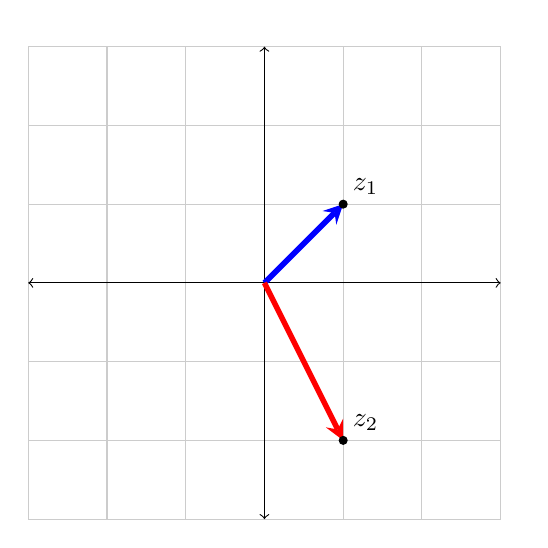
\begin{tikzpicture}
        \draw[thin,gray!40] (-3,-3) grid (3,3);
        \draw[<->] (-3,0)--(3,0) node[right]{$\RE$};
        \draw[<->] (0,-3)--(0,3) node[above]{$\IM$};
        \draw[line width=2pt,blue,-stealth](0,0)--(1,1) node[anchor=east] at (1,1){};
        \draw[line width=2pt,red,-stealth](0,0)--(1,-2) node[anchor=east] at (1,-2){};
        \foreach \Point/\PointLabel in {(1,1)/z_1, (1,-2)/z_2}
        \draw[fill=black] \Point circle (0.05) node[above right] {$\PointLabel$};
        \end{tikzpicture}
\]
Using this idea, let us see how we can plot a complex function in a different way.

\begin{ex}{Plotting a Complex Function}
	Let's consider a complex function $f\colon \C \to \C$ given by the function
	\[
		f(z) = iz= -\IM(z)+i\RE(z).
	\]
	Recall that multiplication by $i$ rotates a complex number by an angle of $\pi/2$ in the counterclockwise direction. Thinking this way will help us understand what this function is doing.  For some more concrete results, we should compute a few values for this function
	\begin{align*}
		f(0)&= 0 & f(1)&=i & f(i)&= -1\\
		f(-1)&= -i & f(1+i)&= -1+i & f(-1 -i) &= 1 - i.
	\end{align*}
	We can plot these values as vectors emanating from the input point $z$. That is, we can place the arrow given by the output $f(z)$ at the point $z$.  
	\[
	        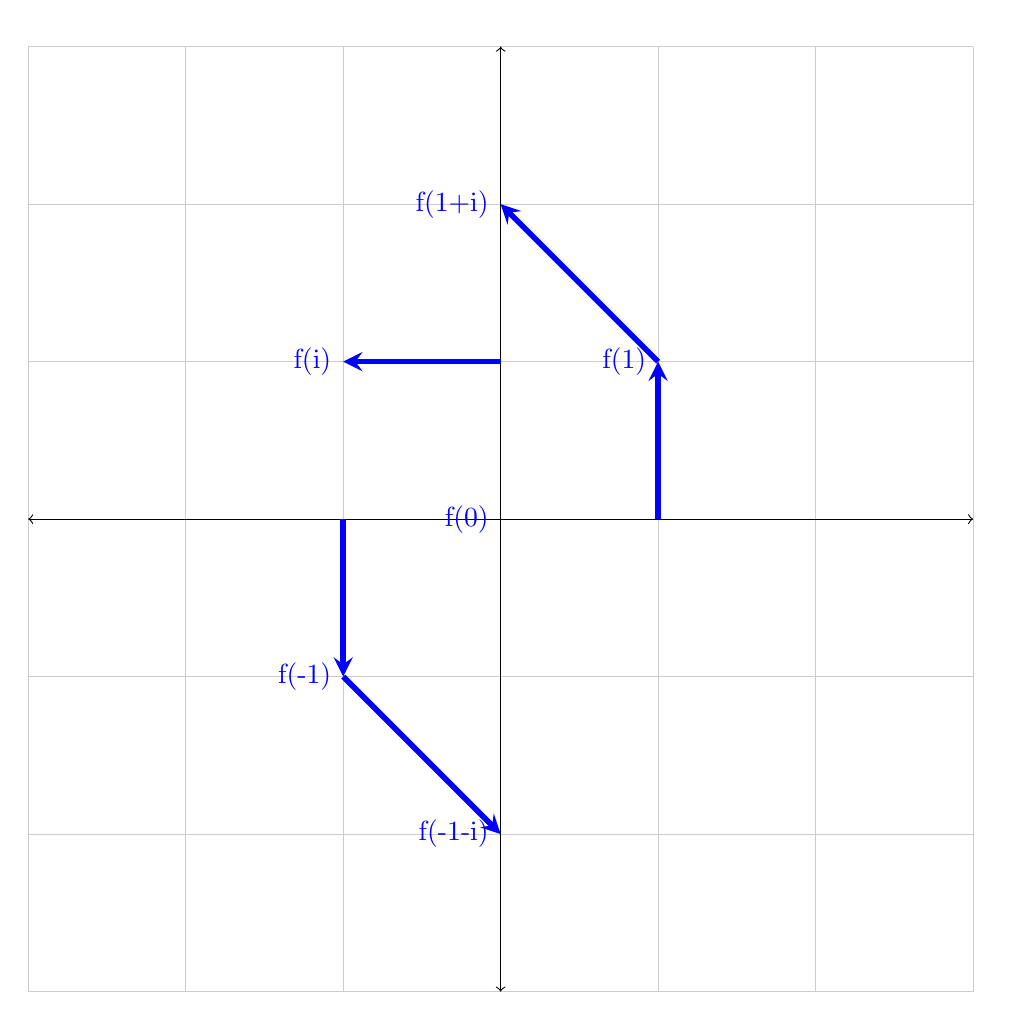
\begin{tikzpicture}[scale=2]
	        \draw[thin,gray!40] (-3,-3) grid (3,3);
	        \draw[<->] (-3,0)--(3,0) node[right]{$\RE$};
	        \draw[<->] (0,-3)--(0,3) node[above]{$\IM$};
	        \draw[line width=2pt,blue,-](0,0)--(0,0) node[anchor=east] at (0,0){f(0)};
	        \draw[line width=2pt,blue,-stealth](1,0)--(1,1) node[anchor=east] at (1,1){f(1)};
	        \draw[line width=2pt,blue,-stealth](-1,0)--(-1,-1) node[anchor=east] at (-1,-1){f(-1)};
	        \draw[line width=2pt,blue,-stealth](0,1)--(-1,1) node[anchor=east] at (-1,1){f(i)};
	        \draw[line width=2pt,blue,-stealth](1,1)--(0,2) node[anchor=east] at (0,2){f(1+i)};
	        \draw[line width=2pt,blue,-stealth](-1,-1)--(0,-2) node[anchor=east] at (0,-2){f(-1-i)};
	        \end{tikzpicture}
	  \]
	  We can then do this for many more input points to get a picture like the following.
		\begin{figure}[H]
			\centering
			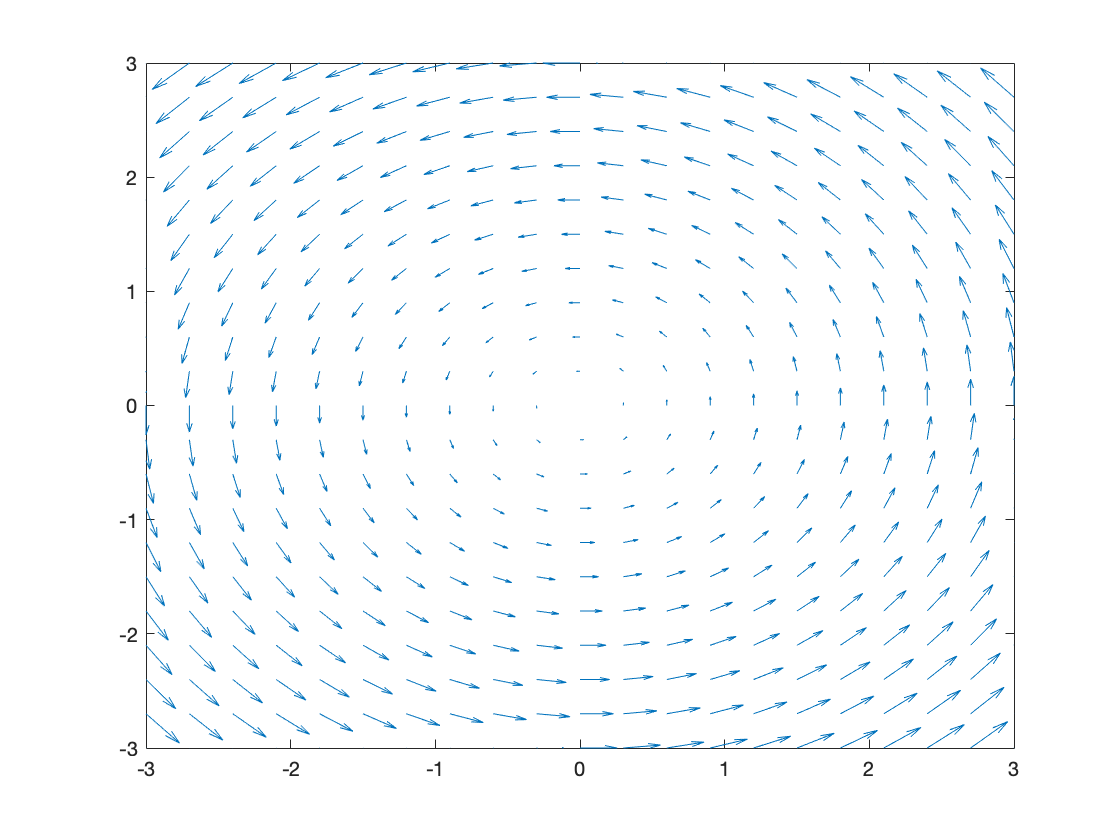
\includegraphics[width=\textwidth]{Figures_Part_5/complex_function_visual.png}
			\caption{A plot of various different outputs for their corresponding inputs.}
		\end{figure}
		What we see here is typically referred to as a vector field. We will get to this notion later on in the text.
\end{ex}
		
\subsection{Complex Valued Functions}

A major focus in this course is understanding the mathematics behind quantum mechanics.  For a chemist, this knowledge is rather important since modern theory is mostly quantum in nature.  What isn't quantum is likely thermodynamical or electrodynamical in nature and we will get to these topics a bit later on. 

Recall that wavefunctions are solutions to Schr\"odinger's equation.  In the broadest generality, wavefunctions are functions that are complex valued and whose domain of definition is on some region $\Omega$ in space $\R^3$.  More generally, we can allow for $\Omega$ to a be a region in other spaces as well. To restate this, we are considering a function of the form $\Psi\colon \Omega \to \C$ where we will specify what the domain $\Omega$ is. Previously, we looked at models in lower dimensions (e.g., the free particle in the 1-dimensional box) since we have yet to properly discuss multivariate functions.  

For now, consider a complex function $\Psi\colon [a,b] \to \C$ that has a single real variable as an input.  Thus, we define this function by $\Psi(x)=z$, where $z\in \C$.  Of course, we get the Cartesian decomposition
\[
\Psi(x)=u(x)+iv(x),
\]
or the polar decomposition
\[
\Psi(x)=r(x)e^{i\theta(x)}.
\]

The great thing in this case is that we can differentiate and integrate wavefunctions in a way that's no different than single variable real functions!  Fundamentally, this is due to the fact that our understanding of the derivative has only been defined for a single real value input. We will deepen our understanding later.  So, for a wavefunction we have that
\[
\Psi'(x)=u'(x)+iv'(x),
\]
and in the polar case we have
\[
\Psi'(x)=r'(x)e^{i\theta(x)}+r(x)e^{i\theta(x)}\theta'(x),
\]
which follows from the chain rule.

\begin{exercise}
	Verify the polar derivative above is correct.
\end{exercise}

Integration follows the fundamental theorem of calculus and hence we have
\[
\int_a^b \Psi'(x)dx = \Psi(b)-\Psi(a).
\]
So, for example, in the cartesian representation we have
\[
\int_a^b \Psi'(x)dx = \int_a^b u'(x)dx+i\int_a^b v'(x)dx = [u(b)-u(a)]+i[v(b)-v(a)].
\]

\begin{remark}
	Complex functions (i.e., functions with complex valued inputs) have different behavior with integration and differentiation which we will not discuss at all.  The closest we will get to this structure is calculus in $\R^2$.
\end{remark}

\begin{ex}{A Line in $\C$}{line_in_C}
	Let's consider the complex function $f\colon \R \to \C$ given by the Cartesian representation 
	\[
	f(x) = x+ix.
	\]
	How should we think of this function? For one, we can see how the output changes as the input changes by testing a few values
	\begin{align*}
		f(0)&=0 & f(1)&=1+i\\
		f(-1)&=-1-i & f(2)&=2+2i.
	\end{align*}
	We can also visualize this function in the following way. For every input, we will just place the complex output into the complex plane. Unlike plotting real functions, we will have to pay a bit more attention to what the input value is.
	\[
	    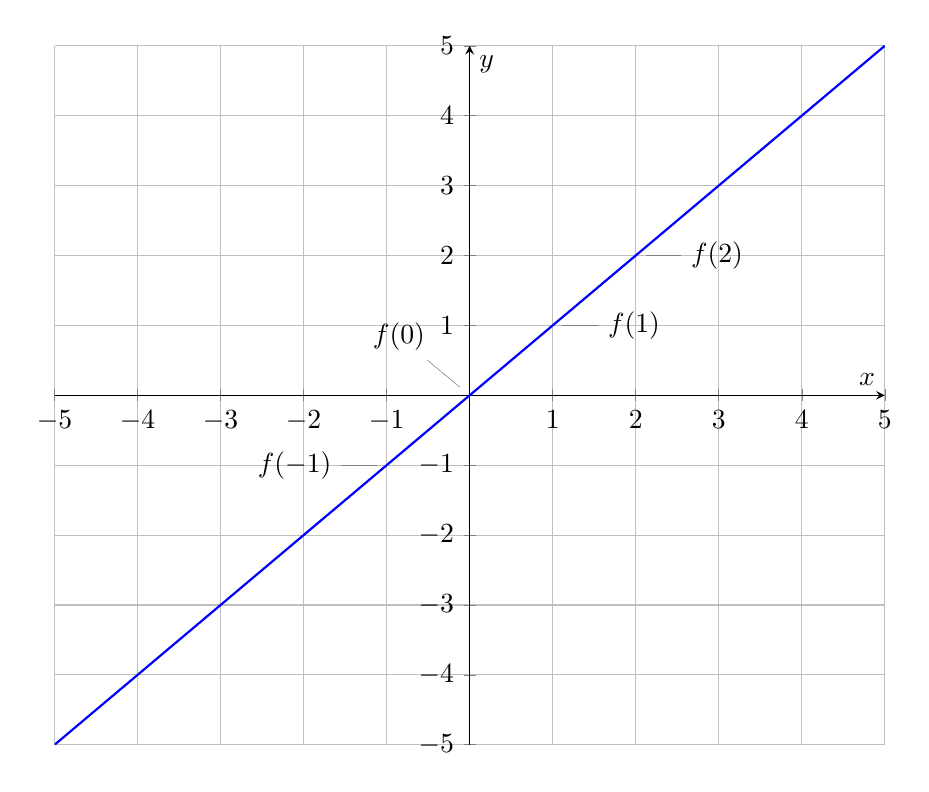
\begin{tikzpicture}[baseline]
	    \begin{axis}[
	    axis y line=center,
	    axis x line=middle,
	    %axis equal,
	    grid=both,
	    xmax=5,xmin=-5,
	    ymin=-5,ymax=5,
	    xlabel=$x$,ylabel=$y$,
	    xtick={-10,...,10},
	    ytick={-10,...,10},
	    width=\textwidth,
	    anchor=center,
	    ]
	    \addplot [mark=none, blue, thick]{x} ;
	    \addplot [mark=none] coordinates {(1,1)} node[pin=0:{$f(1)$}]{};
	    \addplot [mark=none] coordinates {(2,2)} node[pin=0:{$f(2)$}]{};
	    \addplot [mark=none] coordinates {(-1,-1)} node[pin=180:{$f(-1)$}]{};
	    \addplot [mark=none] coordinates {(0,0)} node[pin=135:{$f(0)$}]{};
	    \end{axis}
	    \end{tikzpicture}
	    \]
	   We often refer to this type of function as a curve or, in the complex case specifically, a contour.  Again, we will revisit curves later on in this text.
\end{ex}

\begin{ex}{Wavefunctions in the Box}{wavefunctions_in_1dbox}
	Let $\Omega=[0,L]$ and recall that the normalized states of the particle in the 1-dimensional box were given by
	\[
		\psi_n(x)=\sqrt{\frac{2}{L}} \sin\left(\frac{n \pi x}{L}\right).
	\]
	Recall as well that we could write a wavefunction as a superposition of states by
	\[
		\Psi(x)=\sum_{n=0}^\infty a_n \psi_n(x).
	\]
	Though these states are real valued, there is no physics that requires this.  Similarly, the coefficients $a_n$ are also not constrained to be real valued constants either.  In the broadest generality, $\Psi$ can be a complex valued function and the coefficients $a_n$ can be complex as well.

	Fundamentally, this is due to the physical understanding of the solutions to Schr\"odinger's equation. When we are looking for physically meaningful interpretations of a wavefunction, we must evaluate an integral. We can think of this act of integration as performing a measurement.  For example, let $[a,b]$ be a subinterval of $[0,L]$, then we can compute the probability of the particle with wavefunction $\Psi(x)$ to be in the region $[a,b]$ by 
	\[
		P_{[a,b]}(\Psi) = \int_a^b \|\Psi(x)\|^2dx,
	\]
	where we have the pointwise modulus of the complex valued function
	\[
		\|\Psi(x)\|^2 = \Psi^*(x)\Psi(x),
	\]
	where $~^*$ indicates the complex conjugate.  Say we take the cartesian representation for $\Psi(x)$ by $\Psi(x)=u(x)+iv(x)$, then
	\[
		\|\Psi(x)\|^2 = u^2(x)+v^2(x).
	\]
	
	Let $\Psi(x)=\frac{1}{\sqrt{2}}\psi_1(x)+\frac{1}{\sqrt{2}}\psi_2(x)$ be a superposition state.  We can compute the probability that the particle is in the first half of the region $[0,L]$ by computing
	\begin{align*}
		P_{[0,L/2]}(\Psi)&=\int_{0}^{L/2}  \|\Psi(x)\|^2 dx \\
			&=\int_{0}^{L/2} \frac{1}{2}\psi_1^2(x)+ \psi_1(x)\psi_2(x)+\frac{1}{2}\psi_2^2(x)dx\\
			&=\int_{0}^{L/2}\frac{1}{2} \left(\sqrt{\frac{2}{L}}\sin\left(\frac{\pi x}{L}\right)\right)^2 + \sqrt{\frac{2}{L}}\sin\left(\frac{\pi x}{L}\right)\sin\left(\frac{2\pi x}{L}\right)+ \frac{1}{2}\left(\sqrt{\frac{2}{L}}\sin\left(\frac{2\pi x}{L}\right)\right)^2dx\\
			&=\frac{1}{2}+\frac{4}{3\pi}\\
			&\approx .924.
	\end{align*}
	Through this calculation we have found that the probability that the particle is the first half of box is about $92.5\%$.  Since the particle must be in the box, it follows that the probability of the particle being in $[L/2,L]$ must be $1-\frac{1}{2}-\frac{4}{3\pi}$ or roughly $7.5\%$.  This is quite different than we would expect classically!

	We can plot the functions used above to see why this is the case.
	\begin{figure}[H]
	\centering
		\begin{subfigure}[h]{0.49\textwidth}
			\centering
			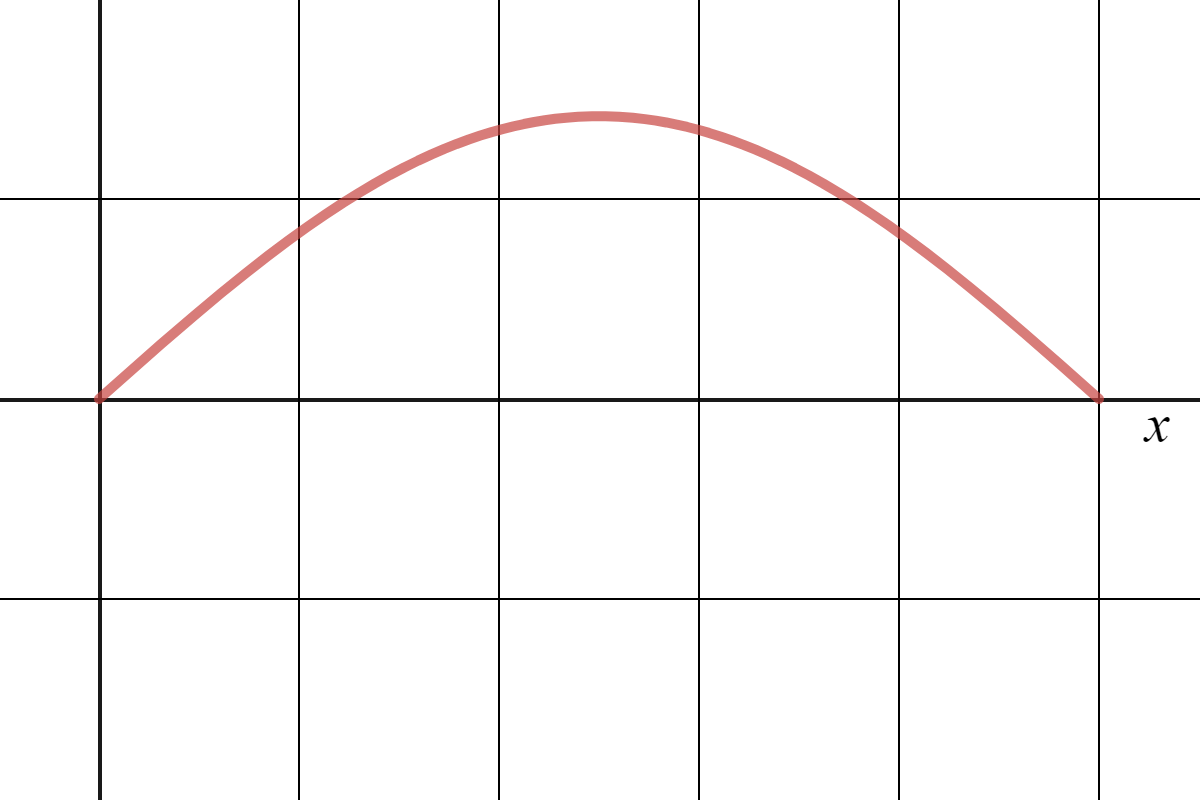
\includegraphics[width=.8\textwidth]{Figures_Part_5/psi_1.png}
			\caption{Normalized state $\psi_1(x)$.}
		\end{subfigure}
		~
		\begin{subfigure}[h]{0.49\textwidth}
			\centering
			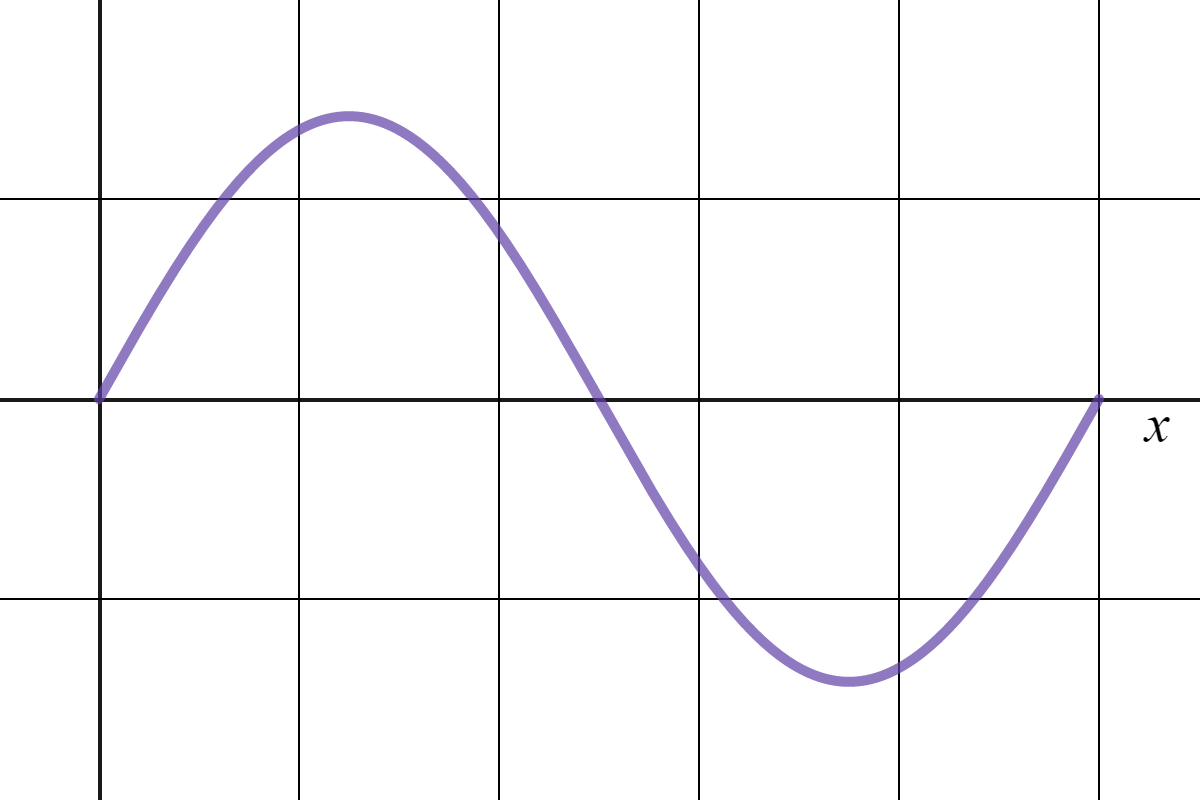
\includegraphics[width=.8\textwidth]{Figures_Part_5/psi_2.png}
			\caption{Normalized state $\psi_2(x)$.}
		\end{subfigure}
		\\
		\begin{subfigure}[h]{0.49\textwidth}
			\centering
			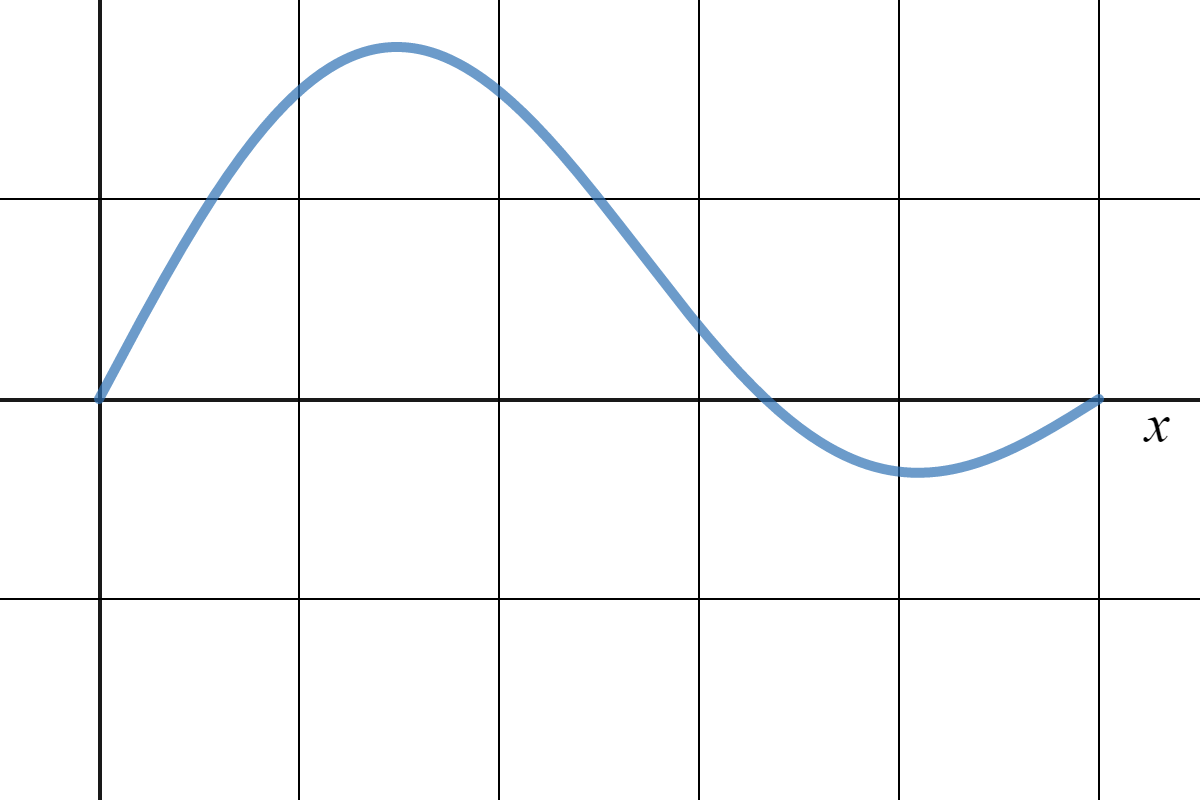
\includegraphics[width=.8\textwidth]{Figures_Part_5/Psi.png}
			\caption{The wavefunction $\Psi(x)$.}
		\end{subfigure}
		~
		\begin{subfigure}[h]{0.49\textwidth}
			\centering
			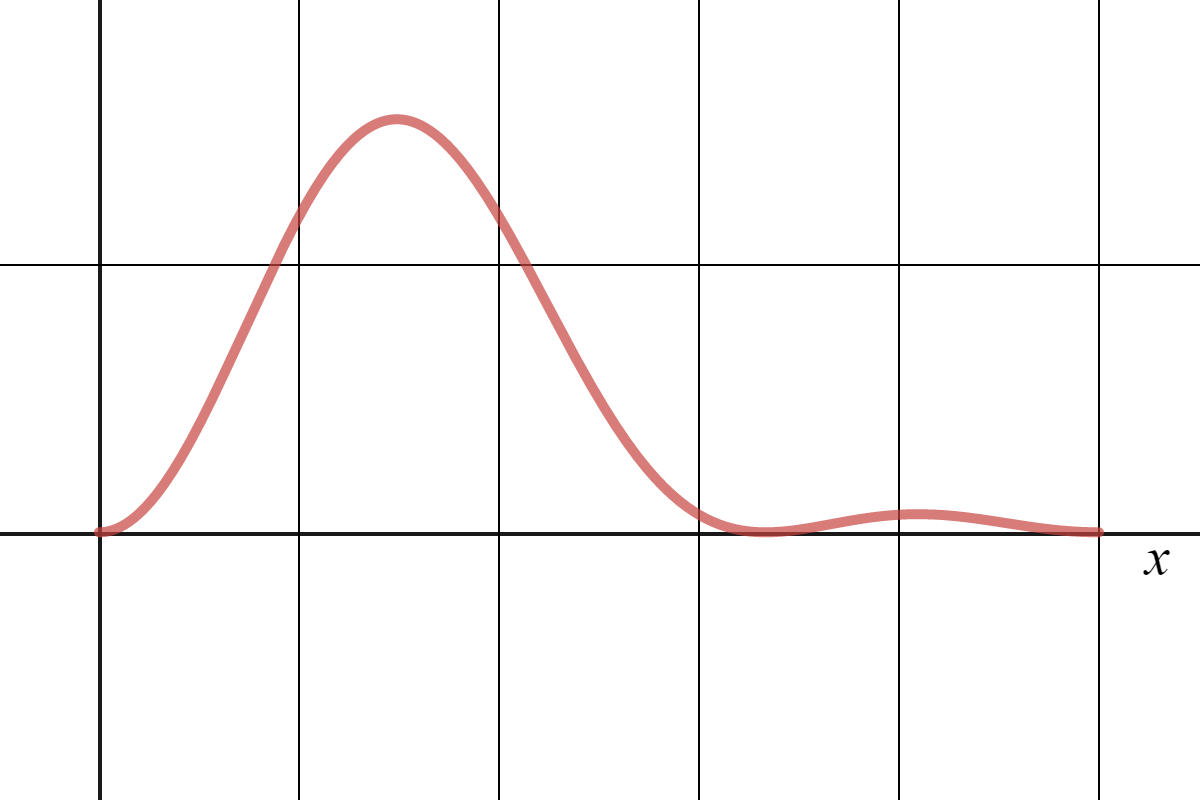
\includegraphics[width=.8\textwidth]{Figures_Part_5/prob_Psi.png}
			\caption{The probability function $\|\Psi(x)\|^2$.}
		\end{subfigure}
	\end{figure}
	The plots above of course show us that the integration makes sense.  We can see in (d) that the function that describes the probability is heavily weighted towards the first half of the interval $[0,L]$. One may then wonder if this is always true? That is, if I were to check back later in time, is the probability still distributed in the same way? The answer is no.  Later, we will introduce the time dependent version of the Schr\"odinger equation where we will see that these wavefunctions also evolve over time.  To some extent, we can see a bit of this behavior now.
	
	If we instead change our wavefunction by introducing a phase difference for each of the components.  What will happen in this case? If you have seen the double slit experiment, you may guess that introducing a phase difference can change the result (as phase difference causes interference). Instead of the $\Psi(x)$ above, take 
	\[
		\tilde{\Psi}(x) = \frac{e^{i\theta}}{\sqrt{2}} \psi_1(x) + \frac{e^{i\phi}}{\sqrt{2}} \psi_2(x).
	\]
	In this case, all we have done is made the wavefunction complex.  If, however, we consider the probability distribution given by this new wave function, we find
	\[
		\|\tilde{\Psi}(x)\|^2 = \tilde{\Psi}^*(x)\tilde{\Psi}(x) = \frac{1}{2}\psi_1^2(x)+\frac{e^{i(\theta-\phi)}}{2}\psi_1(x)\psi_2(x)+\frac{e^{i(\phi-\theta)}}{2}\psi_1(x)\psi_2(x)+\frac{1}{2}\psi_2^2(x).
	\]
	This is now slightly different! However, we can note that
	\[
		\frac{e^{i(\theta-\phi)}+e^{i(\phi-\theta)}}{2} = \cos(\theta-\phi),
	\]
	and hence we have
	\[
		\|\tilde{\Psi}(x)\|^2 = \tilde{\Psi}^*(x)\tilde{\Psi}(x) = \frac{1}{2}\psi_1^2(x)+\cos(\theta-\phi)\psi_1(x)\psi_2(x)+\frac{1}{2}\psi_2^2(x).
	\]
	So the phase difference $\delta=|\theta-\phi|$ between the two states causes the wavefunction to change. In the first example with $\Psi(x)$, the phase difference $\delta=0$ and we observed the probability function $\|\Psi(x)\|^2$.  However, let us see what happens as we change the phase.
	\begin{figure}[H]
	\centering
		\begin{subfigure}[h]{0.49\textwidth}
			\centering
			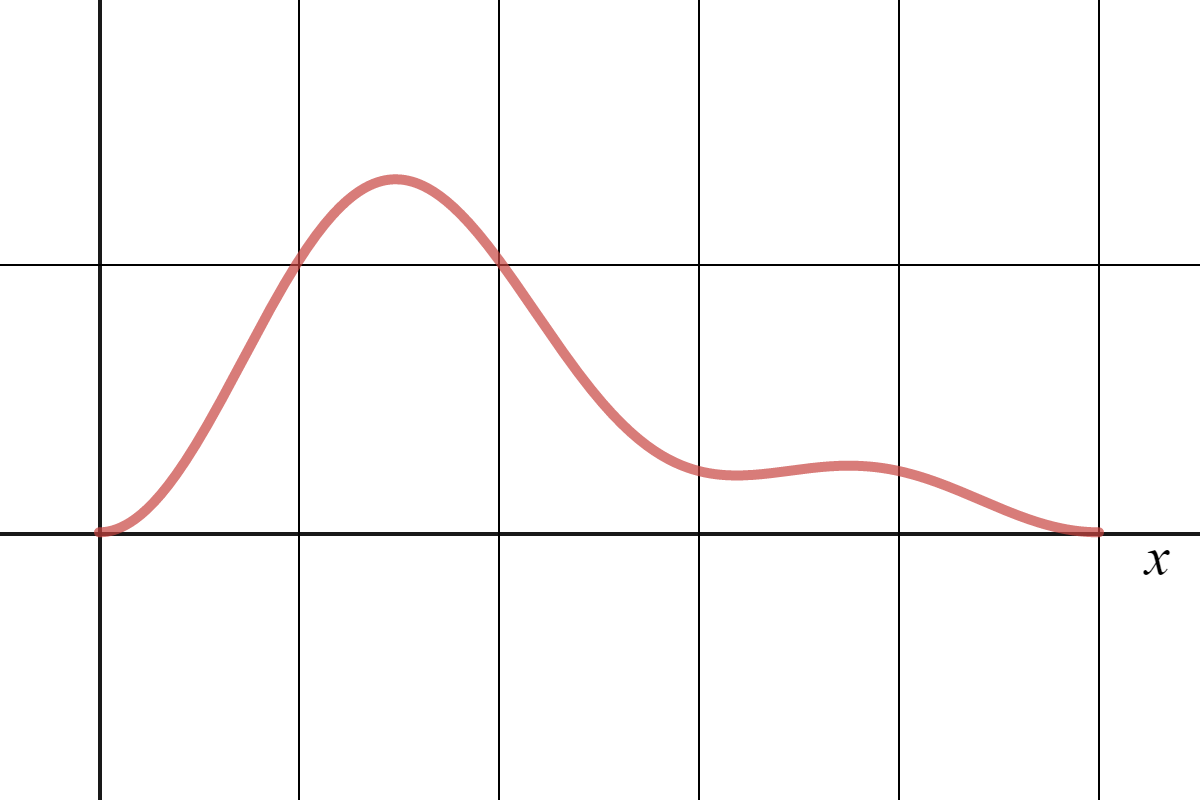
\includegraphics[width=.8\textwidth]{Figures_Part_5/prob_Psi_pi4.png}
			\caption{Phase difference $\delta=0$.}
		\end{subfigure}
		~
		\begin{subfigure}[h]{0.49\textwidth}
			\centering
			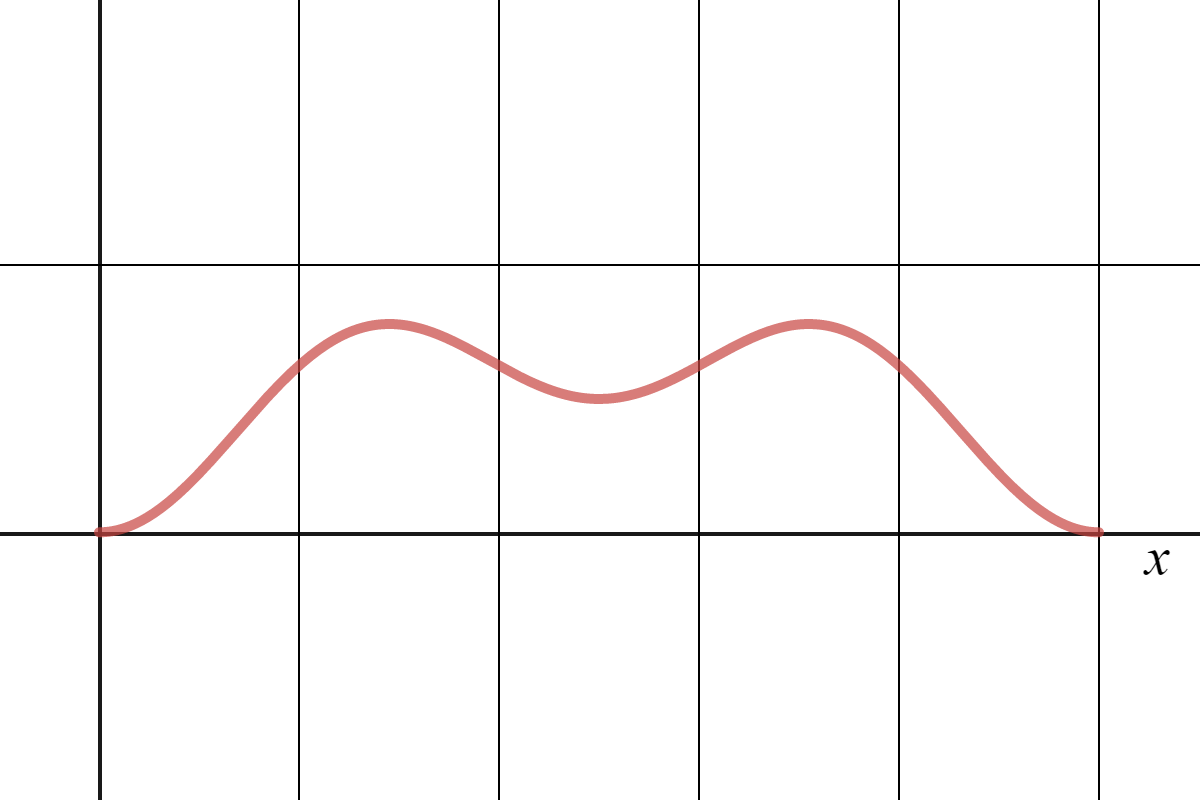
\includegraphics[width=.8\textwidth]{Figures_Part_5/prob_Psi_pi2.png}
			\caption{Phase difference $\delta=\frac{\pi}{3}$.}
		\end{subfigure}
		\\
		\begin{subfigure}[h]{0.49\textwidth}
			\centering
			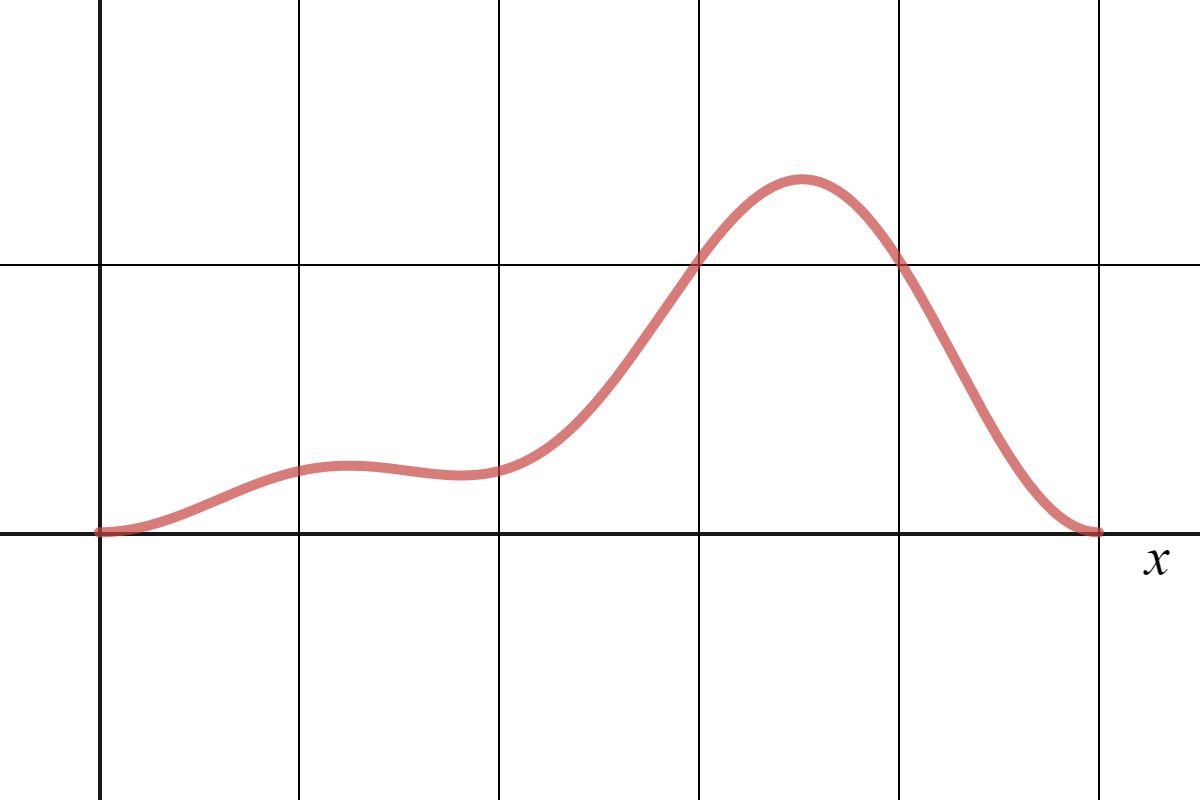
\includegraphics[width=.8\textwidth]{Figures_Part_5/prob_Psi_3pi4.png}
			\caption{Phase difference $\delta=\frac{2\pi}{3}$.}
		\end{subfigure}
		~
		\begin{subfigure}[h]{0.49\textwidth}
			\centering
			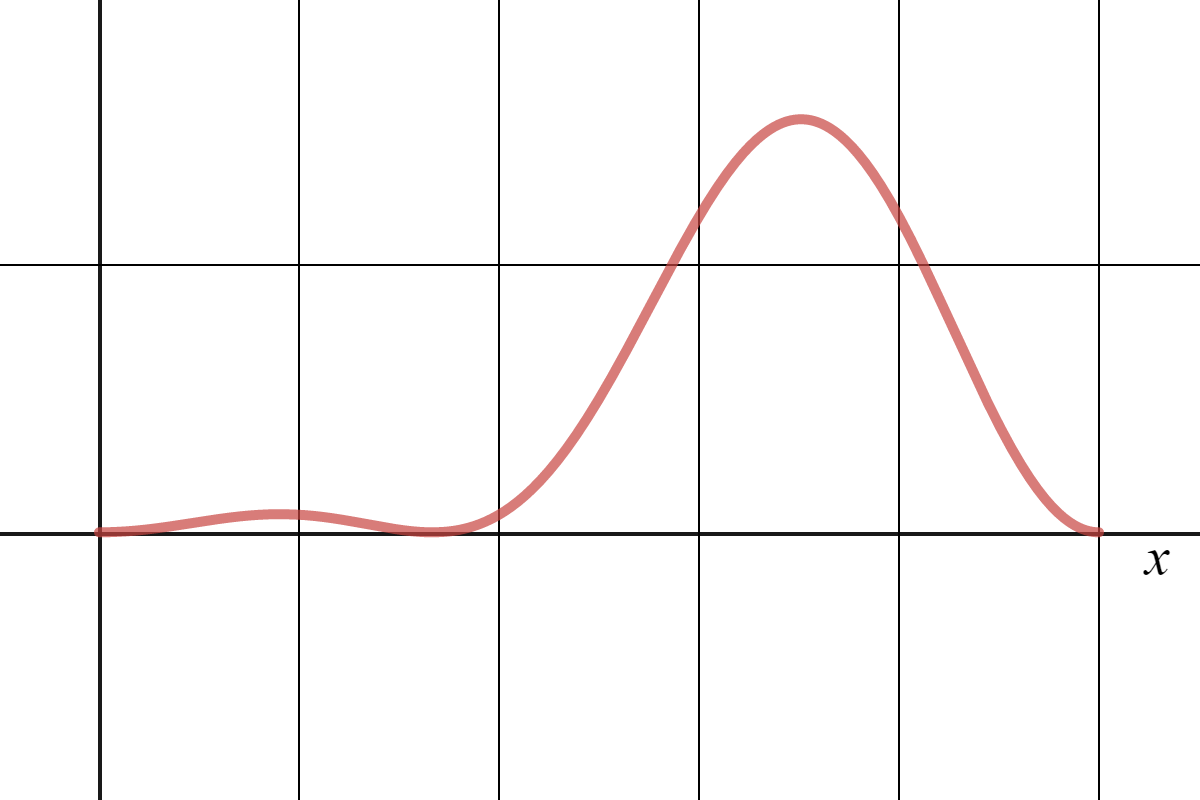
\includegraphics[width=.8\textwidth]{Figures_Part_5/prob_Psi_pi.png}
			\caption{Phase difference $\delta=\pi$.}
		\end{subfigure}
	\end{figure}
	 Interestingly enough, it seems that the phase difference ``moves" the particle around in the box. Of course, the particle itself is not moving, but the function that represents the likelihood of its position changes as the phase changes.  The largest difference in phase is $\pi$, and when we see this, we find that the distribution given by $\|\tilde{\Psi}(x)\|^2$ is the mirror image of the original $\|\Psi(x)\|^2$.  

	There are two important remarks to note here.
	\begin{enumerate}[1.]
		\item We can change the global phase of the system without changing the probability of measurement.  That is, $e^{i\theta}\Psi(x)$ has no discernable difference from $\Psi(x)$ (you can verify this from the work above).
		\item This difference in phase seems to drive some form of motion for a particle.  It is with this insight that we will later revisit the time dependent version of the Schr\"odinger equation and see how the time component relates to phase.
	\end{enumerate}
\end{ex}

\begin{remark}
	In a sense, the integral defined above $P_{[a,b]}(\Psi)$ is a real valued function with a function as an input.  Though we have not noted this until now, it becomes important in the future.
\end{remark}

All of this is to say that we must be able to work with complex valued functions.  They show up in physics and help us describe what we observe through nature.  It's important to remember that all measurements we make in a lab must be real valued, and so our mathematical models for these measurements must take that into account as well. 

\chapter{Hilbert Spaces}
\section{Introduction}
Recall the importance of the dot product in space.  Given two vectors $\vecu,\vecv \in \R^3$, we defined the dot product by
\[
\vecu \cdot \vecv = u_1v_1 + u_2v_2 + u_3v_3,
\]
and we also referred to this as an inner product.  The dot product allowed us to project a vector onto its components by, for example,
\[
\vecu \cdot \xhat = u_1.  
\]
This was extremely useful for us.  On top of that, the dot product provided us a means of computing the length of a vector by putting
\[
\|\vecu\|=\sqrt{\vecu\cdot\vecu}.
\]
Underlying much of the theory of space was this structure. 

Later, we introduced the Hermitian inner product on complex vectors.  As it turns out, this inner product is strictly more general than the dot product.  If we had two vectors $\veca,\vecb\in \C^n$ (i.e., vectors with $n$ complex number entries) then we defined the inner product by
\[
\langle \veca,\vecb \rangle = \sum_{j=1}^n a_jb_j^*.
\]
Note that if $\veca$ and $\vecb$ only have real entries, then the complex conjugate $b_j^*=b_j$ and we are left with the typical dot product for $\R^n$.  It suffices to say, that we need only care about this Hermitian inner product. In the same vein, we receive all the wonderful benefits of the dot product.  For example, we can project a vector by taking
\[
\xhat_1 = \begin{pmatrix} 1 \\ 0 \\ 0 \\\vdots \\ 0 \end{pmatrix}
\]
and computing
\[
\langle \veca,\vecx_1\rangle = a_1.
\]
Likewise, the length of a complex vector is given by
\[
\|\veca\|=\sqrt{\langle \veca,\veca\rangle}.
\]
Nothing is lost from this more general approach, and this more general approach extends far beyond finite dimensional complex vectors!

\subsection{Infinite Dimensions}

The dimension of a vector is the number of entries needed to fully describe the vector.  From the examples before, we can say that the vectors $\vecu,\vecv\in \R^3$ are 3-dimensional real vectors and the vectors $\veca,\vecb \in \C^n$ are $n$-dimensional complex vectors.  There is no restriction on the size of $n$, and $n$ can in fact be infinite!

This section of the text is primarily concerned with extending our linear algebra techniques to the infinite dimensional case.  Though this may sound ominous, it simply builds upon what we already know.  In essence, we will combine our knowledge of functions, infinite series, integrals, and linear algebra to complete the theory for infinite dimensions.  Put simply, functions will play the role of vectors while series and integrals will play the role of inner products.  This viewpoint places us viewing mathematics from the top, where we can always reduce the general story to something more specific when need be. Ultimately, this allows one to understand one general structure instead of many individual ones.

\section{Function Spaces}

\textcolor{red}{add here}

\section{Inner Products}

Before we define general inner products, let us recall the definition of a vector space.  In the prequel, we had that a vector space $V$ over some field $\field$ (the numbers we choose as entries) is a set containing vectors that satisfy eight different properties.

\begin{exercise}
	Find the definition in the previous text and review it.
\end{exercise}

\begin{df}{Inner Product}{inner_prod_general}
An \boldgreen{inner product} on a vector space $V$ over a field $\field$ is a bilinear (sometimes sesquilinear) function
\[
\innprod{\cdot}{\cdot} \colon V \times V \to \field,
\]
that satisfies
\begin{enumerate}[i.]
	\item (Nondegenerate) For a $\veca\in V$ we have that $\innprod{\veca}{\veca} =0$ if and only if $\veca=\zerovec$;
	\item (Positive definite) For any nonzero $\veca \in V$ we have that $\innprod{\veca}{\veca} > 0$;
	\item (Symmetric) For any $\veca,\vecb\in V$ we have that $\innprod{\veca}{\vecb} = \innprod{\vecb}{\veca}$. If the vector space is complex, then we have conjugate symmetry $\innprod{\veca}{\vecb}=\innprod{\vecb}{\veca}^*$.
\end{enumerate}
What we are denoting is a function $\innprod{\cdot}{\cdot}$ that has two vectors ($V\times V$) as inputs where see $\cdot$ and outputs some number in the designated field $\field$. When we say bilinear, we mean that the function is linear in each input. For example, we have for vectors $\veca,\vecb,\vecc\in V$ and a scalar $\alpha \in \field$ that
\[
\innprod{\alpha\veca + \vecb}{\vecc} = \alpha \innprod{\veca}{\vecc} + \innprod{\vecb}{\vecc},
\]
which shows the linearity in the first input.  The second input is linear as well.

Similarly, if the field $\field=\C$, then the inner product need be sesquilinear in that we instead have the addition of a complex conjugate in the second position. That is, let $\alpha,\beta\in \C$ and we have
\[
\innprod{\alpha\veca + \vecb}{\beta\vecc} = \alpha \beta^*\innprod{\veca}{\vecc} + \beta^*\innprod{\vecb}{\vecc}.
\]
The first position is simply linear.
\end{df}

\begin{exercise}
	Verify that the dot product for $\R^n$ and the Hermitian inner product for $\C^n$ are indeed inner products.
\end{exercise}

Since we have previously covered two different inner products for the finite dimensional vector spaces $\R^n$ and $\C^n$, we can use our intuition from these spaces with their inner product structure to define other important inner products.  We have in fact come across another example while studying the particle in the 1-dimensional box.  Recall that the problem we solved was the equation
\[
-\frac{\hbar^2}{2m} \frac{d^2 \Psi(x)}{dx^2} = E\Psi(x),
\]
on the region $[0,L]$, where $\Psi(x)$ is the wavefunction.  We also imposed the boundary conditions that $\Psi(0)=\Psi(L)=0$ since the particle cannot be found on the boundary of this domain.  

We found that the solutions to this equation were the normalized states 
\[
\psi_n(x) = \sqrt{\frac{2}{L}} \sin\left(\frac{n\pi x}{L}\right),
\]
with corresponding energies $E_n = \frac{n^2h^2}{8mL^2}$. Then, a wavefunction could be written as a linear combination of these states by
\[
\Psi(x) = \sum_{n=1}^\infty a_n \psi_n(x),
\]
where $a_n \in \C$.  In order for the wavefunction $\Psi(x)$ to be normalized, we required that
\[
\sum_{n=1}^\infty \|a_n\|^2=1.
\]
Now, we can consider a set $V$ of all the possible wavefunctions for the above problem as well as the zero function (which is indeed a solution to the problem, but it is not physically meaningful).

\begin{exercise}
	Show that $V$ is a vector space. 
\end{exercise}

We can add an inner product to the vector space $V$ by defining the inner product on two wavefunctions $\Psi$ and $\Phi$ by
\[
\innprod{\Psi}{\Phi} \coloneqq \int_0^L \Psi(x) \Phi^*(x)dx.
\]
To see that this is an inner product, we need to show that the above function is sesquilinear and satisfies the three conditions for an inner product (nondegeneracy, positive definite, and symmetric).  Sesquilinearity follows from the linearity of the integral in that we have
\begin{align*}
	\innprod{\Psi}{\Phi+\alpha \Theta} &= \int_0^L \Psi(x)(\Phi(x)+\alpha \Theta(x))^*dx \\
	&= \int_0^L \Psi(x) \Phi(x)\Phi^*(x)dx+\alpha^* \int_0^L \Psi(x) \Theta^*(x)dx\\
	&= \innprod{\Psi}{\Phi}+\alpha^* \innprod{\Psi}{\Theta}.
\end{align*}
Showing the linearity in the first argument is analogous but there will not be a complex conjugate.  

Next, we can see that the inner product is nondegenerate by noting that if we take the zero function 0, we have
\[
\innprod{0}{0} = \int_0^L 0 dx = 0,
\]
and if we have that
\[
0=\innprod{\Psi}{\Psi}  = \int_0^L \Psi(x)\Psi^*(x)dx = \int_0^L \|\Psi(x)\|^2dx,
\]
it must be that $\|\Psi(x)\|=0$ since this integral cannot be zero otherwise.  Hence, $\Psi(x)$ is the zero function and we have that the inner product is indeed nondegenerate.

By the above work, if $\Psi(x)$ is not the zero function, then $\|\Psi(x)\|^2>0$ and thus we have
\[
\innprod{\Psi}{\Psi}>0.
\]
Hence, the inner product is positive definite.

Lastly, we can see that the inner product is symmetric by taking the Cartesian representation for $\Psi(x)$ by $\Psi(x)=a(x)+ib(x)$ and for $\Phi(x)=c(x)+id(x)$ and noting
\begin{align*}
	\Psi(x)\Phi^*(x) &= (a(x)+ib(x))(c(x)-id(x))\\
		&= (a(x)c(x)+b(x)d(x))+i(b(x)c(x)-a(x)d(x)),
\end{align*}
and
\begin{align*}
	\Phi(x)\Psi^*(x) &= (c(x)+id(x))(a(x)-ib(x))\\
		&= (a(x)c(x)+b(x)d(x))+i(a(x)d(x)-b(x)c(x),
\end{align*}
which means that we have
\[
\innprod{\Psi}{\Phi}=\innprod{\Phi}{\Psi}^*.
\]
Thus we have shown that this is indeed an inner product.

\section{Inner Product Spaces}

Given a vector space $V$ with an inner product, we refer to the vector space as an \boldgreen{inner product space}.  In fact, all the vector spaces we have dealt with are inner product spaces! We tend to prefer working with these spaces as they allow us to nicely compare vectors (like we can with the dot product) and we can also compute lengths and distances.  Needless to say, inner product spaces are immensely important in the physical world.

However, when the vector space is not finite dimensional (such as the space of solutions to the 1-dimensional box with the added zero function), we must be a bit more careful.  Without going into far too much detail, we must add one other attribute to these spaces to make them work as we need.  In this case, we must require that the inner product space is also \boldgreen{complete}.  A space is complete if and only if all Cauchy sequences in the space converge. We call a complete inner product space a \boldgreen{Hilbert space}.

\begin{exercise}
	We defined a Cauchy sequence in the prequel. Find the definition.
\end{exercise}

This extra requirement rules out some oddities and makes the infinite dimensional space much more like the finite dimensional spaces such as $\R^n$ and $\C^n$.  We showed in the prequel that in $\R$ a convergent sequence is also Cauchy. That is, the definitions are analogous. The same happens to be true in $\R^n$ and $\C^n$ (you can picture taking a sequence of vectors instead of a sequence of real numbers).  Thus, in a Hilbert space, Cauchy and convergent are again equal. Let us see why one should believe this.

\begin{ex}{A Cauchy Sequence of Functions}{cauchy_functions}
	Before, we studied power series that define functions.  We would write
	\[
		f(x) = \sum_{n=0}^\infty a_n x^n,
	\]
	where $x$ is in the domain of convergence for the series.  As we worked through what it meant for a series to converge, we found that we could view a series as a sequence of partial sums.  That is, for each value of $x$ we can create a sequence $\{A_n(x)\}_{n=0}^\infty$ by letting
	\[
		A_N(x) = \sum_{n=0}^N a_n x^n.
	\]
	We noted that as we increased $N$, the function $A_N(x)$ became closer and closer to the function $f(x)$.  This was entirely reasonable as if the contrary were true, at some point a large $N$ would provide us a worse approximation to $f(x)$.  

	The completeness assumption for a Hilbert space will give us this ability.  It will allow one to properly approximate quantities such as infinite sums of functions in a way that makes intuitive sense.  
\end{ex}

No more detail is needed on the notion of completeness. We will completely avoid spaces that are not complete as they behave badly.  Take the completeness of any space as given unless it is mentioned otherwise. 

\section{Symmetries}

As previously discussed, symmetry is an important aspect of problem solving that is present in most physical systems.  The prior example is no exception.  We discussed the phase of a complex function and viewed this in an example from quantum mechanics.  There, we found that when a wavefunction is altered by adding a global phase, the probability of making a measurement is not changed.  This is in fact a specific example of something far more general.  But in this case for the particle in the 1-dimensional box, we can see that if alter two wave functions by the same phase and take the inner product
\begin{align*}
\innprod{e^{i\theta} \Psi}{e^{i\theta}\Phi} &= \int_0^L e^{i\theta} \Psi(x) (e^{i\theta}\Phi(x))^*dx \\
	&= \int_0^L e^{i\theta}\Psi(x)e^{-i\theta}\Phi^*(x)dx\\
	&= \int_0^L \Psi(x)\Phi^*(x)dx\\
	&= \innprod{\Psi}{\Phi},
\end{align*}
then the inner product is not changed.  This is an example of a \boldgreen{unitary operator}. A unitary operator preserves the inner product between two vectors. That is, if we have vectors $\Psi$ and $\Phi$ from an Hilbert product space $H$, then $U$ is a unitary operator if $U\colon H \to H$ is onto and
\[
\innprod{U\Psi}{U \Phi} = \innprod{\Psi}{\Phi}.
\]

This is of course not special for just the particle in the 1-dimensional box either. Take the space $\R^2$ with two vectors $\vecu$ and $\vecv$. Then consider a matrix $[A]$ that is in the group $\Orth(2)$ (which means that $[A]$ is a matrix that solely rotates and or reflects vectors).
\begin{exercise}
	Recall the definition of the matrix group $\Orth(2)$.
\end{exercise}
Now, we can actually realize any matrix in $\Orth(2)$ as a reflection matrix, or a product of two reflection matrices. For the sake of example, take a reflection matrix
\[
\REF_\theta = \begin{pmatrix} \cos (2\theta) & \sin(2\theta) \\ \sin(2\theta) & -\cos(2\theta) \end{pmatrix},
\]
which reflects a vector about the line passing through the origin with angle $\theta$ measured from the $x$-axis.  Then letting
\[
\vecu = \begin{pmatrix} u_1 \\ u_2 \end{pmatrix} \qquad \textrm{and} \qquad \vecv = \begin{pmatrix} v_1 \\ v_2 \end{pmatrix},
\]
 we have
\[
\REF_\theta \vecu = \begin{pmatrix} \cos(2\theta)u_1+\sin(2\theta)u_2 \\  \sin(2\theta)u_1-\cos(2\theta)u_2 \end{pmatrix} \qquad \textrm{and} \qquad \REF_\theta \vecv = \begin{pmatrix} \cos(2\theta)v_1+\sin(2\theta)v_2 \\  \sin(2\theta)v_1-\cos(2\theta)v_2 \end{pmatrix}.
\]
\textcolor{red}{Put a picture here}
Then we can compute the inner product of the reflected vectors 
\begin{align*}
\innprod{\REF_\theta \vecu}{\REF_\theta \vecv}&= (\cos(2\theta)u_1+\sin(2\theta)u_2)(\cos(2\theta)v_1+\sin(2\theta)v_2 )\\
&\qquad + (\sin(2\theta)u_1-\cos(2\theta)u_2)(\sin(2\theta)v_1-\cos(2\theta)v_2)\\
&~\vdots\\
&= u_1v_1 + u_2v_2.
\end{align*}
\begin{exercise}
	Show the remaining steps in the above computation.
\end{exercise}
Since this is true for any reflection matrix, it will be true for any product of reflection matrices and hence the group of $\Orth(2)$ matrices are unitary transformations on the inner product space $\R^2$ (where the inner product is the standard dot product).

Every Hilbert space will have a group of unitary symmetries that preserve the inner product. Hence, we tend to have different names for these groups to reflect what the underlying Hilbert product space is. In the particle in a box case, the underlying symmetry is the (slightly inaptly named) unitary group $U(1)$ whereas the case for $\R^2$ it is the orthogonal group $\Orth(2)$.

\section{Bases}

In the case of finite dimensions, we found that we could construct a minimal set of vectors in a space $V$ such that any vector in $V$ can be written as a linear combination of those vectors.  We called such a set a basis.  Take for example, the space $\R^3$, where we had the standard orthonormal basis given by $\xhat$, $\yhat$, and $\zhat$.  We put
\[
\xhat = \begin{pmatrix} 1 \\ 0 \\ 0 \end{pmatrix}, \qquad \yhat = \begin{pmatrix} 0 \\ 1 \\ 0 \end{pmatrix}, \qquad \zhat = \begin{pmatrix} 0 \\ 0 \\ 1 \end{pmatrix},
\]
so that any vector
\[
\vecv = \begin{pmatrix} v_1 \\ v_2 \\ v_3 \end{pmatrix}
\]
could be written as
\[
\vecv = v_1 \xhat + v_2 \yhat + v_3 \zhat.
\]
The latter notation proves to be convenient in the infinite dimensional case.

We have already discovered one way in which we can form a basis for certain infinite dimensional spaces. This came in the form of power series. The major difference is that we have infinite sums to build functions instead of just finite sums to build vectors that live in spaces like $\R^n$ and $\C^n$. 

Let us continue on with the power series example.  For the sake of simplicity, we can consider the space of analytic functions on the region $[0,L]$ (recall that analytic meant the function has a power series).  Then, by definition, every function $f(x)$ in this space can be written as an infinite sum
\[
f(x)=\sum_{n=0}^\infty a_n x^n,
\]
so long as for every $x\in [0,L]$ we have that the above series converges. Thus we have really investigated infinite dimensional spaces and their bases a bit.  In this case, our basis is the set of all powers of $x$. That is to say, we use $\{x^0,x^1,x^2,x^3,\dots\}$ as our basis vectors and the coefficients are the $a_n$.  

In general, the definition of a basis that we have is already correct so long as we understand what it means in general to take a sum. In the previous example with power series, a sum could potentially be infinite.  In some cases (e.g., the Fourier transform) we will see that we may need to take an integral to be our method of summation.  

\subsection{Orthonormal Bases}

Once again, the finite dimensional case led us to discovering the usefulness of an inner product as a method for determining bases that are more useful.  Above, we mentioned the standard orthonormal basis for $\R^3$ which gives us the most natural decomposition of a vector.  Each of the vectors in this basis is of length one and is mutually orthogonal to one another.  Intuitively, this lets you describe a point in space by how much you must walk back or forth, left or right, and up or down to reach your desired location. The orthonormal basis gave us a way to naturally decompose a vector into separate components through the dot product. That is, we could find the $x$, $y$, or $z$-component of a vector and none of these components depend on the others. If you were to take a basis
\[
\vecu = \begin{pmatrix} 1 \\ 1 \\ 0 \end{pmatrix}, \qquad \vecv = \begin{pmatrix} 0 \\ 1 \\ 1 \end{pmatrix}, \qquad \vecw = \begin{pmatrix} 1 \\ 0 \\ 1 \end{pmatrix},
\]
then if you were to break a vector up into these components, you would find that there is some overlap between what each component describes.

\begin{exercise}
	Show the vectors $\vecu$, $\vecv$, and $\vecw$ above form a basis.  Then, to see that there is some overlap, you can find the components of a vector (of your choice) in the directions $\uhat$, $\vhat$, and $\what$. \emph{Hint: to see the overlap, determine the length of the vector you chose, and compare it to the length computed from components un the $\uhat$,$\vhat$, and $\what$.}
\end{exercise}

When a basis is not orthogonal, then to find independent components of a vector, you must somehow subtract off the overlap. This process is a bit tedious, so instead of giving an example, we can just assert the fact that orthogonal bases are indeed helpful. 

\begin{remark}
	Orthogonal bases in finite dimensions also appear when we find eigenvalues and eigenvectors for Hermitian matrices. Specifically, the set of eigenvectors corresponding to different eigenvalues for a Hermitian matrix are always orthogonal!
\end{remark}

One may wish that the Hilbert spaces would have some sense of a natural decomposition into different orthogonal components.  It turns out that in the realm of spaces we care about we can do this, and that some Hilbert spaces have particularly nice bases to work with. In the prequel, we studied series solutions to differential equations as a means of solving a large class of equations. During that time, we solved Legendre's equation and found the solutions were particularly nice.

Recall the equation we wished to solve was
\[
(1-x^2)f''(x)-2xf'(x)+m(m+1)f(x)=0
\]
with our domain $\Omega=[-1,1]$ and $m$ a non-negative integer ($m=0,1,2,\dots$). Ignoring the details, we found that there were solutions for each $m$ (which in some sense are like the eigenvalues for the 1-dimensional box).  The normalized solutions were known as the Legendre polynomials and the first few were
\begin{align*}
	f_0(x)&=\sqrt{\frac{1}{2}} & f_1(x)&=\sqrt{\frac{3}{2}} x\\
	f_2(x)&= \sqrt{\frac{5}{8}} (1-3x^2) & f_3(x)&=\sqrt{\frac{63}{8}}\left(x-\frac{5x^3}{3}\right).
\end{align*}
One may be wondering what we mean by normalized here. The solutions to the Legendre equation live in a Hilbert space whose inner product is given by
\[
\innprod{\Psi}{\Phi} = \int_{-1}^1 \Psi(x)\Phi(x)dx,
\]
in which these functions are normalized. That is, we have  
\[
\|f_i\|= \sqrt{\innprod{f_i}{f_i}} = 1,
\]
for every $i$. Note we do not need a complex conjugate in this inner product since these functions are all real valued. Moreover, it turns out that this set of polynomials is orthonormal since we also have
\[
\innprod{f_i}{f_j} = 0
\]
if $i\neq j$. Finally, the Legendre polynomials form a basis for the solution to the Legendre equation.  Specifically, we can write any other solution as a series of Legendre polynomials by
\[
f(x)= \sum_{n=1}^\infty a_n f_n(x),
\]
so long as the series converges for all values of $x$ in the domain $\Omega$.  

In the realm of quantum mechanics, the orthonormal basis of eigenfunctions are extremely important. Previously, we even donated these functions with the term \boldgreen{states}.  Though we never defined this term in the prequel, we now have a rough working definition.  When observing a quantum system, it is only possible to observe a particle in an eigenstate of the operator that is mathematical representation for the observation you are wishing to make.  We will define operators, eigenfunctions, and observables later.

\subsection{Expansion and Projection}



%\chapter{Linear Operators}
%\section{Matrices}
In the spirit of making analogies with the finite dimensional case, we will briefly revisit the idea of a linear transformations and matrices.  We previously studied linear transformations from one vector space to another. Most often we considered transformations of the form
\[
T \colon \R^3 \to \R^3
\]
which transformed space. We wrote
\[
T(\vecv)=\vecw.
\]
Recall that a linear transformation is one that satisfies
\[
T(\vecu+\alpha \vecv) = T(\vecu)+\alpha T(\vecv)
\]
for any two vectors $\vecu,\vecv \in \R^3$ and scalar $\alpha \in \R$. Since this transformation is linear, we found that we could represent this transformation as a matrix $[A]$ of nine numbers and multiply the vector by this matrix. So we wrote
\[
[A]\vecv = \vecw.
\]

Part of the reason we introduced the notion of linear transformations and not just matrices is that we will now need to ditch the notion of a matrix (unless you wish to write an infinite matrix, which, in some cases, you can do). Linear transformations are far more general and we can study their structure in a similar way that we did with matrices. 

\subsubsection{Linear Equations}
Matrices give rise to linear equations.  For example, we may be given a vector $\vecb \in \R^3$ and a $3\times 3$-matrix $[A]$ and will be asked to solve the equation
\begin{equation}
\label{eq:linear_eq}
[A]\vecx = \vecb,
\end{equation}
for the vector $\vecx$. This problem was solved by row reduction.  However, we also found that we could (in general) invert the matrix $[A]$ to produce $[A]^{-1}$.  This method was far more powerful since we could quickly solve the \ref{eq:linear_eq} with any given vector. Specifically, we have that
\[
\vecx = [A]^{-1}\vecb.
\]
In fact, the eigenvalue problem is extremely related to this idea as well.   Given the problem in \ref{eq:linear_eq}, we can isolate the matrix $[A]$ and decompose the action of the matrix into scaling on individual vectors. That is, we solve the eigen-equation
\[
[A]\evec = \lambda \evec.
\]
Scaling is an easy process to invert since we have
\[
[A]^{-1}\evec = \frac{1}{\lambda} \evec.
\]

\begin{exercise}
	Can you prove the above statement?
\end{exercise}

The moral is, if we can find a full set of eigenvalues and eigenvectors, then we can diagonalize our matrix by
\[
[\Lambda]=[P]^{-1}[A][P].
\]
The diagonal matrix $[\Lambda]$ is very easy to invert and so we can find
\[
[A]^{-1} = [P]^{-1}[\Lambda]^{-1}[P].
\]
This may seem like a bit more work than just inverting the matrix $[A]$, but this method allows us to see how the method is really working.  To some extent, you are performing this process when you compute $[A]^{-1}$ without directly mentioning so.

\begin{exercise}
	Can you show the work between the above steps?
\end{exercise}

We will return to this idea of inversion as we investigate more general operators.  


\subsubsection{Adjoints}

When we were given a matrix $[A]$ (whether real or complex) we could compute its adjoint by 
\[
[A]^\dagger=\left([A]^T\right)^*.
\]
That is, we can take the complex conjugate transpose of the matrix $[A]$. If $[A]$ is purely real, then this amounts to just taking the transpose. The notion of the adjoint was an important one in studying the eigenvalue problem.  For example, we stated that if a matrix is Hermitian (or self adjoint) then
\[
[A]^\dagger = [A].
\]
In this case, we know that all the eigenvalues of $[A]$ are real, and that the eigenvectors corresponding to different eigenvectors are orthogonal.  Recall, the eigenvalue problem
\[
[A]\evec = \lambda \evec.
\]
What the above says is that if $[A]$ is Hermitian, then $\lambda$ must be real.  In other words, one may say that the \boldgreen{spectrum} of a Hermitian matrix is always real.  The notion of a spectrum is of core importance in the study of quantum mechanics. Physicist Paul Dirac had developed a theory of quantum mechanics after Werner Heisenberg and Erwin Schr\"odinger where one computes the spectrum of the hamiltonian operator to find solutions.

\section{Linear Operators}

Just as we generalized the notion of vectors from the finite dimensional spaces into the infinite dimensional case, we will repeat with linear transformations.  The definitions of a vector space and linear transformation were properly general enough, but we will provide a new name for the linear transformations. Let $H$ be a Hilbert space. Then we have that a \boldgreen{linear operator} is a linear transformation $\linop \colon \hilbert \to \hilbert$.  Some may relax this definition a bit to allow for the input and output spaces to be different but we should not be concerned by this in any way. 

What is an example of a linear operator? Let us first choose a Hilbert space. We can, for example, choose the Hilbert space $\hilbert$ of analytic functions on a region $[0,L]$. Then consider the linear operator $x\colon \hilbert \to \hilbert$ which multiplies a given function by the variable $x$. Is this indeed linear?  Let us check by taking two function $f,g\in \hilbert$ and a constant $\alpha \in \R$ and note
\[
x(f(x)+\alpha g(x)) = xf(x)+\alpha xg(x),
\]  
which is indeed linear.  One should also check that, for example, $xf(x)$ is still an analytic function on $[0,L]$. Note that
\[
f(x) = \sum_{n=0}^\infty a_n x^n
\]
which converges on $[0,L]$. Then 
\[
xf(x) = \sum_{n=0}^\infty a_n x^{n+1}
\]
also converges on $[0,L]$.

\begin{exercise}
	Can you argue why this must be true? \emph{Hint: use the ratio test.}
\end{exercise}

Another example of a linear operator is taking the differential of a function. That is, the derivative $\linop=\frac{d}{dx}$ is an operator $\frac{d}{dx} \colon \hilbert \to \hilbert$.  Keeping $\hilbert$ as the analytic functions on $[0,L]$ then we can see that the derivative is linear by
\[
	\frac{d}{dx} (f(x)+\alpha g(x)) = \frac{df}{dx} +\alpha \frac{dg}{dx}.
\]
Previously one refers to these rules of the derivative as the sum rule and constant multiple rule. However, we should now just refer to this quality as the \boldgreen{linearity} of the derivative operator.  

These operators show up in the study of (ordinary) differential equations as we have seen before. Take for example the Hamiltonian operator
\[
\hat{H} = \frac{-\hbar^2}{2m} \frac{d^2}{dx^2} + V(x).
\]
This is a linear operator as well.  In fact, this operator $\hat{H}$ is even Hermitian which means its spectrum is real valued! This is a key component of the quantum theory as we only have the ability to measure real numbers.  We in fact require all observable operators to be Hermitian.  More on this in a bit.

\subsection{Adjoints}

Though we had defined adjoints of matrices through an operation, we need to instead provide a more general definition.  Let $\hilbert$ be a Hilbert space and $\linop$ a linear operator.  Then we define the \boldgreen{adjoint} $\linop^\dagger$ to be the unique operator satisfying
\[
\innprod{\linop\Psi}{\Phi} = \innprod{\Psi}{\linop^\dagger \Phi}.
\]
Let us see why this makes sense for the matrix case with an explicit example.

\begin{ex}{Matrix Adjoint}{matrix_adjoint}
	Let 
	\[
		[A] = \begin{pmatrix} 1 & 0\\ 1 & 1 \end{pmatrix}, \qquad \vecu = \begin{pmatrix} u_1 \\ u_2  \end{pmatrix}, \qquad \vecv = \begin{pmatrix} v_1 \\ v_2 \end{pmatrix}.
	\]
	Then let us take the inner (dot) product
	\[
	\innprod{[A]\vecu}{\vecv}.
	\]
	First, we compute
	\[
	[A]\vecu = \begin{pmatrix} u_1 \\ u_1+u_2 \end{pmatrix},
	\]
	and then
	\begin{align*}
		\innprod{[A]\vecu}{\vecv} = \begin{pmatrix} u_1 \\ u_1+u_2 \end{pmatrix} \cdot \begin{pmatrix}  v_1 \\ v_2 \end{pmatrix} = u_1v_1 + (u_1+u_2)v_2.
	\end{align*}
	Now let us solve for $[A]^\dagger$.  We require
	\[
	\innprod{\vecu}{[A]^\dagger \vecv} = u_1v_1 + (u_1+u_2)v_2.
	\]
	Let us put
	\[
	[A]^\dagger = \begin{pmatrix} a & b \\ c & d \end{pmatrix},
	\]
	then 
	\[
	[A]^\dagger \vecv = \begin{pmatrix} av_1+bv_2 \\ cv_1 + dv_2 \end{pmatrix}
	\]
	Then we also require that
	\[
	u_1v_1+(u_1+u_2)v_2 = \innprod{\vecu}{[A]^\dagger \vecv} = u_1(av_1+bv_2)+u_2(cv_1+dv_2).
	\]
	Thus we can solve for $a,b,c,$ and $d$ to find that $a=b=d=1$ and $c=0$.  That is,
	\[
	[A]^\dagger = [A]^T,
	\]
	is just the transpose of $[A]$.
\end{ex}

\begin{exercise}
	Can you prove that $[A]^\dagger=\left([A]^*\right)^T$ when $[A]$ is an arbitrary complex $2\times 2$ matrix? \emph{Hint: use the same steps as above but start with an arbitrary matrix and use the Hermitian inner product.}
\end{exercise}

In the case for functions and function spaces, the adjoint may not be as easy to compute but it is still well defined.  For many of the cases we care about, we will not need to compute the adjoint since it will be equal to the original operator (i.e., it is Hermitian).  

We previously covered the idea of phase for complex valued functions and specifically looked at how phase can effect the inner product for solutions to the particle in the 1-dimensional box.  We can see this in a different light by taking
\[
\Psi(x) = \frac{1}{\sqrt{2}} \psi_1(x) + \frac{1}{\sqrt{2}} \psi_2(x)
\]
and letting $\unitop$ be an operator defined by
\[
\unitop = e^{i \theta},
\]
which changes the phase of a wavefunction.  

\begin{ex}{Phase Operator}{phase_operator}
	Taking the notions from above, we can take two wave function $\Psi(x)$ and $\Phi(x)$ and compute
	\[
	\innprod{\unitop\Psi}{\Phi} = \int_0^L e^{i\theta} \Psi(x) \Phi^*(x)dx.
	\]
	In this case, we can find the adjoint $\unitop^\dagger$ to $U$ by requiring
	\[
	\int_0^L e^{i\theta}\Psi(x)\Phi^*(x)dx = \innprod{\Psi}{\unitop^\dagger \Phi} = \int_0^L \Psi(x) (\unitop^\dagger \Phi(x))^*dx.
	\]
	This leads us to the equation
	\[
	\int_0^L e^{i\theta} \Psi(x) \Phi^*(x)dx = \int_0^L \Psi(x) (\unitop^\dagger)^* \Phi^*(x).
	\]
	Thus, it must be that 
	\[
	(\unitop^\dagger)^* = e^{i\theta}.
	\]
	Then, taking the complex conjugate of both sides we have
	\[
	\unitop^\dagger = e^{-i\theta},
	\]
	which means that $\dagger$ is acting as the complex conjugate itself in this example.
Note that $\dagger$ is \underline{not} always just the complex conjugate! 
\end{ex}

In the example, we took $\unitop=e^{i\theta}$ and found $\unitop^\dagger = e^{-i\theta}$ and one can note that $\unitop^\dagger \unitop = \unitop \unitop^\dagger =1$. This is exactly the requirement we put on, for example, matrices in the group of spatial rotation matrices $\SO(3)$. In that case, we said that a matrix $[A]\in \SO(3)$ satisfies $[A]^T [A]=[A][A]^T = I$.  

What we have seen above is an example of a \boldgreen{unitary operator}.  A unitary operator is an operator $\unitop\colon \hilbert \to \hilbert$ that is onto (every possible output value is achieved) and satisfies $\innprod{\unitop\Psi}{\unitop\Phi}=\innprod{\Psi}{\Phi}$.  Unitary operators are the symmetry operators for a given Hilbert space as they do not affect the inner product measurement we perform on that space.  For example, when $\unitop=e^{i\theta}$, we can see that
\[
\innprod{\unitop\Psi}{\unitop\Phi} = \int_0^L e^{i\theta}\Psi(x) \left(e^{i\theta} \Phi(x)\right)^*dx = \int_0^L \Psi(x)\Phi^*(x)dx = \innprod{\Psi}{\Phi}.
\]
In other words, the multiplication by the same phase on both functions does not change the inner product between them. If we let $\Phi(x)=\Psi(x)$, this means that the probability of observing a particle at some point $x\in [0,L]$ does not change if we rotate our measurement device.  

In the case for $\SO(3)$ where we rotate vectors we do not see the inner product between vectors change either.  Matrices in $\SO(3)$ are also unitary matrices for the dot product on $\R^3$ and they can be realized as rotations of the whole space.  Clearly, rotating the whole space won't change the angle between two vectors!



\subsection{Hermitian Operators}
In finite dimensions, we came across the notion of matrices that were \boldgreen{self-adjoint} or \boldgreen{Hermitian} (both mean the same thing).  That is, a matrix $[A]$ is Hermitian if
\[
[A]^\dagger = [A].
\]
In other words, we have
\[
\innprod{[A]\vecu}{\vecv} = \innprod{\vecu}{[A]^\dagger \vecv}=\innprod{\vecu}{[A]\vecv}.
\]

These matrices had real eigenvalues and moreover each eigenvector corresponding to a different eigenvalue are orthogonal to one another. We never proved this fact, but with the updated notion of the adjoint, we can prove this rather easily.

\begin{thm}{Hermitian Matrix Eigenvalues and Eigenvectors}{hermitian_matrix_eigen}
Let $[A]$ be a Hermitian matrix with complex entries and $\innprod{\cdot}{\cdot}$ be the Hermitian inner product. Then $[A]$ has all real eigenvalues and if $\lambda_j$ and $\lambda_k$ are distinct eigenvalues, then the corresponding eigenvectors $\evec_j$ and $\evec_k$ are orthogonal.
\tcblower
\begin{proof}
To prove the first part, let $\lambda$ and $\evec$ be an eigenvalue and eigenvector pair.  Then we have
\begin{align*}
	\innprod{[A]\evec}{\evec}=\innprod{\lambda\evec}{\evec}=\lambda\innprod{\evec}{\evec},
\end{align*}
but also
\[
\innprod{[A]\evec}{\evec} = \innprod{\evec}{[A]\evec}=\lambda^* \innprod{\evec}{\evec}.
\]
Hence it must be that $\lambda=\lambda^*$ and thus $\lambda$ must be real.

To prove the second statement, we take two eigenvectors $\evec_j$ and $\evec_k$ corresponding to distinct eigenvalues $\lambda_j$ and $\lambda_k$ and note
\[
\innprod{[A]\evec_j}{\evec_k} = \lambda_j \innprod{\evec_j}{\evec_k},
\]
as well as
\[
\innprod{[A]\evec_j}{\evec_k}=\innprod{\evec_j}{[A]\evec_k}=\lambda_k^* \innprod{\evec_j}{\evec_k}.
\]
Then, note that we know $\lambda_k$ must be real by the first part and hence we must have
\[
\lambda_j=\lambda_k
\]
which contradicts our original supposition or that
\[
\innprod{\evec_j}{\evec_k}=0.
\]
Since we cannot have a contradiction, we then have that the eigenvectors are orthogonal.
\end{proof}
\end{thm}

We don't want to solely review the finite dimensional examples, but move onto more general ones.  The reason why we review this is we have the same result for more general operators. Our intuition thus carries over from our knowledge about matrices. When dealing with a linear operator, we define Hermitian (or self-adjointness) in the exact same way we do for matrices.  Namely, if we have an inner product for functions $\innprod{\cdot}{\cdot}$ and a linear operator $L$, then
\[
\innprod{L\Psi}{\Phi} = \innprod{\Psi}{L\Phi},
\]
means that $L$ is Hermitian.  

\begin{thm}{Hermitian Operators Eigenvalues and Eigenfunctions}{hermitian_operators_eigen}
	Let $L$ be a Hermitian linear operator and $\innprod{\cdot}{\cdot}$ be the inner product for the function space. Then $L$ has real eigenvalues and if $\lambda_j$ and $\lambda_k$ are distinct eigenvalues, then the corresponding eigenfunctions $\psi_j(x)$ and $\psi_k(x)$ are orthogonal.
	\tcblower
	\begin{proof}
		The proof is analogous to the previous.
	\end{proof}
\end{thm} 

Let us see this by reviewing one of our go-to examples. 

\begin{ex}{Laplace Operator is Self Adjoint}{laplace_operator}
	Consider the free particle in the 1-dimensional box $[0,L]$.  There, we solved the for the eigenfunctions of the Laplace operator $-\frac{d^2}{dx^2}$ by finding all $\Psi(x)$ such that
	\[
	-\frac{\hbar^2}{2m}\frac{d^2}{dx^2}\Psi(x)=E\Psi(x).
	\]
	Dividing both sides by the constants on both sides yields
	\[
	-\frac{d^2}{dx^2}\Psi(x) = \omega^2 \Psi(x),
	\]
	where $\omega^2 = \frac{2mE}{\hbar^2}$. Hence, we are indeed finding eigenfunctions of the Laplace operator. Recall also that we require $\Psi(0)=\Psi(L)=0$, and thus we can see this operator is Hermitian by performing integration by parts twice. That is, we take
	\begin{align*}
	\innprod{-\frac{d^2}{dx^2} \Psi}{\Phi} &=\int_0^L\left( -\frac{d^2\Psi}{dx^2}\right)\Phi^*(x)dx\\
	&= \int_0^L \left(\frac{d\Psi}{dx}\right) \left(\frac{d\Phi^*}{dx}\right)dx\\
	&= \int_0^L \Psi(x)\left(-\frac{d^2 \Phi^*}{dx^2}\right)dx\\
	&= \innprod{\Psi}{-\frac{d^2}{dx^2}\Phi}.
	\end{align*}
	Thus, we know that the eigenvalues $E$ must be real. Indeed, we found that the eigenvalues were 
	\[
	E_n = \frac{n^2 \pi^2 \hbar^2}{2mL^2},
	\]
	which correspond to the normalized eigenfunctions
	\[
	\psi_n(x)=\sqrt{\frac{2}{L}} \sin\left(\frac{n\pi x}{L}\right).
	\]
	Note that for each $\psi_n$, we have a unique eigenvalue and thus we expect that the eigenfunctions $\psi_n$ are orthogonal. Again, we found this to be true since we can show
	\[
	\int_0^L \psi_n(x) \psi_m(x)dx = 0 
	\]
	when $n\neq m$.  
	\end{ex}
	
\begin{exercise}
	Fill in the missing steps in the integration by parts above.
\end{exercise}

Now, we can say something more meaningful about linear operators.  For one, we have seen that an equation with a linear operator can be a differential equation.  Also, couple that with our results about the eigenvalue problem and inversion for matrices, and we should be able to use this theory to solve said differential equations.  

For example, one may wonder if this allows us to consider a more general equation. Take, for example, the \boldgreen{Poisson equation}
\[
-\frac{d^2}{dx^2} f(x) = g(x).
\]
In this problem, we are given a domain, say $[0,L]$, and boundary values, say $f(0)=f(L)=0$, and the function $g(x)$ and we are asked to solve for the function $f(x)$.  In this case, the domain $[0,L]$ represents an elastic rod attached at endpoints and $g(x)$ is an external force pushing down on the rod. Our solution $f(x)$ describes the configuration of the rod once the external force is allowed to act.  Let $L=-\frac{d^2}{dx^2}$ and we can put
\[
Lf=g,
\]
which exactly parallels the equation
\[
[A]\vecx = \vecb.
\]
So, if we have some way of inverting $L$, we could put
\[
f= L^{-1}g.
\]
Our means of doing this will come with first solving the eigenvalue problem as we did in the previous example. This gives us a new way to write our functions $f(x)$ and $g(x)$ and solve our differential equation using algebraic methods.

\section{Differential and Integral Operators}
Sometimes operators (like matrices) are not ``square." When a matrix was not square, we end up with a transformation like $[A]\colon \R^m \to \R^n$.  So, the output space looks different than the input space.  We avoided studying these types of operators for the most part, but we did consider the inner product which is indeed an example of this in a more general case.  

Derivatives or more generally, \boldgreen{differential operators}, are examples of operators that, in general, do not act like square matrices.  At the very least, they act like matrices that have a non-trivial nullspace.  For example, if we take a constant function $c$, then
\[
\frac{d}{dx}c = 0.
\]
Thus, all constant functions are in the nullspace of the derivative operator.

Now, our interest in studying differential operators is to provide us a new way of interpreting a differential equation. Namely, we will think of a differential equation as we have previously mentioned.  If $L$ is a linear operator, then we can write a linear differential equation as
\[
Lf = g,
\]
for some given function $g$ and either initial or boundary values for our input domain.  Let us see a few examples.  

Before, we let $L=-\frac{d^2}{dx^2}$ which gives us Poisson's equation
\[
Lf = g \qquad \iff \qquad -\frac{d^2}{dx^2}f(x) = g(x).
\]
This is a second order linear inhomogeneous ODE. We could take another operator $D=-\frac{d}{dx}$ and put
\[
Df= g \qquad \iff \qquad \frac{d}{dx} f(x) = g(x),
\]
which is a first order linear equation. Specifically, this equation is even separable in the way we have written it.  

Moreover, any second order linear equation could be written by taking 
\[
L = p(x) \frac{d^2}{dx^2} + q(x)\frac{d}{dx}+r(x)
\]
so that
\[
Lf = p(x)f''(x)+q(x)f'(x)+r(x)f(x).
\]
Aside from a few nonlinear ODEs that we solved, we primarily dealt with the linear equations. It's just that the linear theory is quite a bit easier than the nonlinear version!

Later on in this course we visit new forms of differential operators as we increase the spatial dimension.  For example, in 3-dimensional space, we have a notion of rotation of a vector field. The example in \ref{ex:plot_complex_func} shows us a field that rotates.  To compute how much rotation the field has, we need the differential operator
\[
\nabla \times,
\]
known as the curl operator.  If a vector field has a source, we can see this using the divergence operator
\[
\nabla \cdot.
\]
Some of the notation should seem familiar as we will simply combine differential operators $\nabla$ with vector operators $\times$ and $\cdot$.  

These new operators will give us new and important problems to consider.  For example, one can find the streamlines of a vector field by solving a higher dimensional ODE.  One could also study material properties by seeing how heat passes through a material over time, or how a material is deformed under a force.  Most every physical problem out there falls into this general category of partial differential equations.

\subsection{Integral Operators}

Now, let us consider one other type of non-square operator $J\colon \hilbert \to \R$.  This operator will be that of integration.  Specifically, we have already seen that derivatives act as operators, and one may be interested in if an integral operator can act as an inverse. It turns out that integral operators can in fact help us with that, but they also show up with their own interpretation.  

For one example, we can take the norm of a function as an integral operator. Say that our function $f$ is defined on $[0,L]$, then this is because we have
\[
\|f\| = \sqrt{\innprod{f}{f}} = \int_0^L f(x)f^*(x)dx.
\]
Therefore, finding the length of a function is simply an operator. 

We also saw for the particle in the 1-dimensional box that we could compute the probability of a particle being in a region $[a,b]$.  We found this by computing
\[
P_{[a,b]}(f)=\int_a^b f(x)f^*(x)dx.
\]
Note that here $P_{[a,b]}$ is an integral operator that inputs a function, and outputs a probability between $0$ and $1$.

We will not spend extra time studying integral operators, but it is worth noting that operators encompass nearly all that we have studied throughout calculus.  This is why we express the importance of studying linear algebra! Though it, we can study much more general problems using similar ideas.

\section{Spectra}

All of this has culminated to investigation of the spectrum of an operator. We have found that the differential operators allow us to rephrase differential equations in a new light. We now seek to break down these differential operators so that we may hope to find new (and possibly easier) ways to approach differential equations.

Earlier in this chapter, we compared the equations
\[
[A]\vecx = \vecb \qquad \textrm{and} \qquad Lf=g.
\]
For the matrix problem, we discussed the inversion process in finding the eigenvectors for $[A]$ and mentioned we could extend this notion to a linear operator $L$.  In general, we refer to the set of all eigenvalues of a matrix as the \boldgreen{spectrum}. For a linear operator $L$, we shall take the same definition though it is not completely general.

The idea is as follows: Find the spectrum and eigenfunctions for a linear operator $L$, and use these to invert the operator in order to solve the equation $Lf=g$. We have worked through two problems where we have done this.  

\begin{exercise}
	Revisit the solution for the free particle in the 1-dimensional box.  The equation given was 
	\[
	-\frac{\hbar^2}{2m}\frac{d^2}{dx^2}\Psi(x) = E \Psi(x).
	\]
	In this case, our linear operator is 
	\[
	\linop=-\frac{\hbar^2}{2m}\frac{d^2}{dx},
	\]
	and the spectrum are the possible $E$ values one can attain. 
\end{exercise}

\begin{ex}{Spectrum for the Derivative on $\R$}{spectrum_derivative_R}
	In the prequel, we began studying ODEs with the equation
	\[
	\frac{d}{dx}f(x) = kf(x).
	\]
	Notice, that we can take
	\[
	\linop = \frac{d}{dx},
	\]
	and that $k$ is an eigenvalue with $f(x)$ the corresponding eigenfunction.  Of course, we did not state the problem this way. Let us also add in the constraint of an initial condition that $f(0)=1$.  Then, we can search for the spectrum of $\linop$.
	
	We can note that this equation is separable, and the particular solution is 
	\[
	f(x) = e^{kx}.
	\]
	Here, $k$ is not constrained in any way! Thus, $k$ can be any complex number.  So, the spectrum for the first derivative operator (given this initial data) is all of $\C$.  For any given $k\in \C$, the corresponding eigenfunction is then just $e^{kx}$.
	
	One may ask how this helps us solve the equation
	\[
	\linop f = g,
	\]
	for some given function $g$.  There, the answer lies in the Fourier transform, which we will soon analyze.  
\end{ex}

\begin{exercise}
	Review how to solve the above separable equation.
\end{exercise}

\begin{remark}
	The story of this methodology for solving differential equations is a long one.  There is a great history of this method beginning in the early 1800's with Joseph Fourier.  As of now, there is still active research in differential equations where these types of methods are generalized and applied to more problems.  We will seek to cover the linear theory with a few specific examples. Just know that many details are being glossed over for the sake of promoting understanding as opposed to rigor.
\end{remark}

%\chapter{Fourier Theory}
%\section{Fourier Series}

With our newfound toolbox, we will investigate solving types of differential equations with an underlying periodic structure.  Specifically, we will consider now linear differential equations on the region $\Omega = [0,L]$ with periodic boundary conditions.  That is, we will be given some differential operator $\linop$, a function $g$, and we will be asked to solve for an $f$ such that
\begin{equation}
\label{eq:operator_diffeq}
\linop f = g,
\end{equation}
with $f$ subject to the boundary conditions $f(0)=f(L)$.  We refer to these boundary conditions as \boldgreen{periodic boundary conditions}.  Another way to view this problem is as defining the function $f$ to be continuous on a circle domain.  This point of view shows its head in the solution for the hydrogen atom.

For the sake of example, we will take the operator $\linop = -\frac{d^2}{dx^2}$ which is referred to as the 1-dimensional \boldgreen{Laplace operator} or \boldgreen{Laplacian}.  To follow the methodology outlined in the previous chapter, before we approach \ref{eq:operator_diffeq}, we must find the spectrum of $\linop$.  Hence, we must solve the eigenvalue equation
\[
\linop f = \omega^2 f,
\]
where $\omega^2$ is some constant that was chosen to simplify the later notation.  Thus, we arrive at the differential equation
\begin{equation}
\label{eq:harmonic_osc_operator}
-\frac{d^2}{dx^2}f(x) = \omega^2 f(x) \qquad\textrm{with~} f(0)=f(L).
\end{equation}
We have in fact solved this equation before! This is the harmonic oscillator equation with angular frequency $\omega$.  However, there is a difference.  In the previous case, we had a distinct and predetermined value for $\omega$ that was given by the system we were investigating (e.g., the stiffness of a spring).  Now, we allow $\omega$ to be a parameter for the problem as well.  

When we solved the matrix eigenvalue problem
\[
[A]\evec = \lambda \evec
\]
we wanted to take the determinant of $[A]-\lambda [I]$ to find what the eigenvalues were and then use this information to determine the eigenvectors.  Differential operators work a bit differently. Instead, we would find a general solution to the differential equation and continue on from there to refine our answer.

In our equation \ref{eq:harmonic_osc_operator}, we know the general solution is
\[
f(x) = C_1 \sin(\omega x)+C_2 \cos(\omega x).  
\]

\begin{exercise}
	Determine the above general solution using either the characteristic polynomial (which in reality comes from a determinant) or by using a power series.
\end{exercise}

With our general solution in hand, we can determine what eigenvalues for $\omega$ are reasonable.  Specifically, we use our boundary conditions and we force
\[
f(0)=C_1 \sin(\omega \cdot 0) + C_2 \cos(\omega \cdot 0) = C_2
\]
and
\[
f(L) = C_1 \sin(\omega L) + C_2 \cos(\omega L).
\]
In order for the $\sin$ term above to disappear, we must have
\[
\omega L = n \pi,
\]
for any integer value $n$. But we also require that $\cos(\omega L)=1$ which means that we restrict further to
\[
\omega L = 2n\pi.  
\]
We can then solve for $\omega$ to find
\[
\boxed{\omega = \frac{2n\pi}{L}.}
\]

\begin{exercise}
	Review the analysis above for determining $\omega$.
\end{exercise}

Then, what we have found is the spectrum is discrete, and there is an eigenvalue 
\[
\omega^2 = \frac{4 n^2 \pi^2}{L^2}
\]
for each value of $n$.  But, note that since $n$ is an integer, $n^2$ is always positive, and so we require $n\geq 0$ since we wish to remove the redundant results.  We can then list off the eigenfunctions
\[
1,~\sin\left(\frac{2 \pi x}{L}\right),~ \cos\left(\frac{2 \pi x}{L}\right), ~\sin\left(\frac{4 \pi x}{L}\right),~ \cos\left(\frac{4 \pi x}{L}\right), ~ \dots.
\]

\subsection{Solving Equations}

The equation \ref{eq:operator_diffeq} before is linear, and hence any sum of solutions is also a solution.  Thus, we can write a solution $f(x)$ as a series by putting
\[
f(x) = \sum_{n=1}^\infty a_n \sin\left(\frac{2n\pi x}{L}\right) + \sum_{n=0}^\infty b_n \cos\left(\frac{2n\pi x}{L} \right).
\]
However, we can then consider if we can take any $g$ and write this as a series as well. 

Let us define the following inner product
\[
\innprod{F}{G} = \frac{1}{L} \int_0^L F(x)G*(x)dx,
\]
which we will refer to as the \boldgreen{Fourier inner product}.  Notice, this inner product is very similar to the inner products we have used for functions previously (we just divide by the length of the interval).

Though we won't prove it here, the eigenfunctions found above serve as a basis for the solutions for the equation \ref{eq:operator_diffeq}.  To simplify future work, we will normalize our eigenfunctions. Thus, we must solve
\[
\innprod{c1}{c1} = 1, \quad \innprod{c_o \sin\left(\frac{2n \pi x}{L}\right)}{c_o \sin\left(\frac{2n \pi x}{L}\right)}=1, \quad \innprod{c_e \cos\left(\frac{2n \pi x}{L}\right)}{c_e \cos\left(\frac{2n \pi x}{L}\right)}=1
\]
Solving for the constants, we get
\[
c=1, \quad c_o = \sqrt{2}, \quad c_e = \sqrt{2}.
\]
Thus, our orthonormal basis for this inner product is given by
\[
\boxed{1,~\sqrt{2}\sin\left(\frac{2 \pi x}{L}\right),~ \sqrt{2}\cos\left(\frac{2 \pi x}{L}\right), ~\sqrt{2}\sin\left(\frac{4 \pi x}{L}\right),~ \sqrt{2}\cos\left(\frac{4 \pi x}{L}\right), ~ \dots.}
\]
Thus, using this basis, we can decompose functions into their \boldgreen{Fourier series}.  That is, given a function $f$, we can compute coefficients $a_n$, and $b_n$ so that
\[
f(x) = a_0 +\sum_{n=1}^\infty a_n \sqrt{2}\cos\left(\frac{2 \pi x}{L}\right)+\sum_{n=1}^\infty b_n \sqrt{2}\sin\left(\frac{2 \pi x}{L}\right).
\]
Since we have constructed these functions to be an orthonormal basis, we can compute the coefficients by projection. For example, we can compute the constant term $a_0$ by
\[
a_0 = \innprod{f}{1},
\]
as well as the terms $a_n$ and $b_n$ by
\[
a_n = \innprod{f}{\sqrt{2}\cos\left(\frac{2 \pi x}{L}\right)} \quad \textrm{and} \quad b_n = \innprod{f}{\sqrt{2}\sin\left(\frac{2 \pi x}{L}\right)}.
\]

\begin{ex}{Square Wave}{square_wave}
	The classic example one computes for a Fourier series is for the square wave
	\[
	f(x) = \begin{cases} 0 & x<L/2 \\ 1 & x\geq L/2, \end{cases}
	\]
	for $x \in [0,L]$.  Now, this function is piecewise constant and we will use the fact that we can split up an integral by
	\[
	\int_0^L f(x)\psi_n(x)dx = \int_0^{L/2} f(x)\psi_n(x)dx + \int_{L/2}^L f(x)\psi_n(x)dx.
	\]
	Hence, we can compute the Fourier coefficients for this function $f$.  First, we compute the constant term
	\begin{align*}
		a_0 = \innprod{f}{1} &= \frac{1}{L}\int_0^L f(x)\cdot 1 dx \\
		&= \frac{1}{L} \int_0^{L/2} f(x)dx + \frac{1}{L}\int_{L/2}^L f(x) dx\\
		&= \frac{1}{L} \int_{L/2}^L 1 dx\\
		&= \frac{1}{2}.
	\end{align*}
	This value for $a_0$ is the average value of the function $f$.  Next, we can compute the constants $a_n$ by
	\begin{align*}
			a_0 &= \innprod{f}{\sqrt{2}\cos\left(\frac{2n \pi x}L\right)}\\
			 &= \frac{1}{L}\int_0^L f(x)\cdot 1 dx \\
			&= \frac{1}{L} \int_0^{L/2} f(x) \sqrt{2}\cos\left(\frac{2n \pi x}{L}\right)dx + \frac{1}{L}\int_{L/2}^L f(x)\sqrt{2}\cos\left(\frac{2n \pi x}{L}\right) dx\\
			&= \frac{1}{L} \int_{L/2}^L \sqrt{2}\cos\left(\frac{2n \pi x}{L}\right) dx\\
			&= \frac{\sin(2\pi n)-\sin(\pi n)}{\sqrt{2} \pi n}\\
			&= 0,
		\end{align*}
		since $n$ is an integer and $\sin(\pi n)=\sin(2\pi n)=0$ for every integer.  Next, we can compute the constants $b_n$ by
		\begin{align*}
					a_0 &= \innprod{f}{\sqrt{2}\sin\left(\frac{2n \pi x}L\right)}\\
					 &= \frac{1}{L}\int_0^L f(x)\cdot 1 dx \\
					&= \frac{1}{L} \int_0^{L/2} f(x) \sqrt{2}\sin\left(\frac{2n \pi x}{L}\right)dx + \frac{1}{L}\int_{L/2}^L f(x)\sqrt{2}\sin\left(\frac{2n \pi x}{L}\right) dx\\
					&= \frac{1}{L} \int_{L/2}^L \sqrt{2}\sin\left(\frac{2n \pi x}{L}\right) dx\\
					&= \frac{\cos(\pi n)-\cos(2\pi n)}{\sqrt{2} \pi n}.
		\end{align*}
		Thus, we have that
		\[
		f(x) = \frac{1}{2} + \sum_{n=1}^\infty \frac{\cos(\pi n)-\cos(2\pi n)}{\pi n} \sin\left(\frac{2 n \pi x}{L}\right).
		\]
		We can then use a finite sum to approximate our function by
		\[
		f(x) \approx \frac{1}{2} + \sum_{n=1}^N \frac{\cos(\pi n)-\cos(2\pi n)}{\pi n} \sin\left(\frac{2 n \pi x}{L}\right),
		\]
		for various values of $N$
		\begin{figure}[H]
			\centering
			\begin{subfigure}[h]{0.3\textwidth}
				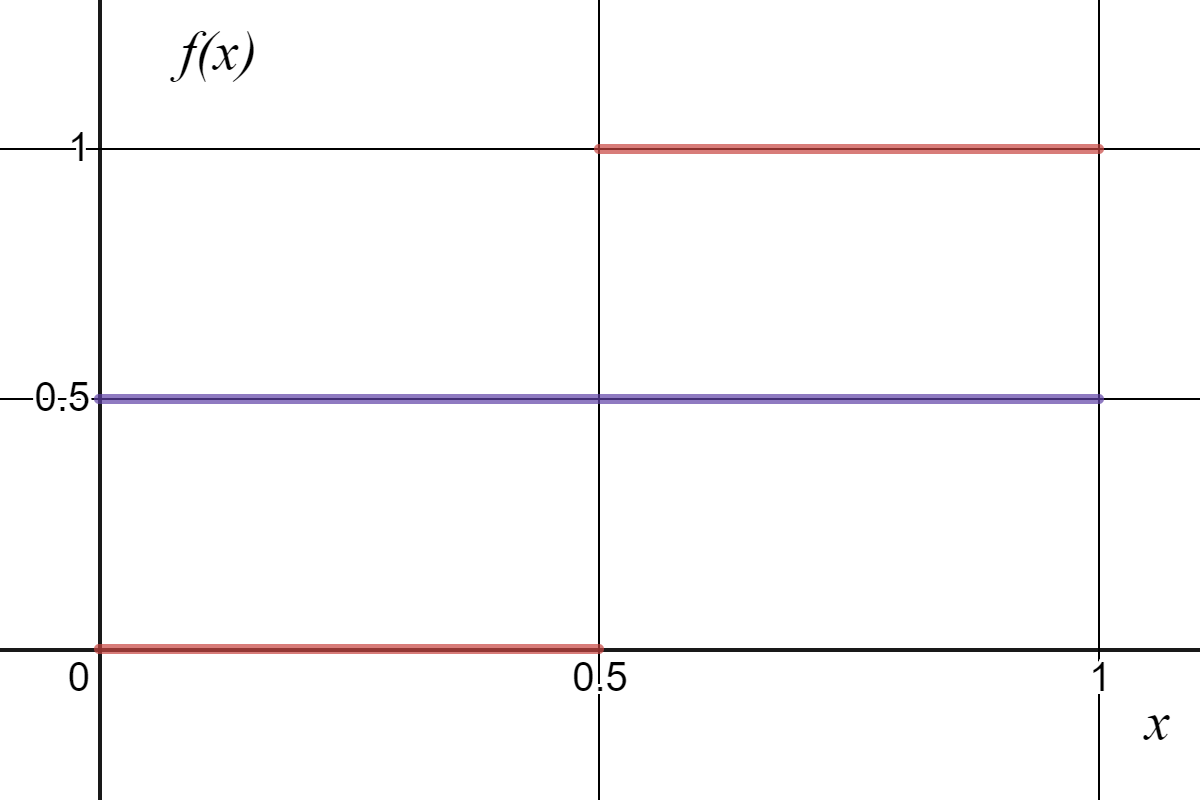
\includegraphics[width=\textwidth]{Figures_Part_5/N=0.png}
				\caption{$N=0$ approximation.}
			\end{subfigure}
			~ 
			\begin{subfigure}[h]{0.3\textwidth}
				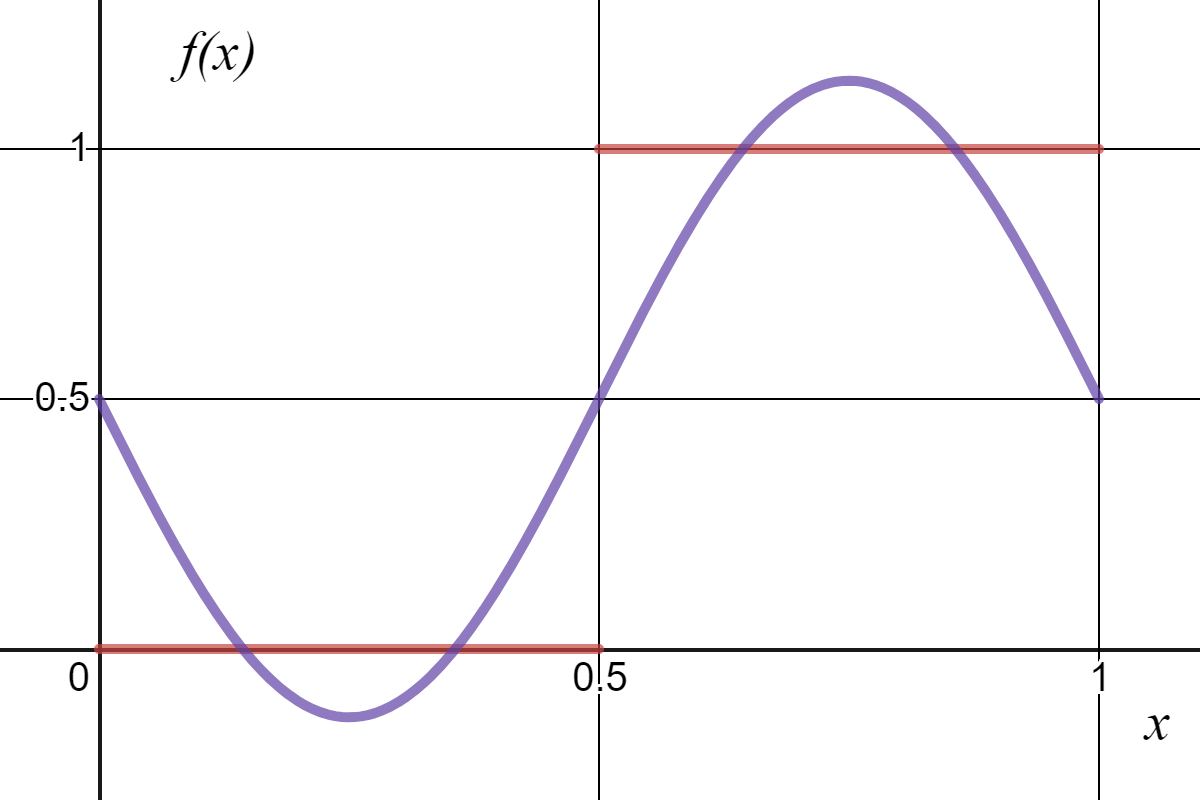
\includegraphics[width=\textwidth]{Figures_Part_5/N=1.png}
				\caption{$N=1$ approximation.}
			\end{subfigure}
			~
			\begin{subfigure}[h]{0.3\textwidth}
				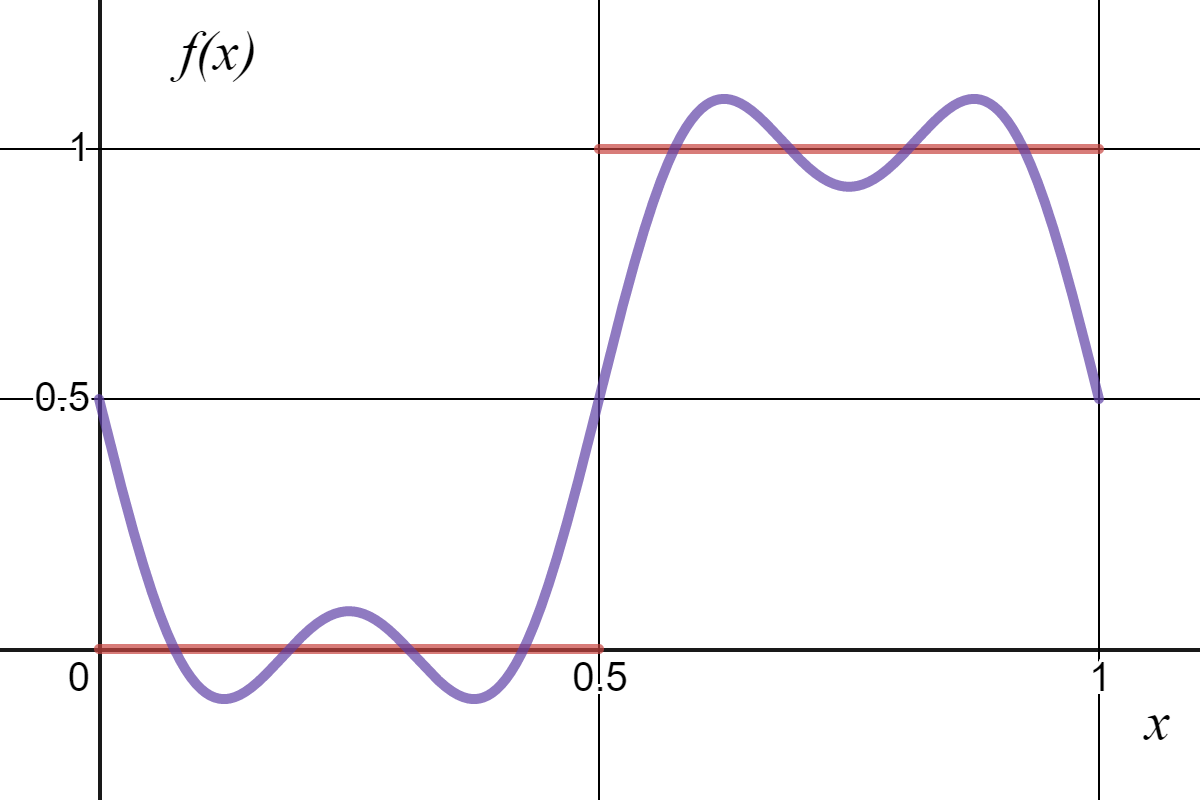
\includegraphics[width=\textwidth]{Figures_Part_5/N=3.png}
				\caption{$N=3$ approximation.}
			\end{subfigure}\\
			
			\begin{subfigure}[h]{0.3\textwidth}
				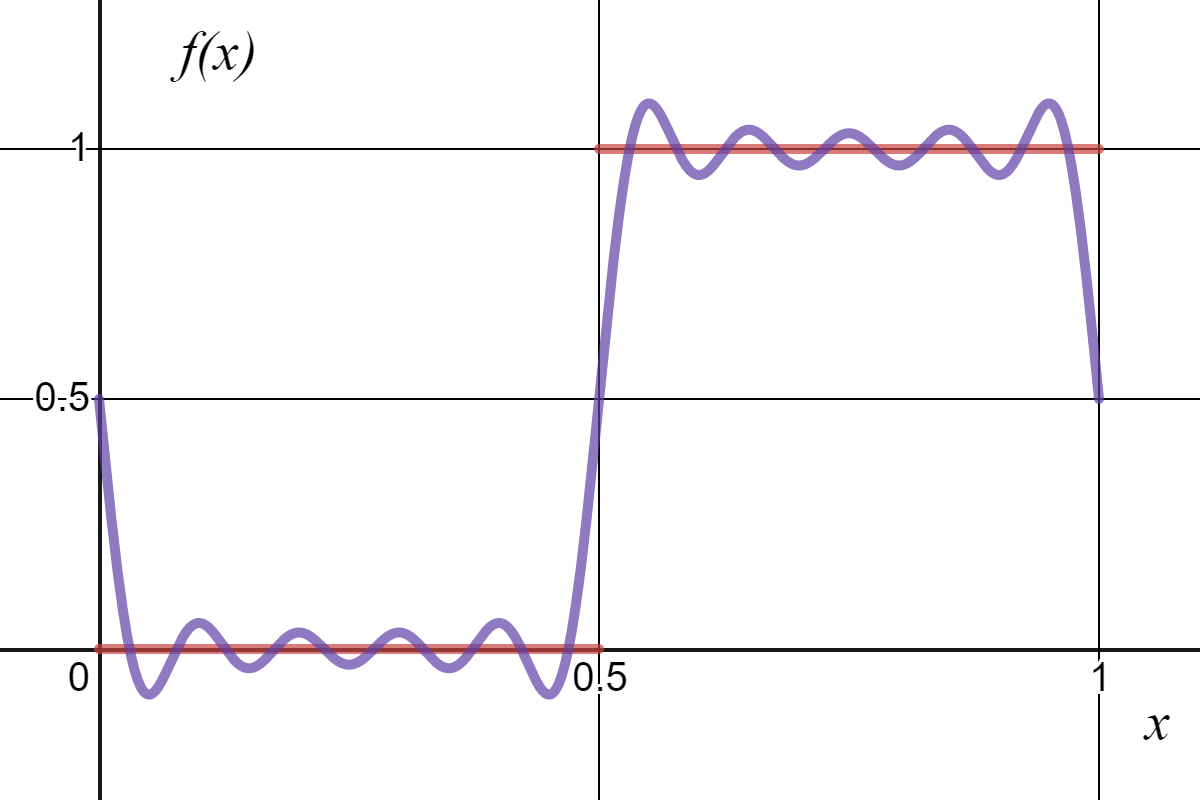
\includegraphics[width=\textwidth]{Figures_Part_5/N=10.png}
				\caption{$N=10$ approximation.}
			\end{subfigure}
			~ 
			\begin{subfigure}[h]{0.3\textwidth}
				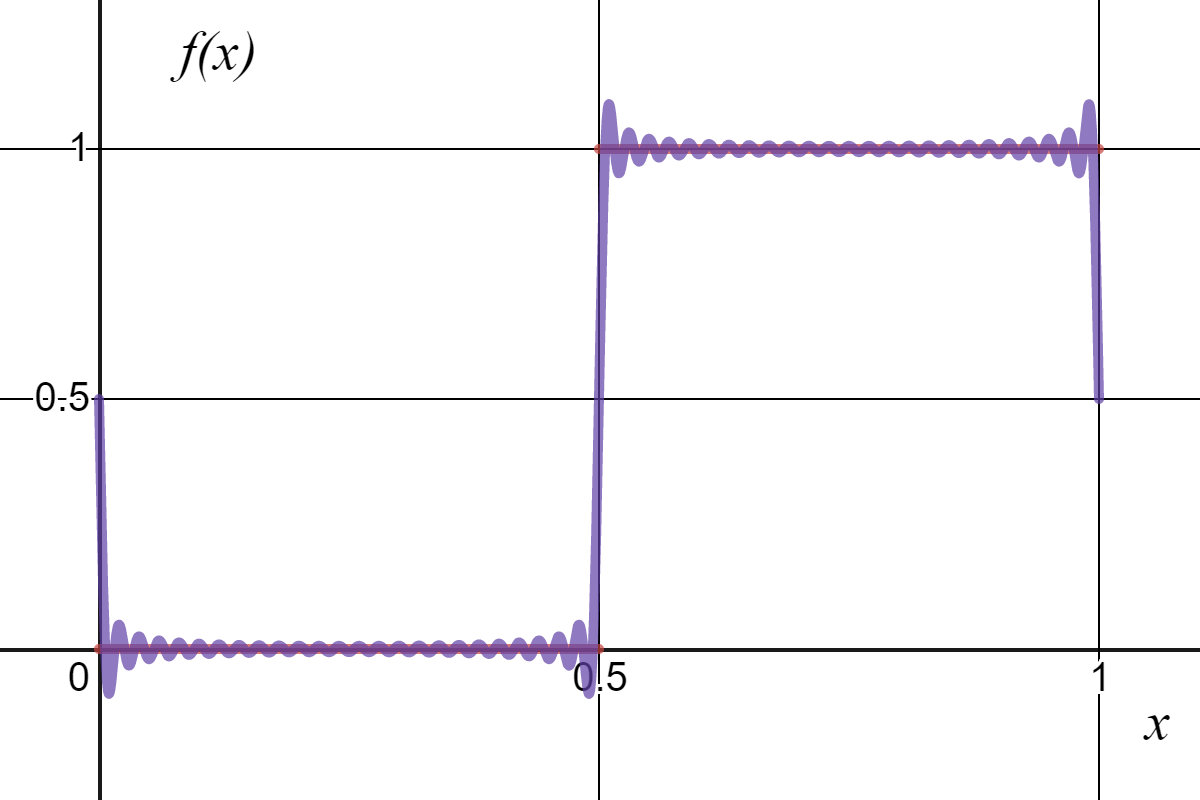
\includegraphics[width=\textwidth]{Figures_Part_5/N=50.png}
				\caption{$N=50$ approximation.}
			\end{subfigure}
			~
			\begin{subfigure}[h]{0.3\textwidth}
				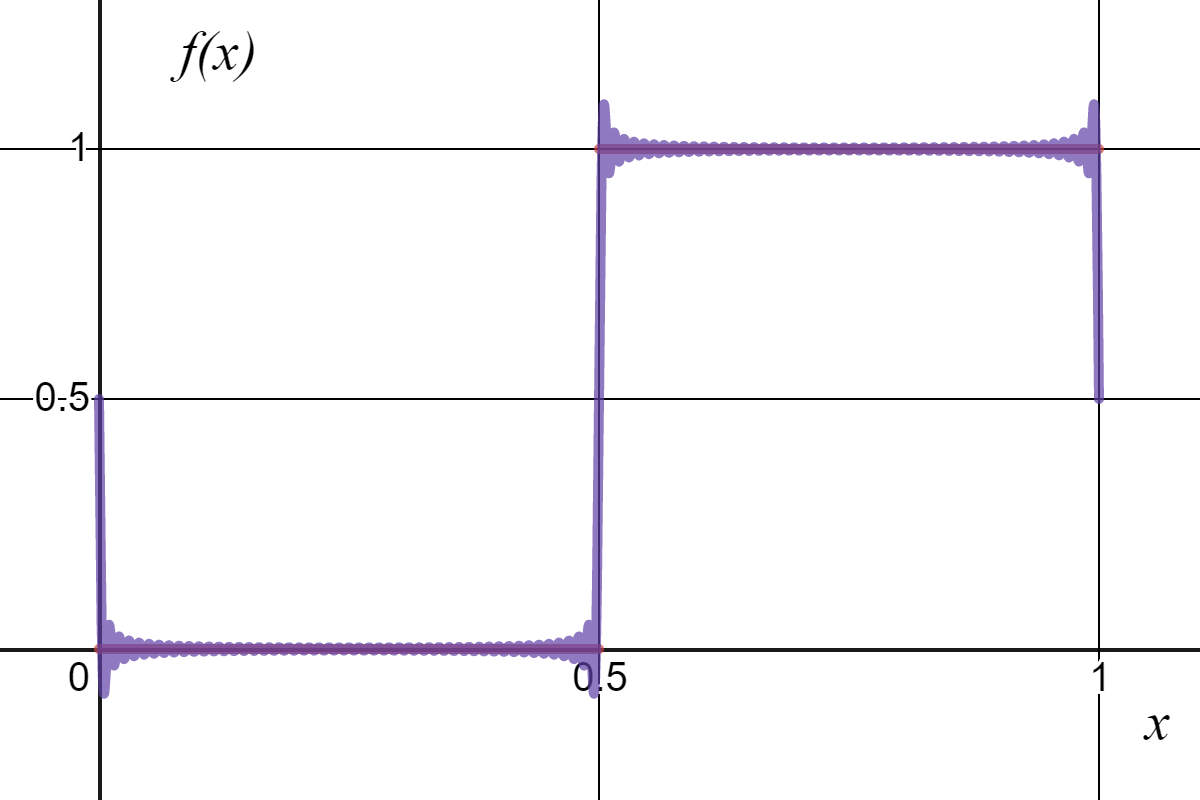
\includegraphics[width=\textwidth]{Figures_Part_5/N=100.png}
				\caption{$N=100$ approximation.}
			\end{subfigure}
		\caption{True $f(x)$ in red. Approximations in purple.}
		\end{figure}
\end{ex}

\section{Fourier Transform}

Let us transition into a more general point of view of the Fourier series.  Specifically, we wish to utilize the Fourier transform.  The idea behind the Fourier transform is to convert a given function $f$ into a new one that we denote by $\hat{f}$ that contains the frequency information of $f$.  This new function will look different, but it will be (in some way) equivalent to our original function. However, we do gain some ability to solve differential equations with the transformed function. 

First, we can rewrite the Fourier series by using complex functions.  Again, we consider functions defined on the interval $[0,L]$ and take the functions
\[
e^{\frac{i 2n \pi x}{L}} \qquad n=\dots, -2,-1,0,1,2,\dots,
\]
as our orthonormal basis functions.  Note that these are indeed normalized when we take the inner product
\begin{align*}
\innprod{e^{\frac{i 2n \pi x}{L}}}{e^{\frac{i 2n \pi x}{L}}} &= \frac{1}{L} \int_0^Le^{\frac{i 2n \pi x}{L}}e^{\frac{-i 2n \pi x}{L}}dx\\
&= \frac{1}{L}\int_0^L 1 dx\\
&= 1.
\end{align*}
In some way we can now see that the functions are a bit more natural to use.  Recall of course that Euler's formula gives us the connection from this representation to the one we previously discussed. That is,
\[
e^{\frac{i 2n \pi x}{L}} = \cos\left(\frac{2n \pi x}{L}\right) + i \sin\left(\frac{2 n \pi x}{L} \right).
\]
Thus, we can write functions by taking the following linear combination
\[
f(x) = \sum_{-\infty}^\infty c_n e^{\frac{i 2n \pi x}{L}},
\]
where the constants $c_n$ are allowed to be complex valued.  Then, the \boldgreen{Fourier transform} of the function $f$, denoted by $\hat{f}$, is given by
\[
\hat{f}(k) = c_k,
\]
is the coefficients of from the Fourier series.  Thus, what we find is that the Fourier transform describes ``how much" of the frequency $\frac{2 k \pi}{L}$ makes up the function $f$.

\begin{ex}{Square Wave Fourier Transform}{square_wave_transform}
	If we consider the square wave function given by
	\[
	f(x) = \begin{cases} 0 & x<L/2 \\ 1 & x\geq L/2, \end{cases},
	\]
	then we can compute the Fourier components with the complex basis functions
	\[
	e^{\frac{ i 2n \pi x}{L}}.
	\]
	Thus, we compute the coefficients in the same by
	\begin{align*}
		c_k &= \innprod{f}{e^{\frac{ i 2n \pi x}{L}}}\\
		&= \frac{ie^{i \pi k}(-1-e^{i\pi k})}{2\pi k}\\
		&= \frac{i(-1)^k (-1-(-1)^k)}{2\pi k}\\
	\end{align*}
	Hence, the Fourier transform of $f$ is given by
	\[
	\hat{f}(k) =  \frac{i(-1)^k (-1-(-1)^k)}{2\pi k}.
	\]
\end{ex}

We'll arrive at the usefulness of the Fourier transform in a bit, but we will first want to consider a yet more general version of the Fourier transform. Instead of taking functions defined solely on the interval $[0,L]$, we can create a transform that works for functions defined on all of $\R$ or any subset.  The difference is this: we now take a basis of functions to be
\[
e^{i2\pi k x} \qquad k \in \R.
\]
That is, instead of taking a discrete set of basis functions, we will now need a continuous set of basis functions.  The reason for this, heuristically, is due to the fact that there can be a full continuum of frequencies for functions defined on $\R$.  The details are suitably more involved than we can get into for a course at this level!

One may now see why we have built up this framework in the way that we did.  It was a bit of a drawn out process, but it allows us to compute the Fourier transform in a consistent way.  Given a function $f(x)$, we can define the Fourier transform by taking the Hermitian inner product for $\R$ and projecting our function onto the basis elements. For example, we have
\[
\hat{f}(k) = \innprod{f}{e^{i2\pi k x}} = \int_{-\infty}^\infty f(x)e^{-i2\pi kx}dx.
\]
And that's really all!  However, one must mention an immensely important function before we compute some examples.

\subsection{Fourier Transform Operator}

Often time, it will be useful to talk of the Fourier transform as an operator. For this, we will use the notation
\[
\fourier{f(x)}= \hat{f}(k).
\]
Later, we will introduce the inverse operation in that 
\[
\fourierinv{\hat{f}(k)}=f(x).
\]
These operators are fundamental in solving differential equations!

One should also note that the Fourier transform is a unitary linear operator.  Specifically, if we have two functions $f$ and $g$ and a constant $\alpha\in \C$, then
\[
\fourier{f(x)+\alpha g(x)} = \hat{f}(k)+\alpha \hat{g}(k).
\]
Now, the operator is unitary since we also have that
\[
\innprod{f}{g} = \innprod{\hat{f}}{\hat{g}},
\]
where the integrals used to evaluate the inner products are taken over the variables $x$ and $k$ respectively.  

The fact that the Fourier transform is a unitary operator is rather important. It means that the transformation does not disturb the measurements one could wish to make. In the same vein, it allows one to work with the transformed function $\hat{f}(k)$ without losing any information about the system. We'll find that working with $\hat{f}(k)$ is often an easier task.

\section{The Dirac Delta Function}

Studying the Fourier theory naturally brings about a very special (generalized) function known as the \boldgreen{Dirac delta function} which we denote by $\delta(x)$.  Quite simply, we define this function via an integral. Specifically, we have for any function $f(x)$ that
\[
\int_{-\infty}^\infty f(x)\delta(x) dx = f(0).
\]
Moreover, if the interval $[a,b]$ contains $0$, we have
\[
\int_a^b f(x)\delta(x) dx = f(0).
\]
We can change the input value for $\delta(x)$ by taking $\delta(x-x_0)$ and we have
\[
\int_{-\infty}^\infty f(x)\delta(x-x_0)dx = f(x_0).
\]
Put in more simple terms, $\delta$ is the function that, when integrated with another function $f$, evaluates that function at a given input value (so long as we integrate over that input value).  

\begin{remark}
	$\delta(x)$ is in fact \underline{not} a function at all. It is something more general known as a distribution. But this fact is not entirely relevant. We will continue to refer to $\delta(x)$ as a function despite this slight misnomer.
\end{remark}

Why should one even consider such a function? For one, it will show up quite readily for us when using the Fourier transform. But, moreover, it is a physically meaningful function in that describes a concentration of mass at a single point.  For example, when studying electromagnetism, one will talk of charged particles. Often, those charged particles are thought of as single points with a charge $q$.  To determine the total charge in a region, one would perform an integral like
\[
\int_{-\infty}^\infty q\delta(x)dx = q
\]
which shows the total charge $q$. The fact that we have $q\delta(x)$ tells us that all of the charge is concentrated at $x=0$.  

One can define the delta function in another convenient manner.  Specifically, via the Fourier transform. One can also show that 
\[
\delta(x) = \int_{-\infty}^\infty 1 e^{-i2\pi kx}dx, 
\]
which means that the $\delta$ function is the Fourier transform of the constant function.  Moreover,
\[
c\delta(x) = \int_{-\infty}^\infty c e^{-i2\pi kx}dx.
\]
One should believe this on an intuitive level since the Fourier transform of a function returns the function's frequency components. A constant function has only a zero frequency component and hence the transform must reflect this.  

\begin{remark}
	Computing these integrals requires tools from complex analysis that we have not seen.  Thus, we will have to blackbox how these integrals are computed in exchange for their usefulness.
\end{remark}

\section{Computing Fourier Transforms}

To see what we are working with, we should compute a few examples. Once again, the techniques to compute these integrals are beyond the scope of this text, but we can show a few results anyways. Our first goal is to see what is meant by frequency components of a function.

If we start with functions with a constant period of oscillation, we can try to digest what the output of the Fourier transform is telling us. We will consider three functions, each with the same period, and compare their transforms.

\begin{ex}{Fourier Transform of Cosine}{fourier_transform_cosine}
	Let us consider the Fourier transform of the function $f(x)=\cos(x)$.  We can compute this transformation by
	\begin{align*}
	\fourier{f(x)} &= \int_{-\infty}^\infty \cos(x)e^{i2\pi kx}dx\\
	&= \frac{\delta\left(k-\frac{1}{2\pi}\right)-\delta\left((k+\frac{1}{2\pi}\right)}{2}.
	\end{align*}
	Here, we can see that the recovered frequency components are where the input to the delta functions are zero. That is,
	\[
	-2\pi k -1 = 0~ \implies ~k= -\frac{1}{2\pi},
	\]
	and
	\[
	1-2\pi k = 0~ \implies ~k=\frac{1}{2\pi}.
	\]
	Recall that the period of $\cos(x)$ is $2\pi$ and hence the frequency $\nu = \frac{1}{2\pi}$. Here, we can see that there is both a $\pm \frac{1}{2 \pi}$.
\end{ex}

In the previous example, one can see how the Fourier transform breaks the function down into frequency components. However, we also know of another function whose frequency is $2\pi$. Namely, $\sin(x)$. Note that these functions are different in that $\cos(x)$ is an even function and $\sin(x)$ is an odd function, so we should expect their Fourier transforms to differ as well (or else this is not an invertible process).

\begin{ex}{Fourier Transform of Sine}{fourier_transform_sine}
	Similarly, we could consider the Fourier transform of the function $f(x)=\sin(x)$.  We'll take
	\begin{align*}
		\fourier{f(x)} &= \int_{-\infty}^\infty \sin(x) e^{i2\pi kx} dx\\
		&= \frac{\delta\left(k-\frac{1}{2\pi}\right)-\delta\left(k+\frac{1}{2\pi}\right)}{2i}
	\end{align*}
	What we see is that the constants in front of the delta functions are different for $\sin(x)$. Specifically, we see the inclusion of the imaginary unit $i$. 
\end{ex}

The differences above display how the Fourier transform is capturing more information about a function than just the frequency information. In some sense, the Fourier transform can determine how even or odd a function is as well.  To finalize this section, let us consider the Fourier transform of another function with frequency $\frac{1}{2\pi}$.

\begin{ex}{Fourier Transform of Complex Exponential}{fourier_transform_exponential}
	Let $f(x)= e^{ix}$, and note that this function has a period of $2\pi$ and hence a frequency of $\frac{1}{2\pi}$.  We can also recall that by Euler's formula, we have
	\[
	e^{ix} = \cos(x)+i\sin(x),
	\]
	and thus we can compute the Fourier transform by
	\begin{align*}
		\fourier{e^{ix}} &= \fourier{\cos(x)+i\sin(x)}\\
		&= \fourier{\cos(x)}+i\fourier{\sin(x)}\\
		&= \delta\left(k-\frac{1}{2\pi}\right)
	\end{align*}
	Again, we find that the Fourier transform captures enough information about our functions to properly differentiate between them.  
\end{ex}

This section would not be complete without some reference of common Fourier transforms.  We'll place a few here, but there are many other references to compute more examples (see for example Wikipedia's page on \emph{Tables of Important Fourier Transforms}.

\begin{table}[H]
        \centering
        \renewcommand{\arraystretch}{2}
        \begin{tabular}{c|c}
            $f(x)$ & $\hat{f}(k)$\\
            \hline
         	$\delta(x)$ & $1$\\
         	$1$ & $\delta(x)$\\
         	$e^{iax}$ & $\delta\left(k-\frac{a}{2\pi}\right)$\\
         	$\cos(ax)$ & $\frac{\delta\left(k-\frac{a}{2\pi}\right)+\delta\left(k+\frac{a}{2\pi}\right)}{2}$\\
     		$\sin(ax)$ & $\frac{\delta\left(k-\frac{a}{2\pi}\right)-\delta\left(k+\frac{a}{2\pi}\right)}{2i}$
        \end{tabular}
        \label{tab:fourier_transform}
    \end{table}
    
\section{The Inverse Fourier Transform}

The most striking property of the Fourier transform is that it is invertible. Coupled with its linear and unitary nature, the Fourier transform has many nice properties that allow one to make great use of it.  Up until this point, we have only dealt with the forward direction of the Fourier transform. If we are given a function $f(x)$, we can convert this function into $\hat{f}(k)$ which we refer to as the transformed function in the \boldgreen{frequency domain}.  We put
\[
\fourier{f(x)}=\hat{f}(k).
\]
Now, the claim is that this process is invertible in that if we are given a function $\hat{f}(k)$ in the frequency domain, we can convert it back to a function $f(x)$.  That is, we want 
\[
\fourierinv{\hat{f}(k)} = f(x).
\]
Now, since the Fourier transform is a unitary operator, we need only find the adjoint to the Fourier transform.  Recall that, given a unitary operator $\unitop$ we can find $\unitop^{-1}$ by solving
\[
\unitop \unitop^{-1} = I,
\]
where $I$ is the identity. However, the defining property of a unitary operator is that we have
\[
\unitop^{-1} = \unitop^\dagger.
\]
That is, the inverse of a unitary operator is its adjoint! 

Hence, it follows that the \boldgreen{inverse Fourier transform} of a function $\hat{f}(k)$ is given by
\[
f(x) = \int_{-\infty}^\infty \hat{f}(k) e^{i2\pi kx}dk.
\]
If one revisits example \ref{ex:phase_operator}, then we can see that the adjoint to multiplication by a phase is to multiply by the negative phase. That is, the adjoint to $e^{i\theta}$ is $e^{-i\theta}$.  That is the fact that lets us define the inverse Fourier transform above. 

In \ref{tab:fourier_transform}, one can find the inverse Fourier transform of a given function by starting with a $\hat{f}(k)$ and seeing what the corresponding $f(x)$ is.  We'll not worry so much about inverting other functions for now.  

\section{Solving Differential Equations}

Perhaps the most unique feature of the Fourier transform is the transformation of derivatives of a function.  One could in fact argue that this was the true nature of the transformation from the beginning.  Consider a function $f(x)$, then we can differentiate $f(x)$ to get the function $f'(x)$. Now, what is the Fourier transform
\[
\fourier{f'(x)}?
\]
First, (though we have yet to mention this) let us note that any $f(x)$ must be a function that decays rapidly as $x\to \pm \infty$. Let's write this out. We have
\begin{align*}
	\fourier{f'(x)} &= \int_{-\infty}^\infty f'(x)e^{-i2\pi kx}dx\\
	&= i2\pi k \int_{-\infty}^\infty f(x) e^{i2\pi kx}dx\\
	&= i2\pi k \hat{f}(k).
\end{align*}

\begin{exercise}
	Using integration by parts, show that the work above is correct. 
\end{exercise}

What we have found is that the Fourier transform turns derivatives into a multiplication operator! This can be summed up in the following way:
\[
\boxed{\fourier{\frac{d^n}{dx^n} f(x)} = (i2\pi kx)^n \hat{f}(k).}
\]

We also have the following as well
\[
\boxed{\fourier{x^n f(x)} = \left(\frac{i}{2\pi}\right)^n \frac{d^n}{dk^n} \hat{f}(k).}
\]
This means that the Fourier transform turns multiplication into differentiation.  

What follows is an algebraic method for solving differential equations. Specifically, any linear differential equation can be quickly transformed into a new (possibly easier) differential equation. The outline can be summarized in the following steps.
\begin{enumerate}[1.]
	\item Take a Fourier transform of both sides of your differential equation.
	\item Solve the new equation for $\hat{f}(k)$ in terms of the frequency variable $k$.
	\item Use the inverse Fourier transform to convert $\hat{f}(k)$ back to $f(x)$.
\end{enumerate}

We'll first start with an example that uses the Fourier series as opposed to the Fourier transform.  Underlying the solution is the same principal, but it gives us a better means for understanding the methodology.

\begin{ex}{Fourier Series/Transform Solution of a Second Order Equation}{fourier_transform_first_order}
	Consider an elastic band suspended from atop two poles subject to the force of gravity. We can model this equation by
	\[
	-k\frac{d^2}{dx^2}(x) = g(x),
	\]
	with the boundary conditions $f(0)=f(L)=0$. Here, $k$ is an elastic constant that describes the stiffness of the elastic.  Then, we let 
	\[
	g(x) = \begin{cases} 0 & x<L/4 \\ 1 & L/4 \leq x < 3L/4 \\ 0 & 3L/4<x \end{cases},
	\]
	which has the following graph.
	\textcolor{red}{add figure}
	Let us suppose that $f(x)$ is written as a Fourier series,
	\begin{align*}
		f(x) = ...
	\end{align*}
	
	Then do fourier transform with complex exponentials version to lead into fourier transform. 
	
\end{ex}
	



%\part{Calculus in Higher Dimensions}
%
%\chapter{Curves and Fields}
%   
        \section{Overview of multivariate functions}
        Aside from the study of linear transformations on $\R^n$ or $\C^n$, we have limited ourselves to functions of a single variable.  Given that we have performed a deep analysis for functions of one variable, we can take what we have learned and apply it to new types of functions. Specifically, we will concentrate on $\R^3$ (or $\R^2$) and functions of the form:
        \begin{align*}
            &\curvegamma\colon \R \to \R^3\\
            &f\colon \R^3 \to \R\\
            &\vecfieldV \colon \R^3 \to \R^3.
        \end{align*}
        Of these three functions, the latter two are often referred to as \boldgreen{fields}.  These are also \boldgreen{multivariate} functions, whereas the first only has an input of a single variable.
        
        
        \begin{enumerate}[(1)]
        \item Functions of the form
        \[
        \curvegamma \colon \R\to \R^3
        \]
        are \boldgreen{curves}.  Often times, we will have 
        \[
        \curvegamma \colon [a,b]\to \R^3
        \]
        when we want curves with specific endpoints. We will concentrate first on curves, so I'll save the extra detail for a bit later.
        
        \item Functions of the form
        \[
        f\colon \R^3 \to \R
        \]
        are \boldgreen{scalar fields} .   These functions are useful in describing quantities like temperature in space.  In this example, at each point $\vecx$ in space $\R^3$, we can assign a single real number output $f(\vecx)$ that tells us this temperature.  
        
        %One may ask how this function changes from point to point.  Asking this question sends you immediately to investigating the \emph{gradient}.  It turns out, using our temperature example, that we can understand heat flow by understanding temperature gradients.
        
        \item Functions of the form
        \[
        \vecfieldV \colon \R^3 \to \R^3
        \]
        are called \boldgreen{vector fields}.  Roughly speaking, at each point $\vecx$ in space $\R^3$, we can place a vector $\vecfieldV(\vecx)$ that is also in $\R^3$.  These fields are very important in describing systems that have flow.  For example, fluid flow or electromagnetism are vector field theories. 
        
        % What will it mean to find the change in a vector field?  This will lead us to the notion of the \emph{total derivative}.  This concept is a bit abstract at first but will really tell us the proper notion of the derivative.
        \end{enumerate}
        
        
        \section{Curves in space}
        
        We will begin with curves as they are very useful tools and this will help us visualize results for the other types of functions. 
        
        Let us consider a curve
        \[
        \curvegamma \colon \R \to \R^3.
        \]
        We will specify a specific curve by supplying three functions $f_1(t)$, $f_2(t)$, and $f_3(t)$. Specifically, each of these functions $f_i$ is a function $f_i\colon \R \to \R$. Then, we can say that
        \[
        \curvegamma(t)=\begin{pmatrix} \gamma_1(t)\\ \gamma_2(t)\\ \gamma_3(t)\end{pmatrix}.
        \]
       Each $\gamma_i(t)$ (for the values $i=1,2,3$) represents the components of a vector that changes with respect to the variable $t$. Intuitively, we like to think of the components as evolving in time, which is why we make use of the variable $t$. To say this more explicitly, we can write
        \begin{align*}
            &\gamma_1(t) \quad \textrm{the $x$-position of $\gamma$ at time $t$,}\\
            &\gamma_2(t) \quad \textrm{the $y$-position of $\gamma$ at time $t$,}\\
            &\gamma_3(t) \quad \textrm{the $z$-position of $\gamma$ at time $t$.}
        \end{align*}
        
        \begin{ex}{A Planar Curve}{planar_curve}
        	We briefly covered the notion of curves when we considered complex valued functions.  Here, we can liken a planar curve $\curvegamma$ to a complex valued function with a real valued input.  For example, let us take a curve $\curvegamma \colon [0,1] \to \R^2$ by
        	\[
        	\curvegamma = \begin{pmatrix} t \\ t \end{pmatrix}.
        	\]
        	This gives us the components
        	\[
        	\gamma_1(t) = t \qquad \textrm{and} \qquad \gamma_2(t) = t.
        	\]
        	We can plot this curve in the plane by plotting the vector for each time $t$. This gives us
        	\begin{figure}[H]
        		\centering
        		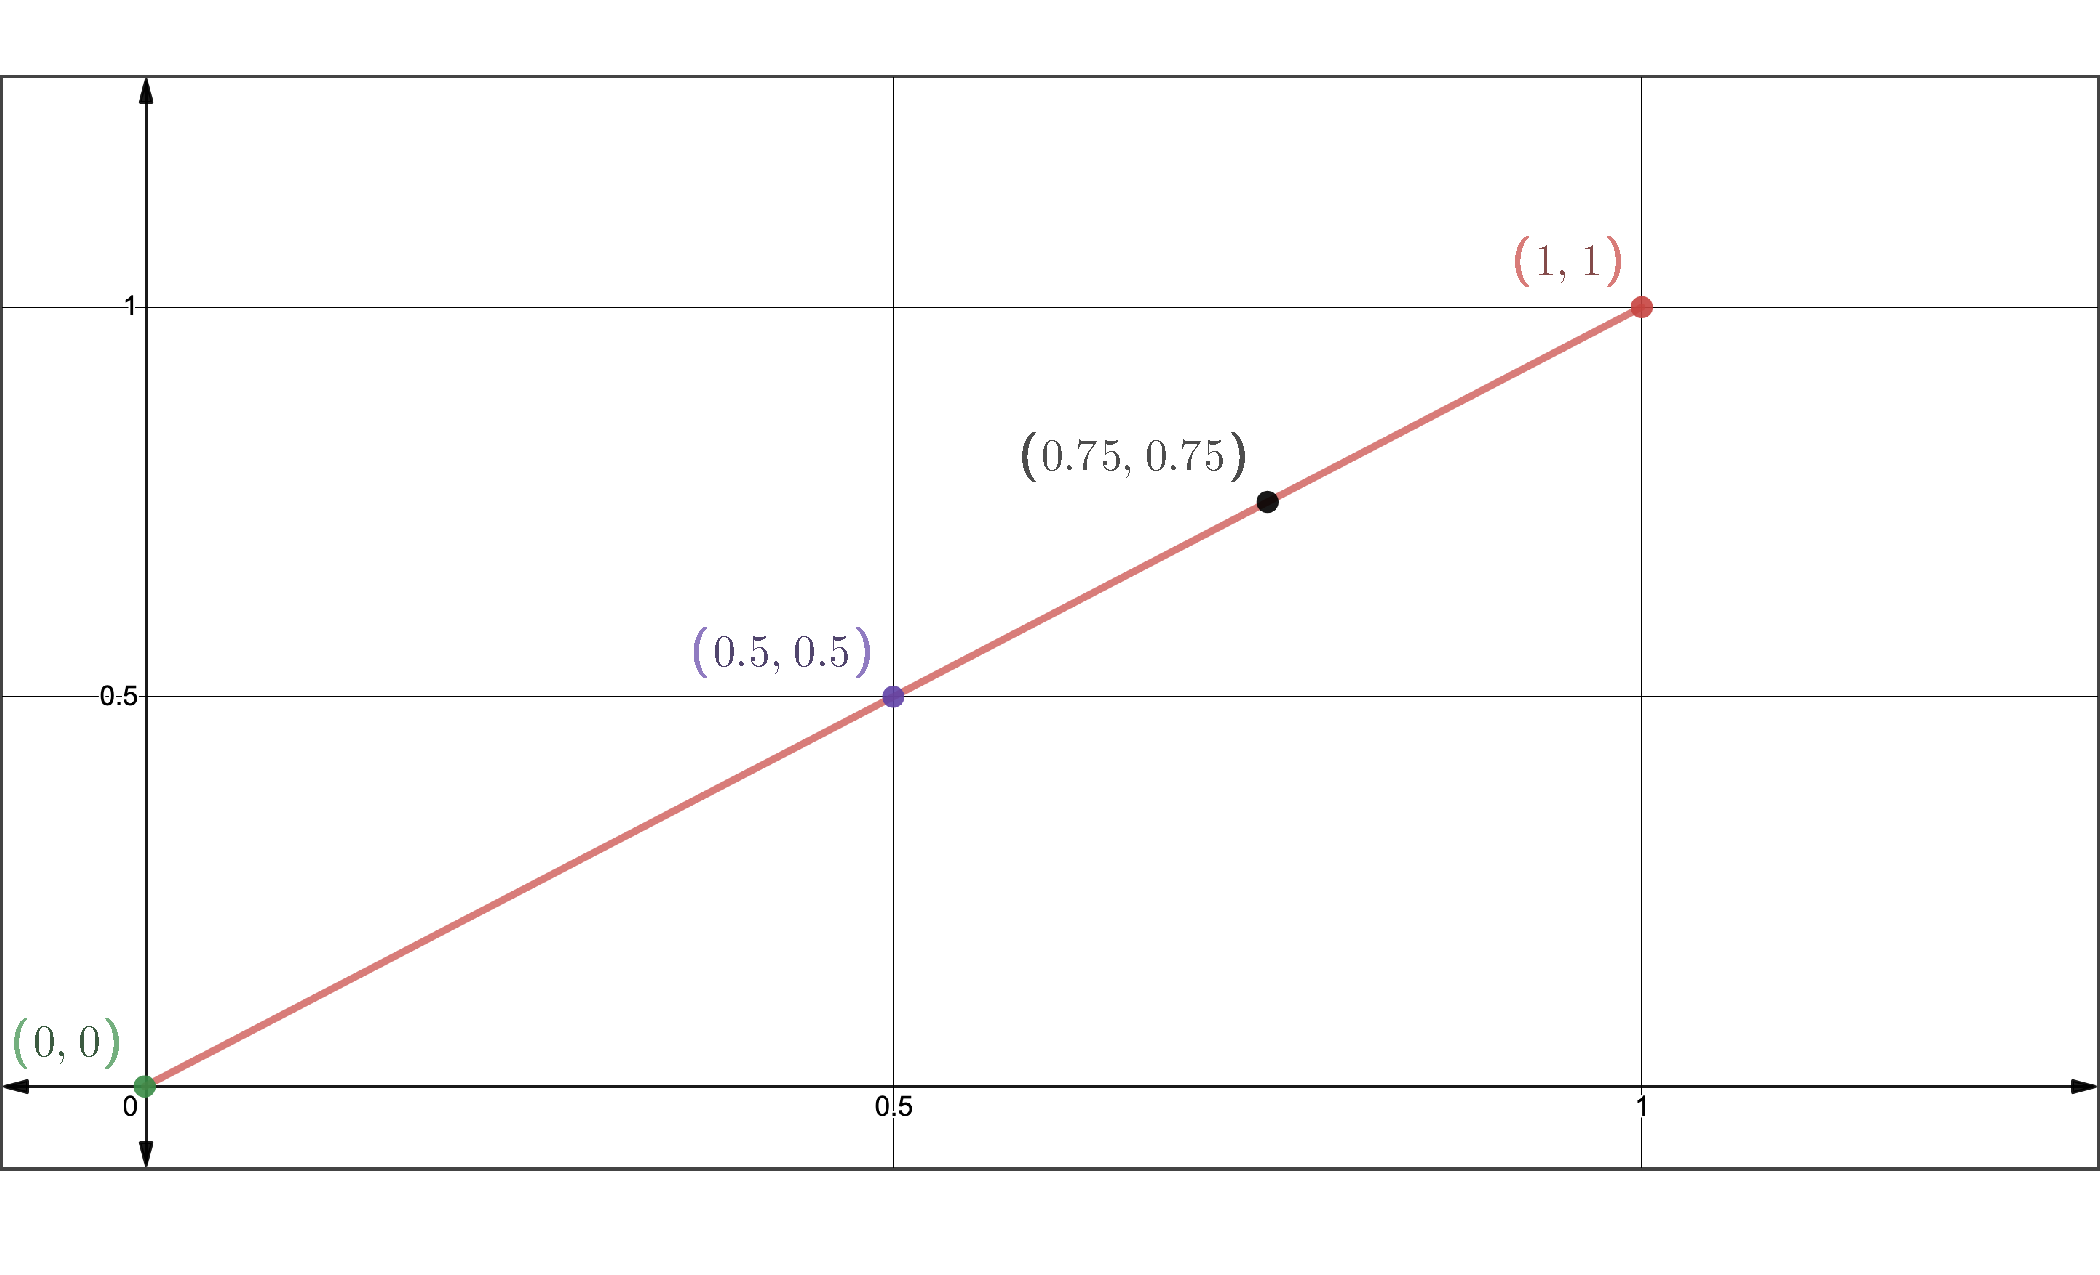
\includegraphics[width=.9\textwidth]{Figures_Part_6/straight_line_curve.pdf}
        		\caption{The curve $\curvegamma(t)$ with labeled points at different times.}
        	\end{figure}
        	In this picture, we can see that the curve begins at the the origin and ends at the point $(1,1)$.  Specifically, we have
        	\[
        	\curvegamma(0) = \begin{pmatrix} 0 \\ 0 \end{pmatrix} \qquad \textrm{and} \qquad \curvegamma(1) = \begin{pmatrix} 1 \\ 1 \end{pmatrix}.
        	\]
        	This curve does not extend indefinitely as our input values can only take on the values in $[0,1]$.
        \end{ex}
        
        From the example, we can see that curves also have a direction associated to them.  As we increase the parameter $t$, we move along the curve in a certain way.  This is an important concept! We can use curves to describe the motion of an object (or other quantities) over time.  This also brings to mind the notion of velocity or speed for a curve.  
        
        \subsection{Derivatives of Curves}
        
        The nice thing about curves is that each component function is a function $\gamma_i\colon \R \to \R$. This means that we can compute the derivatives of each component with the knowledge we have from single variable calculus. In fact, the derivative of a curve can be computed using the typical difference quotient that we learn in a first semester calculus course.  
        
        Imagine that a curve $\curvegamma(t)$ describes the position of a particle at the time $t$.  Then, one could ask for the velocity of this curve which is the first time derivative of position.  Here, we can compute this first derivative at the time $t$ by
        \[
        \tangentgamma(t) = \lim_{\Delta t \to 0} \frac{\curvegamma(t+\Delta t)-\curvegamma(t)}{\Delta t}.
        \]
        We use the overdot notation for $\tangentgamma$ to represent a time derivative of the curve.  We then refer to $\tangentgamma(t)$ as the \boldgreen{tangent vector} to the curve $\curvegamma$ at a time $t$. Now, let us compute the tangent vector explicitly.  We take
        \begin{align*}
        	\tangentgamma(t) &= \lim_{\Delta t \to 0} \frac{\curvegamma(t+\Delta t)-\curvegamma(t)}{\Delta t}\\
        	&= \lim_{\Delta t \to 0} \frac{1}{\Delta t} \left( \begin{pmatrix} \gamma_1(t+\Delta t) \\ \gamma_2(t+\Delta t) \\ \gamma_3(t+\Delta t) \end{pmatrix} - \begin{pmatrix} \gamma_1(t) \\ \gamma_2(t) \\ \gamma_3(t) \end{pmatrix}\right)\\
        	&= \lim_{\Delta t \to 0} \begin{pmatrix} \frac{ \gamma_1(t+\Delta t)-\gamma_1(t)}{\Delta t} \\ \frac{ \gamma_2(t+\Delta t)-\gamma_2(t)}{\Delta t} \\ \frac{ \gamma_3(t+\Delta t)-\gamma_3(t)}{\Delta t} \end{pmatrix}\\
        	&= \begin{pmatrix} \dot{\gamma_1}(t) \\  \dot{\gamma_2}(t) \\ \dot{\gamma_2}(t) \end{pmatrix}.
        \end{align*}
        What this shows is that the tangent vector to a curve $\curvegamma$ is the vector containing the derivative of the components of $\curvegamma$.  Intuitively, this says that the velocity of the curve is found by computing the rate of change of the $x$-component, $y$-component, and $z$-component of $\curvegamma$. 
        
        \begin{ex}{Graph of a Quadratic Function}{graph_quad}
        Consider the curve $\gamma\colon \R \to \R^2$ given by
        \[
        \curvegamma(t)=\begin{pmatrix} t \\ t^2 \end{pmatrix}
        \]
        This curve looks exactly like the graph of the function $f(x)=x^2$ that we have drawn many times before. 
        \begin{figure}[H]
            \centering
            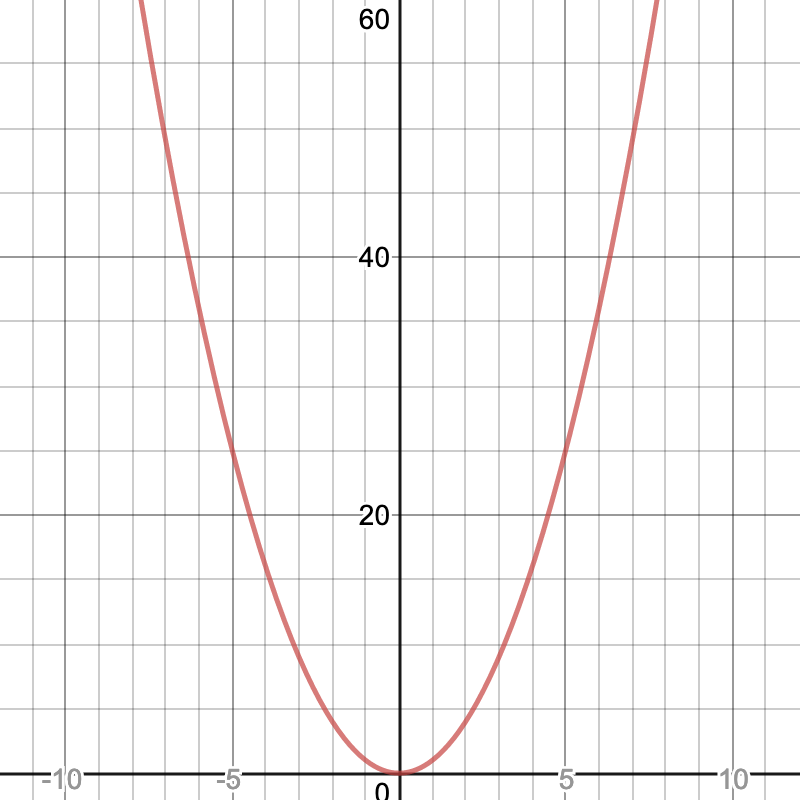
\includegraphics[width=.4\textwidth]{Figures_Part_6/quadratic_curve.png}
        \end{figure}
        What is the tangent vector at time $t$? We have
        \[
        \tangentgamma(t)=\begin{pmatrix} 1 \\ 2t \end{pmatrix}.
        \]
        If we take this $y$-value over the $x$-value we arrive at the same conclusion for the derivative to $f(x)=x^2$ (i.e., $f'(x)=2x$).
        \end{ex}
        
        The two examples of curves we have seen so far mimic graphs of real valued functions we have seen before.  But, curves can be much more general.  There is no need for a curve to pass the horizontal line test, and curves can even have self intersection! For example, a particle that orbits a large body such as the Earth orbits the Sun will move in an elliptical path.  
        
        \begin{ex}{Circle Curve}{circ_curve}
        Consider the curve $\gamma \colon [0,1] \to \R^2$ given by
        \[
        \curvegamma(t)=\begin{pmatrix} \cos (2\pi t) \\ \sin (2\pi t) \end{pmatrix}.
        \]
        This curve is a circle of radius $1$ centered at $(0,0)$.  We can find the tangent vector at a time $t$ by
        \[
        \curvegamma(t)=\begin{pmatrix} -2\pi \sin(2\pi t) \\ 2\pi \cos(2\pi t)\end{pmatrix}.
        \]
        See the following graphs
        
    \begin{figure}[H]
    \centering
    \begin{subfigure}[h]{0.45\textwidth}
        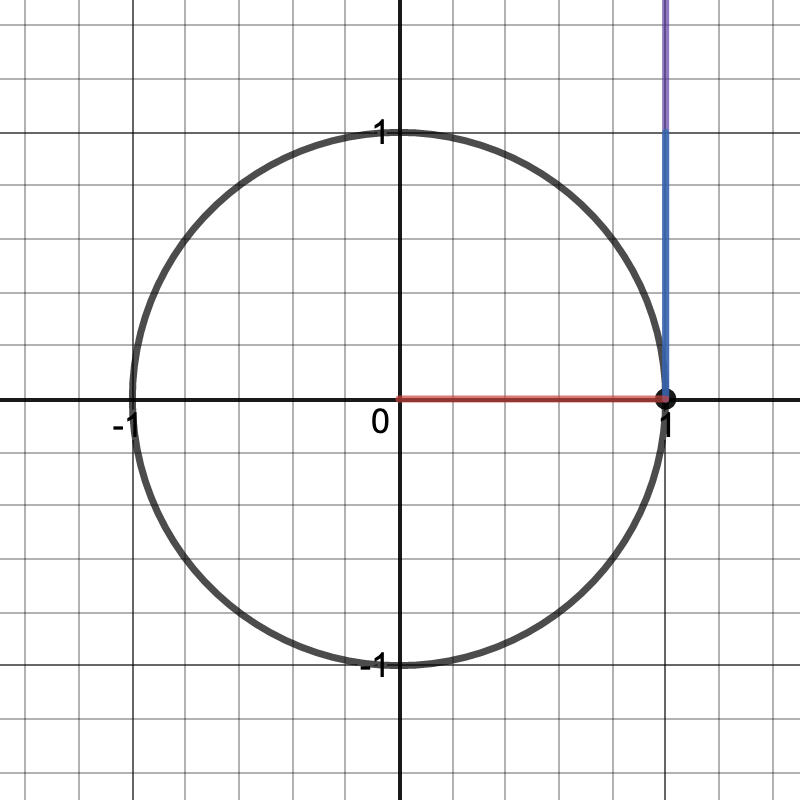
\includegraphics[width=\textwidth]{Figures_Part_6/circ_tang_1.png}
        \caption{Tangent vector at $t=0$.}
    \end{subfigure}
    ~ 
    \begin{subfigure}[h]{0.45\textwidth}
        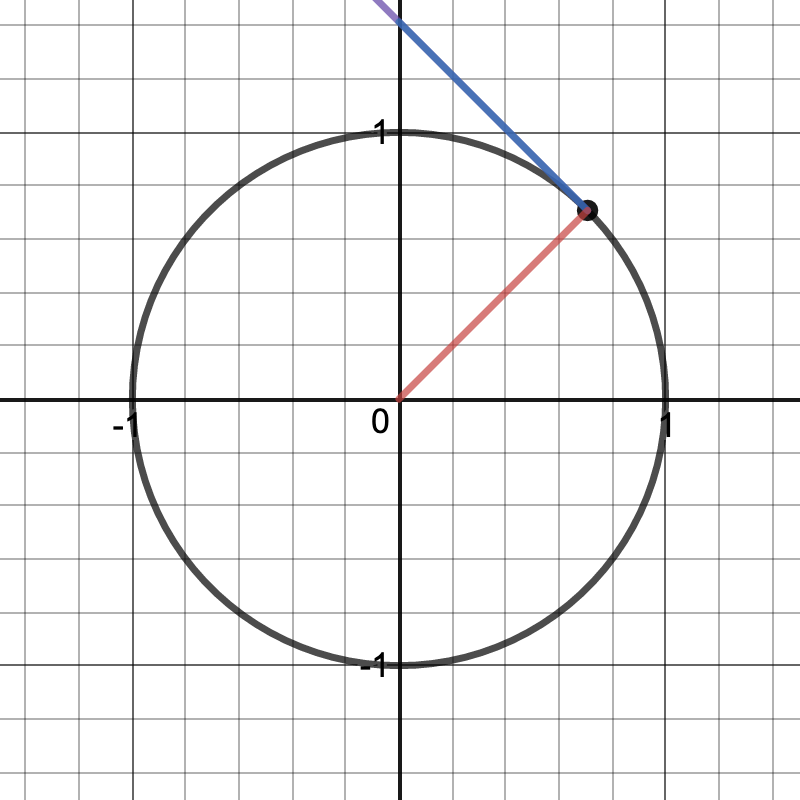
\includegraphics[width=\textwidth]{Figures_Part_6/circ_tang_2.png}
        \caption{Tangent vector at $t=\frac{1}{8}$.}
    \end{subfigure}
    
    \begin{subfigure}[h]{0.45\textwidth}
        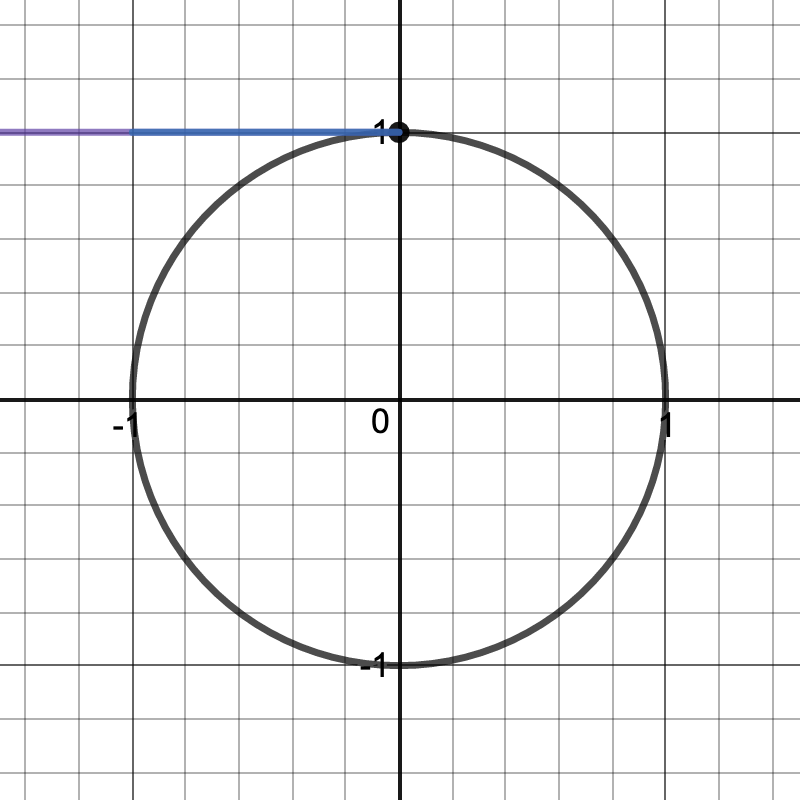
\includegraphics[width=\textwidth]{Figures_Part_6/circ_tang_3.png}
        \caption{Tangent vector at $t=\frac{1}{4}$.}
    \end{subfigure}
    ~
    \begin{subfigure}[h]{0.45\textwidth}
        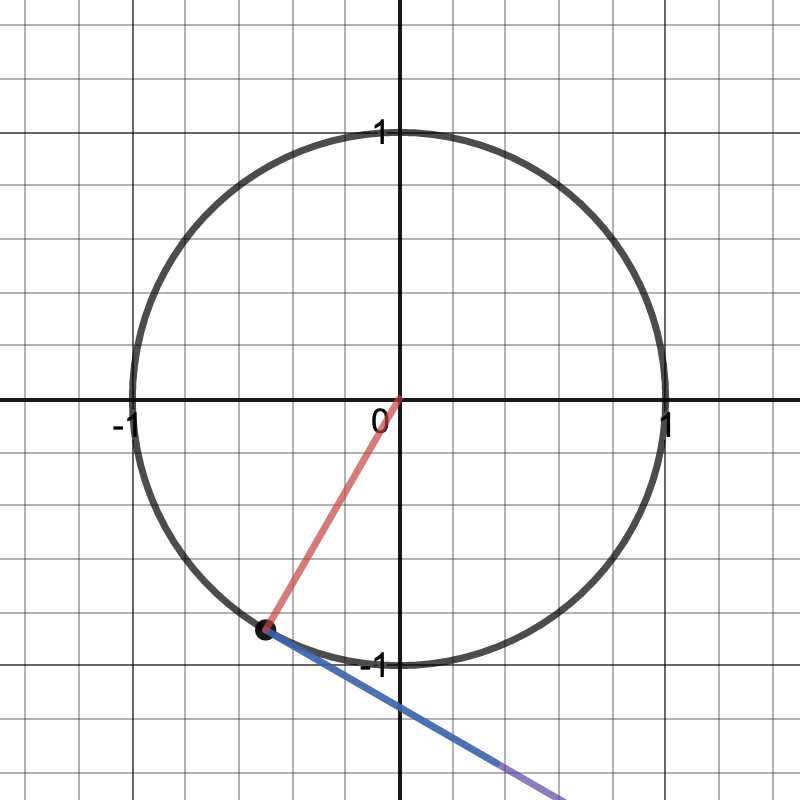
\includegraphics[width=\textwidth]{Figures_Part_6/circ_tang_4.png}
        \caption{Tangent vector at $t=\frac{2}{3}$.}
    \end{subfigure}
        \end{figure}
        \end{ex}
        
        There is nothing stopping us from computing the second time derivative of a curve as well.  We repeat the process for computing the first derivative above, but instead we take the time derivative of the tangent vector $\tangentgamma$.  This yields,
                \[
                \normalgamma(t) = \begin{pmatrix} \ddot{\gamma_1}(t) \\ \ddot{\gamma_2}(t) \\ \ddot{\gamma_3}(t) \end{pmatrix}.
                \]
         We then refer to this quantity as the \boldgreen{normal vector} to the curve $\curvegamma$. 
         
         \begin{exercise}
         	Compute the normal vector to the circle curve in the previous exercise.  If you know of the notion of centripetal force, how does this quantity relate?
         \end{exercise}
         
         \subsection{Lengths of Curves}
        
        Integration is a tool we use to add up values of functions.  In the 1-dimensional case, we found that the integral of a function $f(x)$ from $x=a$ to $x=b$ computed the net area under the graph of the function.  Similarly, we can use integration to compute the length of a curve.
        
        If we take a curve $\curvegamma \colon [a,b] \to \R^3$, then we can compute the tangent vector at time $t$, $\tangentgamma(t)$. Again, the tangent vector is analogous to the velocity of a curve (at some point in time), and so the length of this tangent vector is the speed.  So, we put that the speed of the curve at time $t$ is $\left| \tangentgamma(t)\right|$.  
        
        Computing the length of a curve amounts to adding up the speed of the curve over the total amount of time.  In this perspective, this just takes into account the total distance a particle has moved, even if the particle back-tracks at some point. We can write this length as
        \[
        \ell(\curvegamma) = \int_a^b \left|\tangentgamma(t)\right|dt.
        \]
        
        \begin{ex}{Circumference of a Circle}{circ_of_circ}
        	Take for example the circle curve $\curvegamma \colon [0,1] \to \R^2$ given by
        	\[
        	\curvegamma(t) = \begin{pmatrix} \cos(2\pi t) \\ \sin(2\pi t) \end{pmatrix}.
        	\]
        	Then, we found 
        	\[
        	\tangentgamma(t) = \begin{pmatrix} -2\pi \sin(2\pi t) \\ 2\pi \cos(2 \pi t) \end{pmatrix}.
        	\]
        	Taking the length of the tangent vector at time $t$ yields
        	\[
        	\left| \tangentgamma(t) \right| = \sqrt{4\pi^2 \sin^2(2\pi t) + 4\pi^2 \cos^2(2\pi t) } = 2\pi.
        	\]
        	The length is then
        	\[
        	\ell(\gamma) = \int_0^1 2 \pi t  = 2\pi,
        	\]
        	which is indeed the circumference of a circle of radius one.
        \end{ex}
                
                \section{Scalar fields}
                The next major class of functions we will consider are the scalar fields.  That is, functions that take the form
                \[
                f\colon \R^3 \to \R.
                \]
                Often, it will be helpful to visualize functions by considering instead
                \[
                f\colon \R^2 \to \R
                \]
                and looking at the \boldgreen{graph} of $f$.  
                
                \begin{ex}{Graph of a function}{graph_of_func}
                Whenever we talk of a function of the form
                \[
                f\colon \R \to \R
                \]
                we inherently tend to draw the graph of the function $f$.  By graph, I mean that given $f$, we usually just draw $(x,f(x))$ in the plane.
                
                Take for example, $f\colon \R \to \R$ given by $f(x)=x^2$.  We usually draw the plane $\R^2$ and graph the curve $(x,f(x))$ which looks like
                \begin{figure}[H]
                    \centering
                    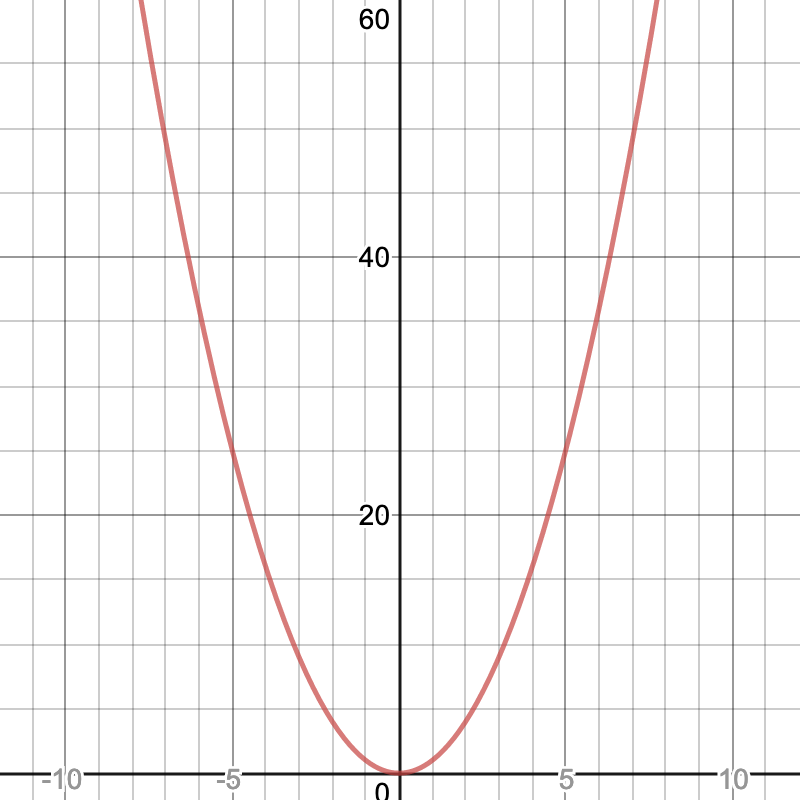
\includegraphics[width=.5\textwidth]{Figures_Part_6/quadratic_curve.png}           
                \end{figure}
                All of this is to say that graphs of these types of functions are special kinds of curves.  In other words, they are curves that pass the vertical line test. 
                \end{ex}
                
                The 1-dimensional examples are rather redundant.  In a vague sense, it's hard to differentiate between 1-dimensional curves, scalar fields, and vector fields.  However, if we consider graphing higher dimensional scalar fields, we will immediately see a difference.  Our new point of view will be to look at the graph of 2-dimensional scalar fields in order to gain intuition on the 3-dimensional scalar fields.  
                
                Graphing a 1-dimensional scalar field $f$ involved plotting the graph
                \[
                (x,f(x)).
                \]
                Here, we put the $y$-component of the output as the function $f(x)$ which allows us to see the function values at a point $x$ as the height above (or below) the $x$-axis. Similarly, if we have a scalar field $h(x,y)$, we can plot the set of points
                \[
                (x,y,h(x,y)),
                \]
                in 3-dimensional space.  Then, what we receive is a picture that places $z=h(x,y)$ so that we see the function $h$ describing the height of a sheet above the $xy$-plane.
                
                \begin{ex}{The Paraboloid}{paraboloid}
                Let $f\colon \R^2 \to \R$ be given by
                \[
                f(x,y)=x^2+y^2.
                \]
                We can plot the graph of the function by plotting $(x,y, f(x,y))$ in $\R^3$.  This will look like:
                \begin{figure}[H]
                    \centering
                    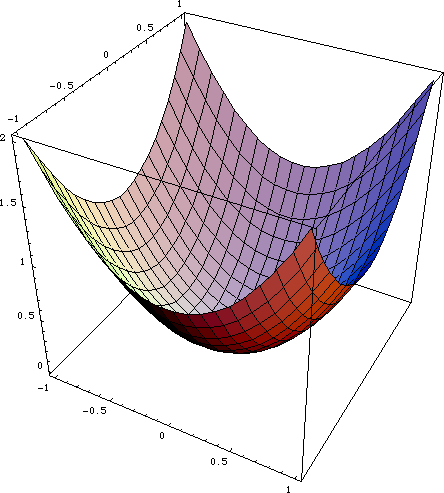
\includegraphics[width=.4\textwidth]{Figures_Part_6/paraboloid.png}
                \end{figure}
                Then we can analyze this function in a few nice ways.  
                
                If we fix a value for $x$ or $y$, then we will be able to look at $f$ as a function of just a single variable.  
                \begin{itemize}
                \item So we can, for example, fix $y=0$ and then we have
                \[
                f(x,0)=x^2.
                \]
                So along the $y=0$ line, the function is just the parabola we are used to! 
                
                \item Similarly, we can force $x=0$ and arrive at
                \[
                f(0,y)=y^2
                \]
                is also a parabola.  
                
                \item But we are not limited to these choices.  We could have chosen $y=5$ and we would have
                \[
                f(x,5)=x^2+25
                \]
                which is a parabola shifted upwards by 25 units.
                
                \item  Again, we could also choose yet another ``slice" of this function and let $x=y$ which would give us
                \[
                f(x,x)=x^2+x^2=2x^2.
                \]
                So, along the $x=y$ line, the parabola is scaled by 2.
                
	                \item One other method of analyzing this function would be to find what the \boldgreen{level curves} of this function are.  What are the points $(x,y)$ that satisfy $f(x,y)=c$?  We call these level curves much in the way that a topographical map plots curves along the areas with equal height.  For this example, consider the set of points $(x,y)$ so that $f(x,y)=1.$ This means
                \[
                f(x,y)=1=x^2+y^2.
                \]
                Since we have
                \[
                x^2+y^2=1
                \]
                that means each level curve is a circle!
                \item Here is a ``topographical map" for this function (i.e., a plot of the level curves for this paraboloid.)
                \begin{figure}[H]
                    \centering
                    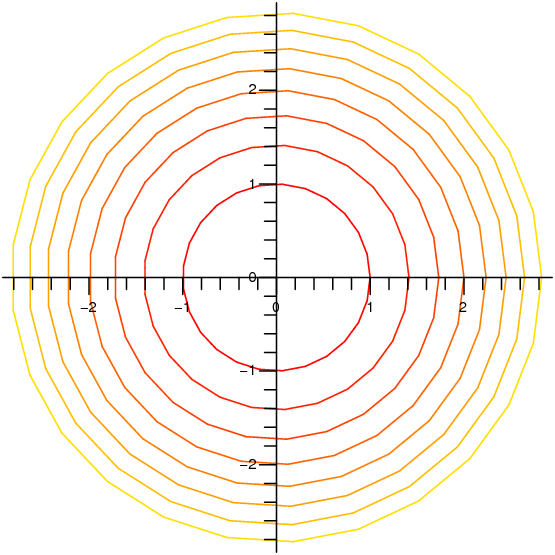
\includegraphics[width=.4\textwidth]{Figures_Part_6/parabolic_level_curves.png}
                \end{figure}
                Here, each circle represents $f(x,y)=c$ for different values of $c$.  This really \emph{is} a topographical map!
                \end{itemize}
                \end{ex}
                
                \begin{exercise}[Plane]
                Repeat this analysis for yourself for the following function:
                \[
                f(x,y)=x+y.
                \]
                \end{exercise}
                
                An important remark is that we should only use this idea to gain intuition. For one, it fails when our function is given by $f\colon \R^n \to \R$ where $n>2$.  The objects for calculus that we develop for scalar fields do not take into account the graph of the function, but just the function itself.  
                
                \subsubsection{Derivatives of scalar fields}
                        We can investigate functions of multiple variables in more ways than the single variable case.  Let us start with scalar fields.
                        
                        \begin{df}{Partial Derivatives}{partial_derivs}
                        Let $f\colon \R^3 \to \R$ be a scalar field.  Then we can consider derivatives with respect to changing each input.  For example, we define the \boldgreen{partial derivative with respect to $x$} \boldgreen{at the point $(x_0,y_0,z_0)$}, denoted $\frac{\partial f}{\partial x}(x_0,y_0,z_0)$, and put
                        \[
                        \frac{\partial f}{\partial x}(x_0,y_0,z_0)\coloneqq \lim_{\delta \to 0} \frac{f(x_0+\delta,y_0,z_0)-f(x_0,y_0,z_0)}{\delta}
                        \]
                        \end{df}
                       
                        
                        \begin{remark}
                        For partial derivatives, all but one variable are being held constant.  So, when you are computing these, be sure to treat the proper variables as constant when necessary.
                        \end{remark}
                        
                        To make notation easier to deal with, we will often just write 
                        \[
                        \frac{\partial f}{\partial x}
                        \]
                        in place of
                        \[
                        \frac{\partial f}{\partial x}(x,y,z).
                        \]
                        When we specify a point at which this partial derivative should be computed, then we must use the notation
                        \[
                         \frac{\partial f}{\partial x}(x_0,y_0,z_0),
                        \]
                        so that the meaning is unambiguous.
                        
                        \begin{exercise}
                        Define $\frac{\partial f}{\partial y}$ and $\frac{\partial f}{\partial z}$ in a similar way to the above definition.
                        \end{exercise}
                        
                        \begin{exercise}
                        Compute $\partialx$, $\partialy$, and $\partialz$ for the function 
                        \[
                        f(x,y,z)=\sin(xyz)+x+2y^2+3x^2z.
                        \]
                        \end{exercise}
                        
                        It turns out that collecting the partial derivatives as a vector is the best linear approximation to a scalar function.  We call this vector the gradient vector.
                        
                        \begin{df}{The Gradient}{gradient}
                        Given a scalar field $f(x,y,z)$, the \boldgreen{gradient of $f$ at the point $(x_0,y_0,z_0)$}, denoted $\grad f(x_0,y_0,z_0)$ is given by
                        \[
                        \grad f(x_0,y_0,z_0)=\begin{pmatrix} \partialx(x_0,y_0,z_0)\\ \partialy(x_0,y_0,z_0)\\ \partialz(x_0,y_0,z_0)\end{pmatrix}.
                        \]
                        \end{df}
                        
                        In fact, we often will consider the gradient as a vector itself.  That is, we will put
                        \[
                        \grad = \begin{pmatrix} \partialwrt{x} \\ \partialwrt{y} \\ \partialwrt{z} \end{pmatrix}.
                        \]
                        This will allow us to compute derivatives of vector fields by use of the cross and dot products.
                        
                        \begin{exercise}
                        Compute the gradient for the function
                        \[
                        f(x,y,z)=\sin(xyz)+x+2y^2+3x^2z.
                        \]
                        \end{exercise}
                        
                        \subsubsection{Properties of partial derivatives and the gradient}
                        
                        As with the one-dimensional derivative, we have some properties that will be helpful.\\
                        
                        \noindent\textbf{Partial Derivatives:}
                        \begin{enumerate}[(i)]
                            \item \textbf{Sum Rule:} Given $f(x,y,z)$ and $g(x,y,z)$, we have that
                            \[
                            \frac{\partial}{\partial x} (f(x,y,z)+g(x,y,z))=\partialx + \frac{\partial g}{\partial x}.
                            \]
                            Of course, this holds for any partial derivative.
                            \item \textbf{Constant Multiple:} Given $\lambda \in \R$ and $f(x,y,z)$, we have that
                            \[
                            \frac{\partial}{\partial x}(\lambda f(x,y,z))=\lambda \partialx.
                            \]
                            Again, this holds for any partial derivative.
                            \item \textbf{Product Rule:} Given $f(x,y,z)$ and $g(x,y,z)$ we have that
                            \[
                            \frac{\partial }{\partial x}(f(x,y,z)g(x,y,z))=\partialx g + f \frac{\partial g}{\partial x}.
                            \]
                            Ths holds for all partial derivatives.
                        \end{enumerate}
                        
                        \begin{remark}
                        The chain rule will show up eventually, but not yet.  As for the quotient rule, this also holds, but I don't show it here.
                        \end{remark}
                        
                        \noindent\textbf{The Gradient:}
                        \begin{enumerate}[(i)]
                            \item \textbf{Sum Rule:} Given $f(x,y,z)$ and $g(x,y,z)$, we have that
                            \[
                            \grad(f(x,y,z)+g(x,y,z))=\grad f(x,y,z)+\grad g(x,y,z).
                            \]
                            \item \textbf{Constant Multiple:} Given $\lambda \in \R$ and $f(x,y,z)$, we have that
                            \[
                            \grad(\lambda f(x,y,z))=\lambda \grad f(x,y,z).
                            \]
                            \item \textbf{Product Rule:} Given $f(x,y,z)$ and $g(x,y,z)$ we have that
                            \[
                            \grad(f(x,y,z)g(x,y,z))=(\grad f(x,y,z))g(x,y,z)+f(x,y,z)(\grad g(x,y,z))
                            \]
                            
                        \end{enumerate}
                        
                        We've learned how to compute partial derivatives and the gradient, but what are they really telling us? Remember that the derivative $\frac{d}{dx}$ of a function $f(x)$ tells us the rate of change of $f$ as we move in the $x$-direction.  This is very similar to what $\frac{\partial}{\partial x}$ tells us about a function $f(x,y,z)$.  So we can say the following.
                        \begin{itemize}
                            \item $\frac{\partial f}{\partial x}$ tells us how $f$ changes as we move in the $x$-direction.
                            \item $\frac{\partial f}{\partial y}$ tells us how $f$ changes as we move in the $y$-direction.
                            \item $\frac{\partial f}{\partial z}$ tells us how $f$ changes as we move in the $z$-direction.
                        \end{itemize}
                        
                        We can put these together into the gradient $\nabla f$ and know how $f$ changes in each possible direction. Let's see how the gradient acts then. 
                        
                        \begin{ex}{Gradients on the Paraboloid}{gradients_paraboloid}
                        Let us start with $f(x,y)=x^2+y^2$.  Then
                        \[
                        \nabla f(x,y) = (2x,2y).
                        \]
                        Let us plot the level curves of this surface.
                        \begin{figure}[H]
                            \centering
                            \begin{subfigure}[h]{.45\textwidth}
                            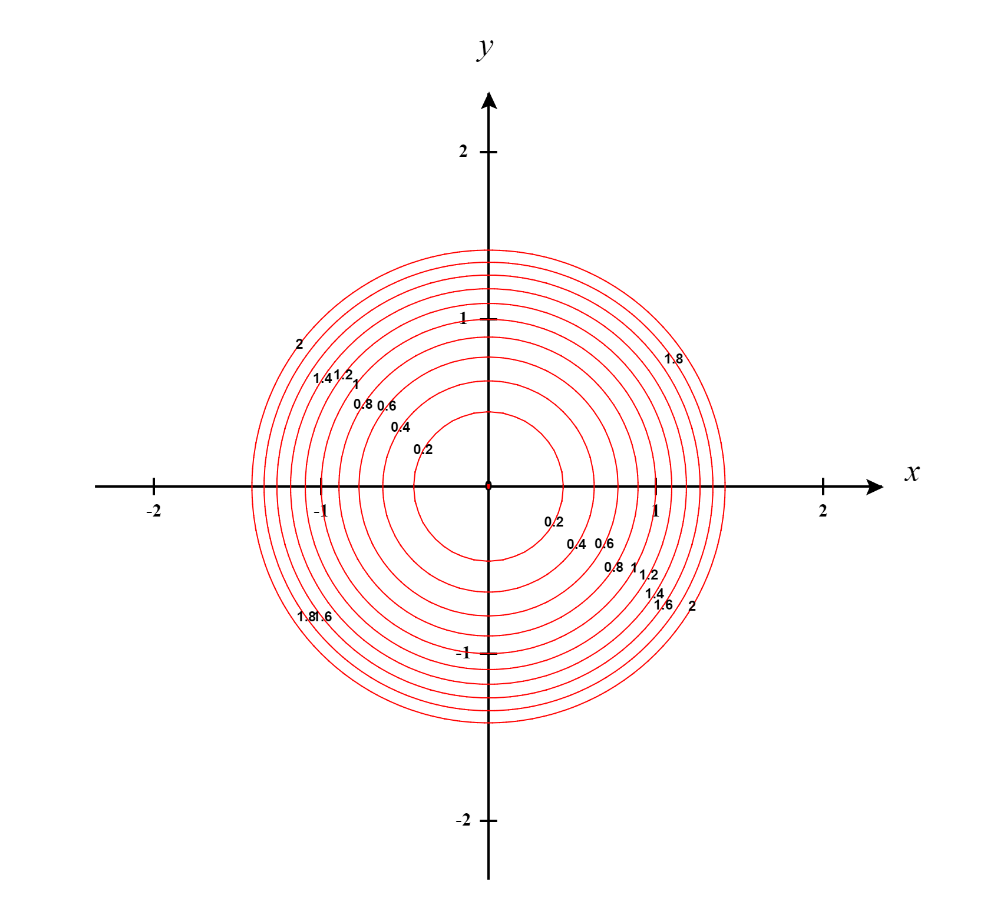
\includegraphics[width=\textwidth]{Figures_Part_6/level_curves_gradient.png}
                            \caption{Level curves of $f(x,y)$.}
                            \end{subfigure}
                            ~
                            \begin{subfigure}[h]{.45\textwidth}
                            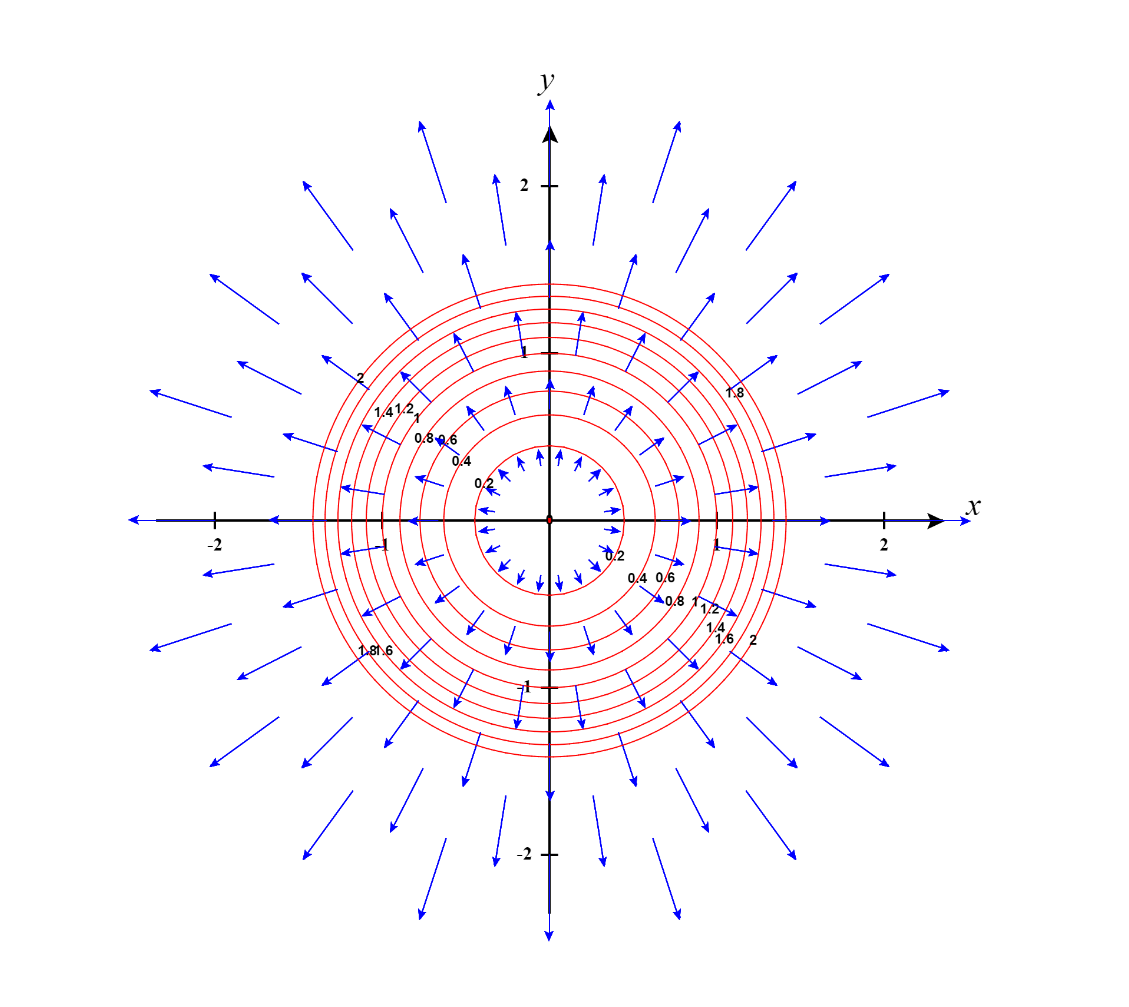
\includegraphics[width=\textwidth]{Figures_Part_6/level_curves_gradient_vectors.png}
                            \caption{Gradient vectors shown in blue.}
                            \end{subfigure}
                        \end{figure}
                        \begin{itemize}
                            \item Notice that the gradient vectors point in a direction perpendicular to the level curves and the length corresponds to how close the nearest level curve is.
                            \item The gradient is zero at the bottom of this surface.  
                        \end{itemize}
                        \end{ex}
                        
                        \begin{prop}{Gradient Points Uphill}{gradient_prop}
                        The gradient $\nabla f(x,y,z)$ is the vector that points in the direction of greatest increase for a function $f(x,y,z)$.
                        \end{prop}
                        
                        How about second partial derivatives? What can we say here. We have each of the following for a function $f(x,y)$:
                        \begin{itemize}
                            \item $\frac{\partial^2 f}{\partial x^2}$
                            \item $\frac{\partial^2 f}{\partial y^2}$
                            \item $\frac{\partial}{\partial y}\frac{\partial f}{\partial x}$
                            \item $\frac{\partial}{\partial x}\frac{\partial f}{\partial y}$
                        \end{itemize}
                        
                        Recall what $\frac{d^2 f}{dx^2}$ meant for a function $f(x)$.  This told us how $f$ was curving (or what concavity $f$ had). The story is similar for these partial derivatives.
                        
                        \begin{itemize}
                            \item $\frac{\partial^2 f}{\partial x^2}$ tells us about the concavity (or curvature) of $f$ as we move in the $x$ direction.
                            \item $\frac{\partial^2 f}{\partial y^2}$ tells us about the concavity (or curvature) of $f$ as we move in the $y$ direction.
                            \item We actually have that $\frac{\partial}{\partial y}\frac{\partial f}{\partial x}=\frac{\partial}{\partial x}\frac{\partial f}{\partial y}$.  This interpretation is a bit hard to deal with.  Let's not worry too much about it.
                        \end{itemize}
                        
                        \begin{prop}{Partial Derivatives Commute}{partials_commute}
                        We have that
                        \[
                        \frac{\partial}{\partial y}\frac{\partial f}{\partial x}=\frac{\partial}{\partial x}\frac{\partial f}{\partial y}.
                        \]
                        Moreover, for functions of more variables, we can say that the order we take derivatives does not matter.
                        \end{prop}
                        
                        \begin{exercise}
                        Given $f(x,y)=x^2+y^2$, compute
                        \[
                        \frac{\partial^2 f}{\partial x^2}, ~ \frac{\partial^2 f}{\partial y^2}, ~ \frac{\partial}{\partial y}\frac{\partial f}{\partial x},~ \frac{\partial}{\partial x}\frac{\partial f}{\partial y}.
                        \]
                        What can we say about the curvature of $f$ in the two directions? Does this make sense?
                        \end{exercise}
                        
                        \subsection{Directional Derivatives}
                        
                        Related to the notion of partial differentiation and the gradient is that of finding the derivative of a function in a given direction.  Say that we are given a scalar field $f(x,y,z)$, and we are also given a unit vector $\unitvec$.  Then, we can compute the \boldgreen{directional derivative of $f$ in the direction $\unitvec$} by
                        \[
                        \frac{\partial f}{\partial \unitvec} = \unitvec \cdot \grad f.
                        \]
                        There is another way to define this derivative, but it requires a bit more work to derive.
                        
                                               
                        One can see that we can recover partial derivatives via this notion as well.  For example, if we let $\unitvec = \xhat$, then we have
                        \[
                        \frac{\partial f}{\partial \unitvec} = \xhat \cdot \grad f = \partialx.
                        \]
                        We can think of directional derivatives as generalizations of partial derivatives where we allow for computing the derivative of our function $f$ in a direction other than the ones given by the chosen basis.
                        
                        \section{Optimization}
                        In single variable calculus, we optimized functions $f(x)$ by finding the point $x_0$ where 
                        \[
                        f'(x_0)=0.
                        \]
                        We called this a \emph{critical point}. We found if this optimizer $x_0$ was a maximizer or minimizer by checking the sign of second derivative $f''(x_0)$. We had
                        \begin{align*}
                            \textrm{Maximum: }& f''(x_0)<0\\
                            \textrm{Minimum: }& f''(x_0)>0.
                        \end{align*}
                        
                        In higher dimensions, this idea works similarly. We just have more to check. 
                        
                        \begin{df}{Stationary Points}{stationary_points}
                        Given a function $f(x,y)$, we call a point $(x_0,y_0)$ a \textbf{stationary point} if 
                        \[
                        \nabla f(x_0,y_0) = \mathbf{0}.
                        \]
                        \end{df}
                        
                        As before, we will use second derivatives to find out whether this is a maximum or a minimum.
                        
                        \begin{prop}{Maximizers and Minimizers}{max_min}
                        A stationary point $(x_0,y_0)$ is a 
                        \begin{align*}
                            \textrm{Maximizer if~ }& \frac{\partial^2 f}{\partial x^2} <0 \textrm{ ~and~ } \frac{\partial^2 f}{\partial y^2}<0,\\
                            \textrm{Minimizer if~ }& \frac{\partial^2 f}{\partial x^2} >0 \textrm{ ~and~ } \frac{\partial^2 f}{\partial y^2}>0,\\
                            \textrm{Saddle if otherwise.}
                        \end{align*}
                        \end{prop}
                        
                        \begin{exercise}
                        Let
                        \[
                        f(x,y) = \frac{xy}{e^{x^2+y^2}}.
                        \]
                        \begin{enumerate}[(a)]
                            \item Find all stationary points for $f$.
                            \item Determine whether these points are minimizers or maximizers.
                        \end{enumerate}
                        \end{exercise}
                        
                        \begin{exercise}
                        Show that $f(x,y)=xy$ has a saddle point at $(0,0)$.
                        \end{exercise}
                        
                        Some optimization problems cannot be solved just using this technique.  If you are interested, consider reading about \boldgreen{Lagrange multipliers}.
                        
%                        \subsubsection{Lagrange Multipliers}
%                        Often times we are given a situation that we wish to find an optimum solution to, but we are somehow constrained.  A biological example would be fixing a given volume for a red blood cell, and finding the optimum shape so that oxygen diffusion is maximized.  A physical example would be finding the fastest path between two points when moving through a medium with varying viscosity.
%                        
%                        The idea is relatively tame. We are given the function to optimize
%                        \[
%                        f(x,y,z)
%                        \]
%                        and the constraining function
%                        \[
%                        g(x,y,z)=k.
%                        \]
%                        Then we must solve the equation
%                        \[
%                        \nabla f(x,y,z) = \lambda \nabla g (x,y,z)
%                        \]
%                        where $\lambda$ is called the \textbf{Lagrange multiplier}. Let's work through an example of solving this.
%                        
%                        \begin{ex}{Largest Box}{largest_box}
%                        Let's find the dimensions of the box with the largest volume if the total surface area is $64 cm^2$.  We must determine our function to optimize, which is the volume function
%                        \[
%                        V(x,y,z) = xyz.
%                        \]
%                        Our constraint is the surface area function $A(x,y,z)$ must be
%                        \[
%                        g(x,y,z)=2xy+2xz+2yz=64,
%                        \]
%                        which we will simplify as
%                        \[
%                        xy+xz+yz = 32.
%                        \]
%                        \begin{enumerate}
%                            \item We first take
%                            \[
%                            \nabla f(x,y,z) = \begin{bmatrix} yz \\ xz \\ xy \end{bmatrix}
%                            \]
%                            and
%                            \[
%                            \nabla g(x,y,z) = \begin{bmatrix} 2y+2z \\ 2x+2z \\ 2x+2y\end{bmatrix}.
%                            \]
%                            \item This gives us four equations to solve. Three are from the equation $\nabla f(x,y,z) =\nabla g(x,y,z)$
%                            \begin{align}
%                                yz &= \lambda (y+z)\\
%                                xz &= \lambda (x+z)\\
%                                xy &= \lambda (x+y),
%                            \end{align}
%                            and one is from the constraint $g(x,y,z)=64$
%                            \[
%                            xy+xz+yz = 32.
%                            \]
%                            \item Working through solving these can be nontrivial.  In this case, we can do the following: Multiply (1) by $x$, (2) by $y$, and $(3)$ by $z$.  Which gives us
%                            \begin{align*}
%                                xyz &= \lambda x(y+z)\\
%                                xyz &= \lambda y(x+z)\\
%                                xyz &= \lambda z(x+y)
%                            \end{align*}
%                            Now we can set the first two equal to find
%                            \[
%                            \lambda x(y+z)=\lambda y(x+z)
%                            \]
%                            which simplifies to 
%                            \[
%                            \lambda (xz-yz)=0
%                            \]
%                            meaning that $\lambda =0$ or $xz=yz$. Note that $\lambda =0$ is not possible since that will end up giving us zero surface area and we won't satisfy the constraint.
%                            
%                            Now $xz-yz=0$ means that $x=y$, which we can substitute back into the equations later. 
%                            
%                            We can set the last two equal to find
%                            \[
%                            \lambda y (x+z)=\lambda z(x+y)
%                            \]
%                            which with similar work tells us $z=y$.  So now we make note of $x=y$ and we have $x=y=z$.  
%                            
%                            So now we use the constraint equation with $x=y=z$ and find that we have
%                            \[
%                            x^2+y^2+z^2 = 3x^2 = 32
%                            \]
%                            which means that $x\approx 3.266$.  Thus
%                            \[
%                            V(3.266,3.266,3.266)\approx 34.8376
%                            \]
%                            is the largest volume.  \emph{This means our ideal solution is a cube!} 
%                            
%                        \end{enumerate}
%                        \end{ex}
                        
                       
                
                
                \section{Integrals of Scalar Fields}
                
                In one dimension, we integrated functions in order to sum up values over a given interval.  Geometrically, this gave us the net area under a curve.  In this case, we took a function $f(x)$ and an interval $[a,b]$ and we wrote
                \[
                \int_a^b f(x) dx.
                \]
                When we work in higher dimensions, we have to be a bit more careful.  Let us instead rephrase this problem by instead specifying a region $\Omega = [a,b]$ and a function $f$, then we would put
                \[
                \int_\Omega f d\Omega = \int_a^b f(x)dx.
                \]
                The difference we wish to establish is that the integral we are performing depends on the coordinates in which we choose.  Later on, this will become very apparent when we consider new forms of coordinate systems (e.g., polar coordinates).  
                
                What we put above is simply a change of notation that allows for greater versatility.  Imagine we have a region in the plane $\Omega$ and a scalar field $f\colon \Omega \to \R$, then we can plot the graph of that function in Cartesian coordinates by thinking of the function $f$ as taking in an $(x,y)$ pair, and placing $f(x,y)$ as the height above the $xy$-plane.
                \begin{figure}[H]
                	\centering
                	\def\svgwidth{0.75\columnwidth}
                	\input{Figures_Part_6/surface_graph.pdf_tex}
                \end{figure}
                A region $\Omega$ is given in the plane with respect to some coordinates.  For example, we may specify the region in the plane by $x_0 \leq x \leq x_1$ and $y_0 \leq y \leq y_1$, and so we write our function with respect to these choices.  Then, say we want to compute the volume under the surface given by the graph $(x,y,f(x,y))$, we would then compute
                \[
                \int_{y_0}^{y_1} \int_{x_0}^{x_1} f(x,y)dxdy.
                \]
                This is known as a \boldgreen{double integral}.  But, we can phrase this double integral without reference to any coordinate choice by taking
                \[
                \iint_\Omega f d\Omega.
                \]
             	We sill stick with this notation as we continue onward.
             	
             	Nothing changes as we increase the dimension; just the number of integrals we must compute will increase.  Below, we will compute examples in varying dimensions.
             	
             	
             	        
             	        \subsubsection{One Dimensional Case}
             	        Briefly, let us compute an example in one dimension so that we can see how this analogy generalizes.
             	        
             	        \begin{ex}{One-Dimensional Integral}
             	        Let $f(x) = x^2+2$, $a=1,$ and $b=2$. Then we want to find
             	        \[
             	        \int_a^b f(x)dx = \int_1^2 x^2+2dx.
             	        \]
             	        Then we use the \emph{Fundamental Theorem of Calculus}. So, we find the antiderivative of the integrand and evaluate at the endpoints as follows
             	        \begin{align*}
             	            \int_1^2 x^2+2dx &= \left[ \frac{x^3}{3}+2x\right]_1^2\\
             	            &= \left(\frac{2^3}{3}+2(2)\right) - \left( \frac{1^3}{3}+2(1)\right)\\
             	            &= \frac{13}{3}.
             	        \end{align*}
             	        \end{ex}
             	        
             	        \subsubsection{Two Dimensional Case}
             	        
             	        Say we are now given a function $f(x,y)$ and bounds on both the $x$ and $y$ by
             	        $x_0 \leq x \leq x_1$ and $y_0 \leq y \leq y_1$.  We then wish to evaluate
             	        \[
             	        \int_{y_0}^{y_1} \int_{x_0}^{x_1} f(x,y)dxdy.
             	        \]
             	        You can think of this integral as being the \emph{net} volume under the surface given by $f(x,y)$.  
             	        
             	        How do we compute such an integral? The answer is iteratively.  Let's see how we do this with a concrete example.
             	        
             	        \begin{ex}{Two-Dimensional Integral}{2d_int}
             	        Let $f(x,y)=xy$, $x_0=1$, $x_1=2$, $y_0=3$ and $y_1=4$.  So, we want to evaluate
             	        \[
             	        \int_{y_0}^{y_1}\int_{x_0}^{x_1} f(x,y)dxdy = \int_3^4 \int_1^2 xy dxdy.
             	        \]
             	        The way we do this is by first evaluating the integral with respect to $x$ (holding $y$ constant) and then integrate with respect to $y$ ($x$ will not appear here). So, we integrate from the inside out.  
             	        
             	        Let's start by integrating with respect to $x$. We take
             	        \begin{align*}
             	            \int_1^2 xy dx &= \left[ \frac{x^2y}{2}\right]_1^2\\
             	            &= \left( y\frac{2^2}{2}\right) - \left(y\frac{1^2}{2}\right)\\
             	            &=\frac{3}{2}y.
             	        \end{align*}
             	        Now we take this function of $y$, and we integrate this with the bounds we are given.  
             	        \begin{align*}
             	            \int_3^4 \frac{3}{2}y dy &= \left[ \frac{3y^2}{4} \right]_3^4\\
             	            &= \frac{21}{4}.
             	        \end{align*}
             	        So we say that
             	        \[
             	        \int_3^4 \int_1^2 xy dxdy = \frac{21}{4}.
             	        \]
             	        
             	        Let's walk through the steps again. We did
             	        \begin{align*}
             	            \int_{y_0}^{y_1} \int_{x_0}^{x_1} f(x,y)dxdy&= \int_3^4\int_1^2 xy dxdy\\
             	            &= \int_3^4 \frac{3}{2}ydy \\
             	            &= \frac{21}{4}.
             	        \end{align*}
             	        \end{ex}
             	        
             	        \subsubsection{Three Dimensional Case}
             	        
             	        Integration here is performed in the same way.  We are given a function $f(x,y,z)$ and bounds on $x$, $y$, and $z$ such as $x_0\leq x \leq x_1$, $y_0\leq y\leq y_1$, and $z_0\leq z \leq z_1$. Then we evaluate
             	        \[
             	        \int_{z_0}^{z_1}\int_{y_0}^{y_1}\int_{x_0}^{x_1} f(x,y,z)dxdydz.
             	        \]
             	        Let's work through an example.
             	        
             	        \begin{ex}{Three-Dimensional Integral}{3d_int}
             	        Let
             	        \[
             	        f(x,y,z)=2x + 8xyz + 3,
             	        \]
             	        and say we want to integrate over the rectangular prism given by $x_0 = 0$, $x_1=1$, $y_0=2$, $y_1=3$, $z_0 =4$, $z_1=5$.  Then we want to find
             	        \[
             	        \int_{z_0}^{z_1}\int_{y_0}^{y_1}\int_{x_0}^{x_1} f(x,y,z)dxdydz = \int_4^5 \int_2^3 \int_0^1 2x+8xyz+3dxdydz.
             	        \]
             	        We do this iteratively.  So we first evaluate the $x$ integral holding the other variables constant for now.
             	        \begin{align*}
             	            \int_0^1 2x+8xyz+3 dx &= \left[ x^2 + 4x^2yz+3x\right]_0^1\\
             	            &= \left( 1^2 + 4(1)^2yz+3(1)\right) - \left( 0^2+4(0)^2yz+3(0)\right)\\
             	            &= 4yz+4.
             	        \end{align*}
             	        We then take this, and integrate with respect to $y$.
             	        \begin{align*}
             	            \int_2^3 4yz + 4 dy &= \left[ 2y^2z+4y\right]_2^3\\
             	            &= (4(3)^2z+4(3))-(4(2)^2z+4(2))\\
             	            &= 10z+4.
             	        \end{align*}
             	        Lastly, we integrate with respect to $z$
             	        \begin{align*}
             	            \int_4^5 10z+4 dz &= \left[ 5z^2+4z\right]_4^5\\
             	            &= (5(5)^2+4(5))-(5(4)^2+4(4))\\
             	            &=49.
             	        \end{align*}
             	        So we say that
             	        \[
             	        \int_4^5 \int_2^3 \int_0^1 2x+8xyz+3dxdydz = 49.
             	        \]
             	        Again, let's walk through the steps a bit
             	        \begin{align*}
             	            \int_{z_0}^{z_1}\int_{y_0}^{y_1}\int_{x_0}^{x_1} f(x,y,z)dxdydz &= \int_4^5 \int_2^3 \int_0^1 2x+8xyz+3dxdydz\\
             	            &= \int_4^5 \int_3^4 4yz+4dydz\\
             	            &= \int_4^5 10z+4dz\\
             	            &= 49.
             	        \end{align*}
             	        \end{ex}
             	       
             	       \begin{remark}
             	       There is nothing stopping us from integrating, say, a 3-dimensional scalar field over a 2-dimensional domain $\Omega$. The definitions above work in this situation.  
             	       \end{remark}
             	       
             	       \begin{ex}{Integrating a Scalar Fields on Subsurfaces}{integrating_subsurfaces}
                			Consider the same scalar field $f(x,y,z) = 2x + 8xyz + 3$, but instead integrated over the rectangle $\Omega$ defined by $0\leq x,y \leq 1$ and $z=1$.  Then, we have
                			\begin{align*}
                				\iint_\Omega f(x,y,z)d\Omega &= \int_0^1 \int_0^1 f(x,y,1)dxdy\\
                				&= \int_0^1 \left(x^2 + 4x^2y+3x\right)\vert_0^1 dy\\
                				&= \int_0^1 1+4y+3 dy\\
                				&= \left(2y^2 + 4y\right)\vert_0^1\\
                				&= 6.
                			\end{align*}
                		\end{ex}
                
                \subsection{Line Integrals}
                       For the purpose of visualization, we will look at scalar fields of two variables and curves in the plane.  Our set up will have $f(x,y)$ and $\gamma(t)$ over the time $t=a$ to $t=b$.
                       
                       We want to understand the following:
                       \[
                       \int_{\curvegamma} fd\curvegamma \coloneqq \int_a^b f(\curvegamma(t))\left|\tangentgamma(t)\right|dt.
                       \]
                       Intuitively speaking, this integral finds the area under the curve $\curvegamma$ along the graph of $f$.  This is analogous to what we did in one dimension! See the following figure.
                       \begin{figure}[H]
                           \centering
                           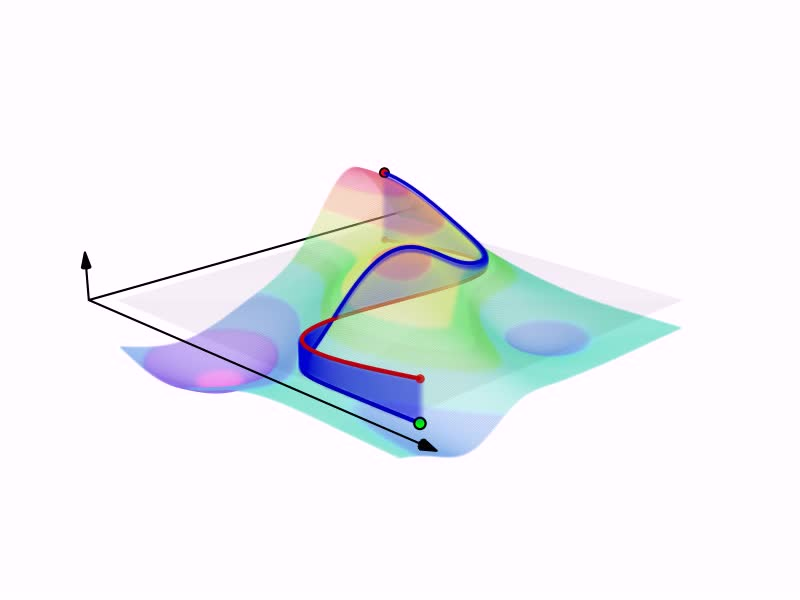
\includegraphics[width=.5\textwidth]{Figures_Part_6/Line_integral_of_scalar_field.jpg}
                       \end{figure}
                       
                       \begin{ex}{Length of a curve}{length_of_curve}
                       Let $f(x,y,z)=1$ and $\curvegamma(t)$ be a curve over $t=a$ to $t=b$.  Then the line integral
                       \[
                       \int_{\curvegamma} fd\curvegamma = \int_a^b \left|\tangentgamma(t)\right|dt
                       \]
                      which is the length of the curve $\curvegamma$.
                       \end{ex}
                       
                       \begin{ex}{Line Integral on a Paraboloid}{line_int_parabooid}
                       Consider the function $f(x,y)=x^2+y^2$ and $\curvegamma(t)=\begin{pmatrix} t \\ t \end{pmatrix}$ over $t=0$ to $t=1$.  Then the line integral
                       \[
                       \int_{\curvegamma} fd\curvegamma = \int_0^1 f(\curvegamma(t))\left|\tangentgamma(t)\right|dt.
                       \]
                       We have
                       \begin{itemize}
                           \item $f(\curvegamma(t))=t^2+t^2=2t^2.$
                           \item $\left|\tangentgamma(t)\right|=\left|\begin{pmatrix} 1 \\ 1\end{pmatrix}\right|=\sqrt{2}.$
                       \end{itemize}
                       So we have
                       \[
                       \int_{\curvegamma} fd\curvegamma = \int_0^1 2\sqrt{2}t^2dt.
                       \]
                       This evaluates to $\frac{2\sqrt{2}}{3}$.
                       \end{ex}
                       
                       \begin{exercise}
                       Integrate $f(x,y)=x+y$ along the curve $\curvegamma(t)=\begin{pmatrix} t \\ 0 \end{pmatrix}$ from $t=0$ to $t=1$. What do you notice about this? Can we tie this to one-dimensional integration?
                       \end{exercise}
                       
                      
                       
        
        


%
%\chapter{Differential and Integration Operators}
%\input{Chapters_Part_6/differential_operators.tex}
%
%\chapter{Coordinate Systems and Parameterization}
%\section{Level surfaces}
                In the planar case, we would often have to specify a set of points like
                \[
                x^2+y^2=1
                \]
                which is the circle.  
                
                In higher dimensions, we can do the same in order to visualize functions of the form $f\colon \R^3\to \R$ written as $f(x,y,z)$.  If we pick some constant $c$ and write
                \[
                f(x,y,z)=c
                \]
                then we will get the \textbf{level surfaces} for the function $f(x,y,z)$.  Visualizing functions of three variables (or more) $f(x,y,z)$ requires us to visualize in four or more dimensions. So we often reduce the problem to visualizing level surfaces.
                
                \begin{ex}{A Sphere as a Level Surface}{sphere_lev_surf}
                We can consider the following function
                \[
                f(x,y,z)=x^2+y^2+z^2.
                \]
                If we take the one level set, that is the points $(x,y,z)$ that satisfy
                \[
                x^2+y^2+z^2=1
                \]
                then we get the \emph{2-sphere}.  These are the set of points that are all a distance one from the origin.  Here is a picture:
                \begin{figure}[H]
                    \centering
                    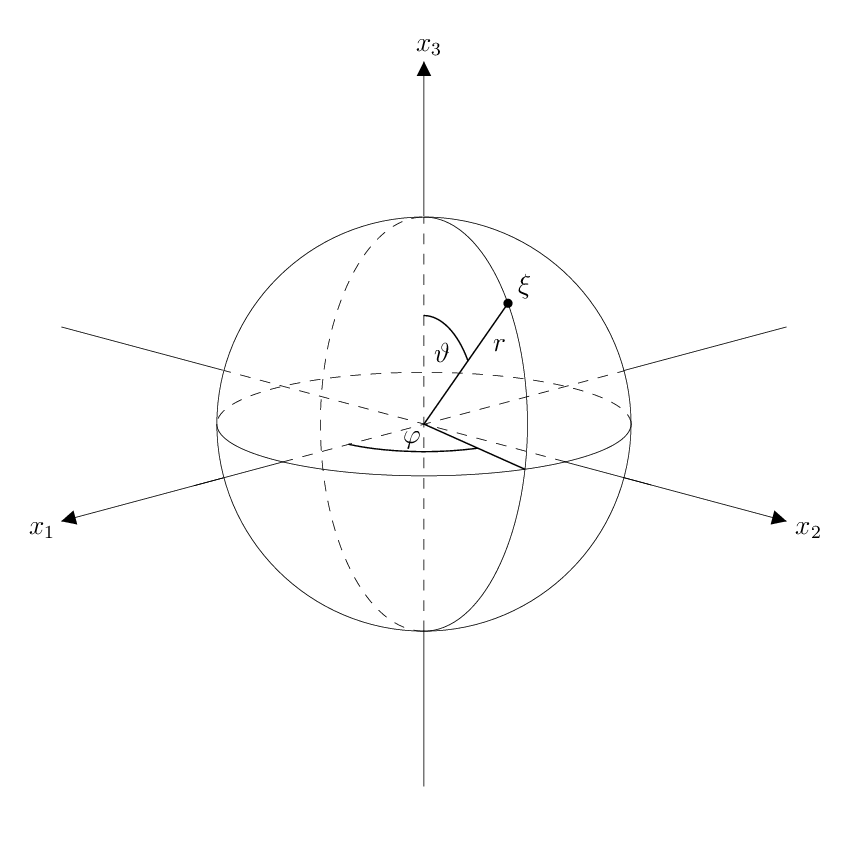
\includegraphics[width=.4\textwidth]{Figures_Part_6/sphere.png}
                \end{figure}
                \end{ex}
                
                \begin{ex}{The Hyperboloids}{hyperboloids}
                Consider a family of surfaces given by the level surfaces of
                \[
                f(x,y,z)=x^2+y^2-z^2.
                \]
                \begin{itemize}
                    \item If we take $c=0$ and set
                    \[
                    x^2+y^2-z^2=0.
                    \]
                    then we find the 0 level surface. In this case, we can do a bit of work to find
                    \[
                    z=\pm \sqrt{x^2+y^2}.
                    \]
                    Notice, if we pick any value for $z$, that we get a circle at that level!  When $z=0$, we get a single point.  It turns out that we get the \emph{(double) cone} surface which looks like
                    \begin{figure}[H]
                        \centering
                     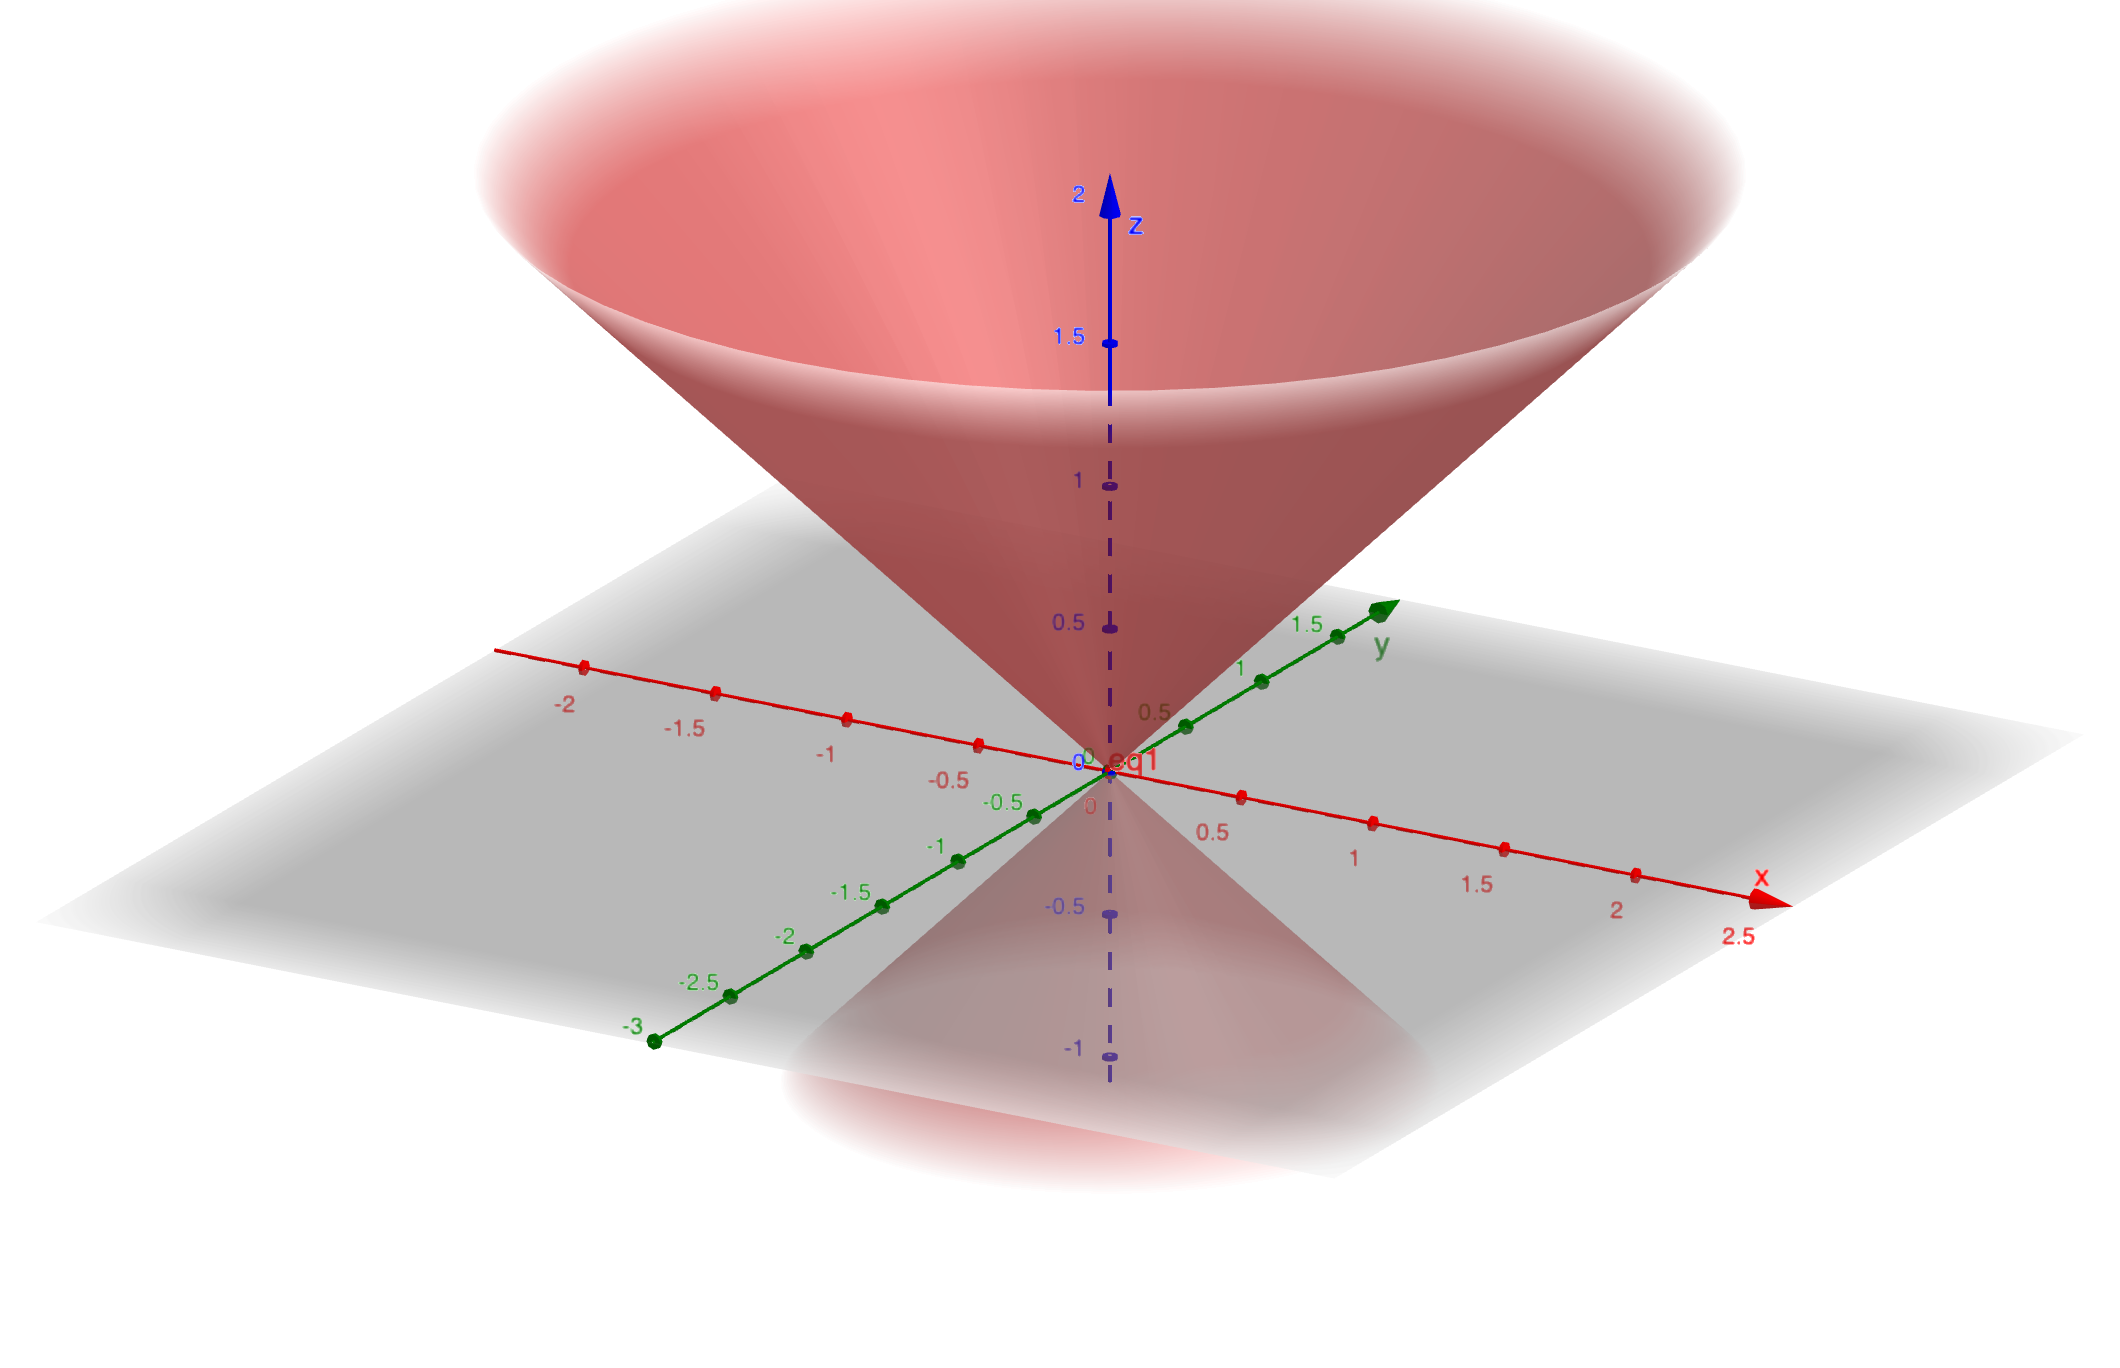
\includegraphics[width=.4\textwidth]{Figures_Part_6/cone_surface.png}
                    \end{figure}
                    
                    \item If we take $c=1$ and set
                    \[
                    x^2+y^2-z^2=1
                    \]
                    we get the \emph{hyperboloid of one sheet}.  This looks like
                    \begin{figure}[H]
                        \centering
                        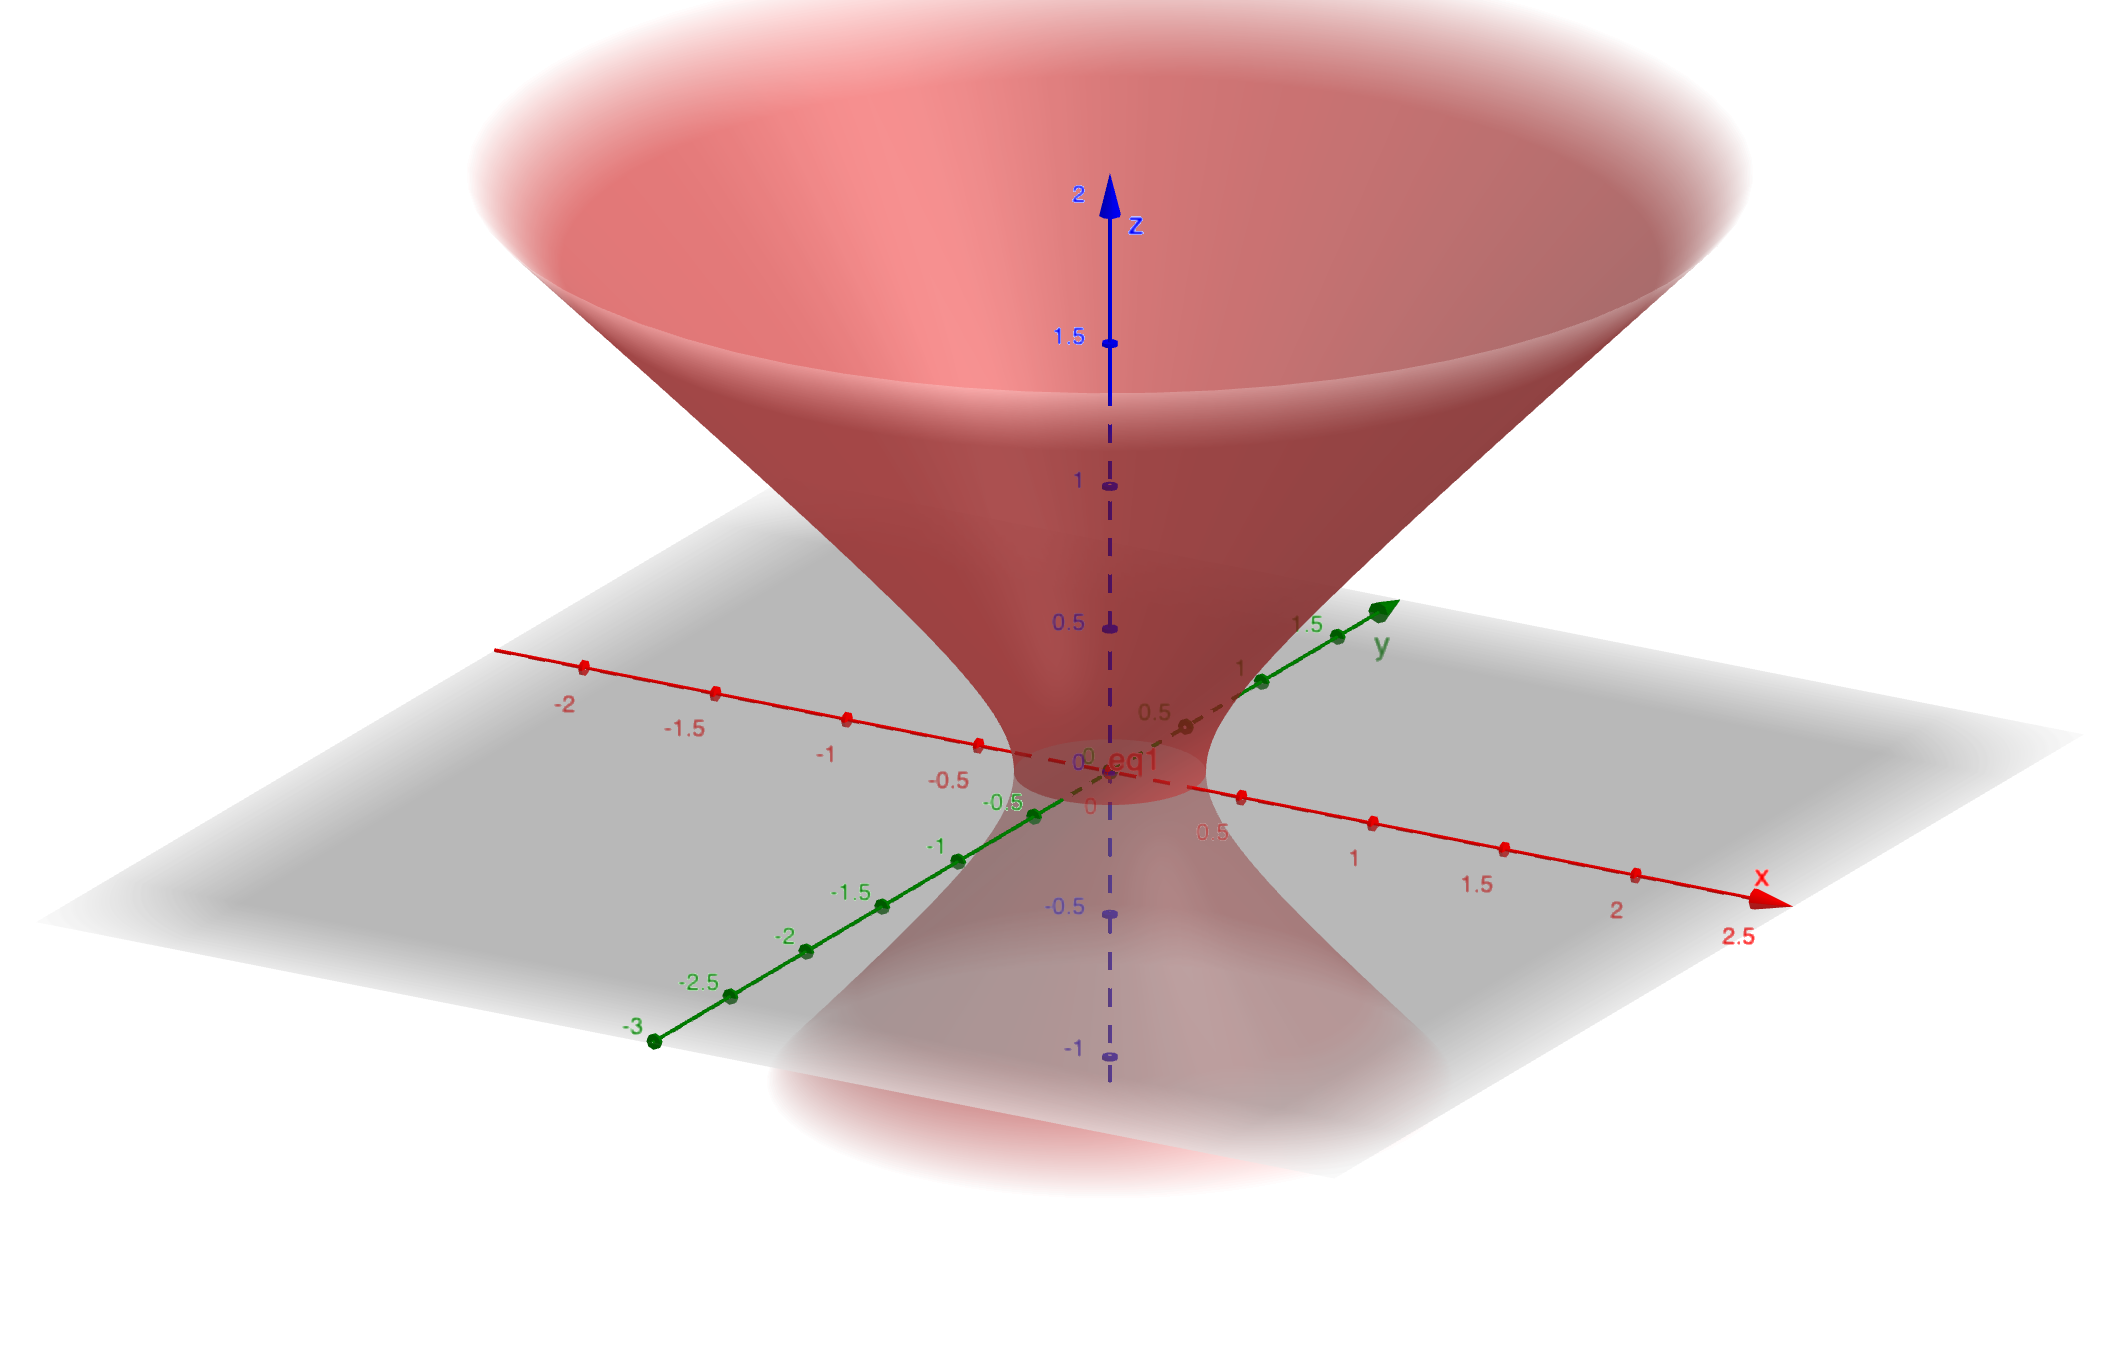
\includegraphics[width=.4\textwidth]{Figures_Part_6/hyperboloid_1_sheet.png}
                    \end{figure}
                    
                    \item If we take $c=-1$ and set
                    \[
                    x^2+y^2-z^2=-1
                    \]
                    we get the \emph{hyperboloid of two sheets}.  This looks like
                    \begin{figure}[H]
                        \centering
                        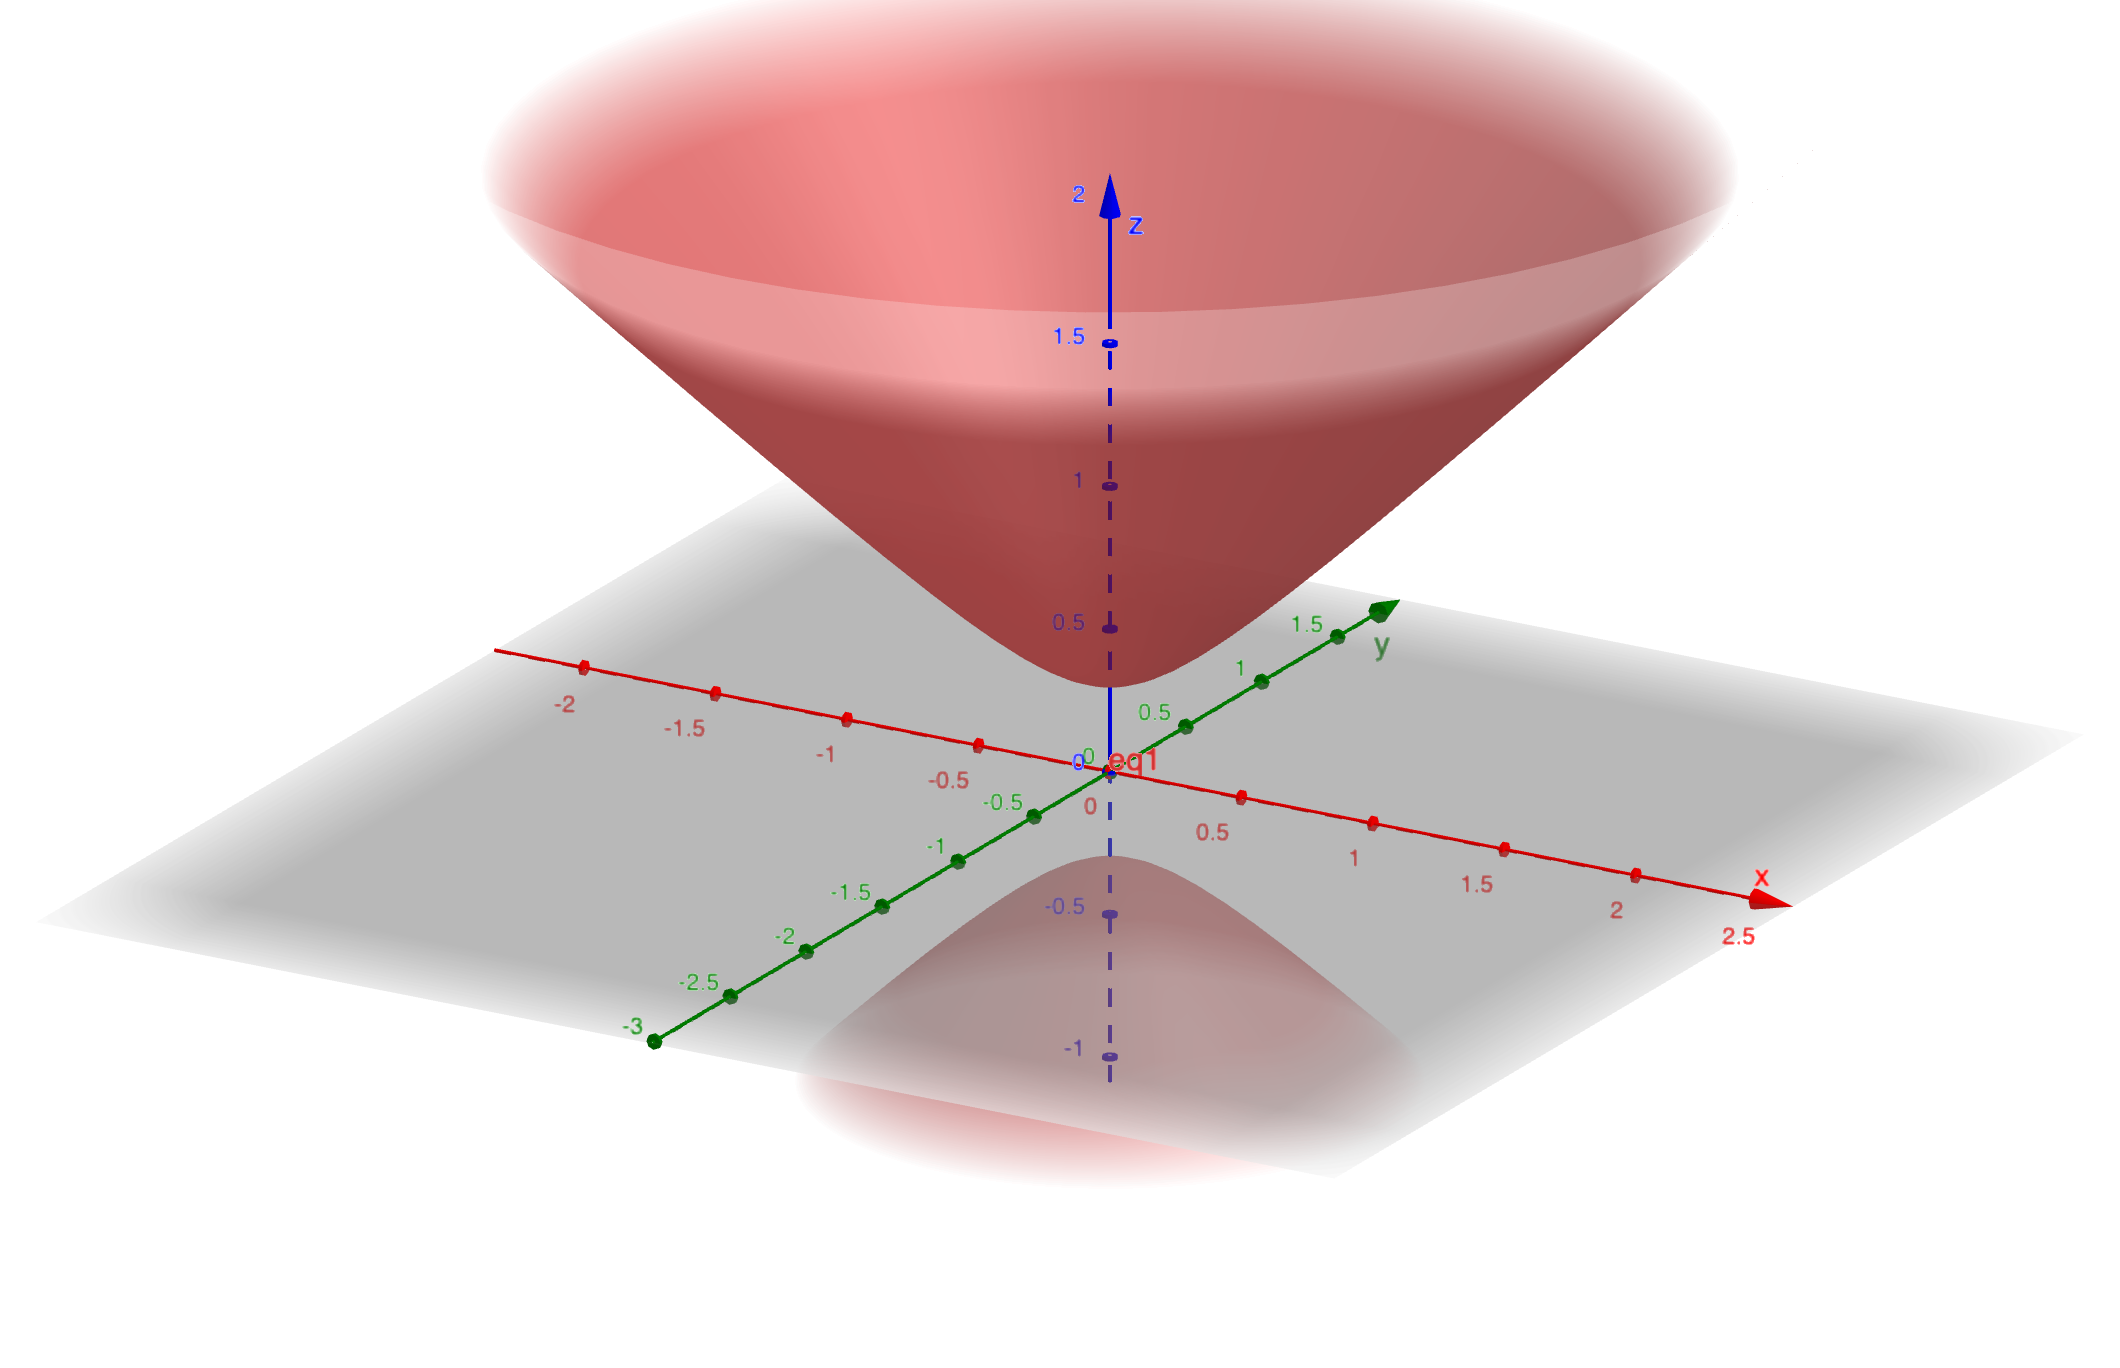
\includegraphics[width=.4\textwidth]{Figures_Part_6/hyperboloid_2_sheet.png}
                    \end{figure}
                \end{itemize}
                \end{ex}
                
                \begin{ex}{The Torus}{torus}
                For this example, I will choose specific nice numbers, but this is a yet another case of a level surface.  Take
                \[
                \left(5-\sqrt{x^2+y^2}\right)^2+z^2=2.
                \]
                This gives us the \emph{torus} with inner radius (the radius from the center of the donut hole to the center of the tube) $5=R$ and tube radius $2=r$. This looks like
                \begin{figure}[H]
                    \centering
                    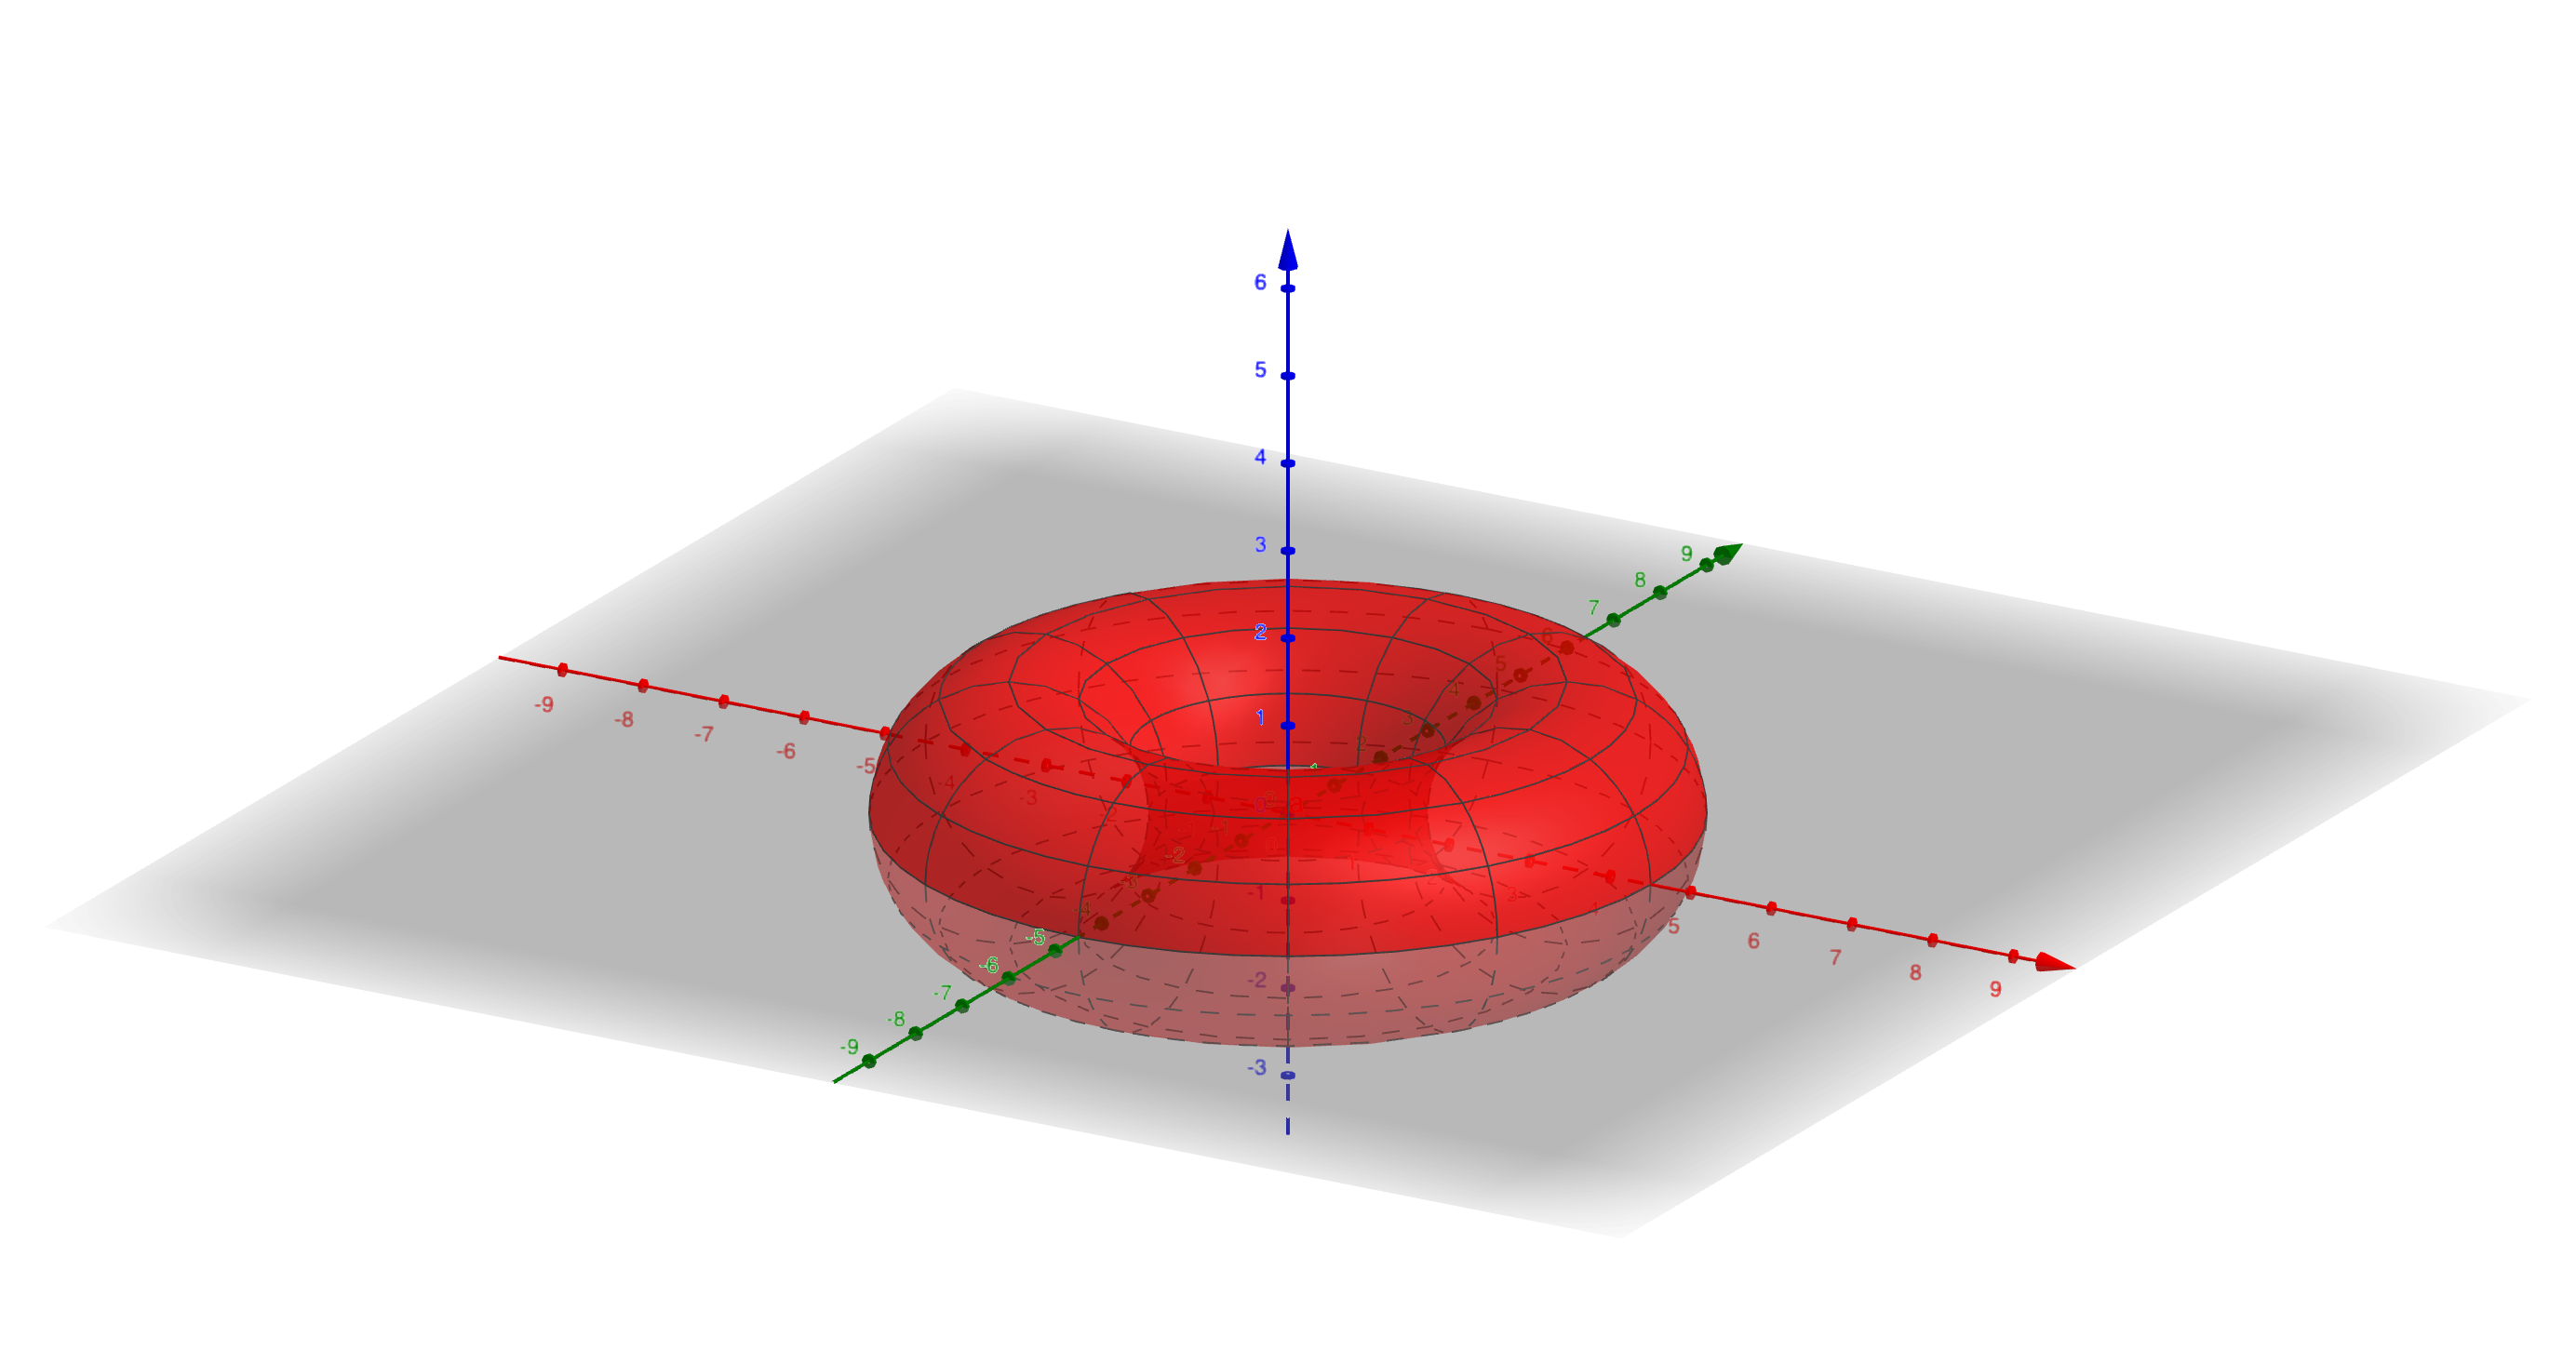
\includegraphics[width=.4\textwidth]{Figures_Part_6/torus.png}
                \end{figure}
                \end{ex}
                
                
                We have given ourselves ways of understanding the scalar functions and curves, but still need to develop a manner to understand vector fields.  We will not only need to understand vector fields in their own right, but we will need them in order to investigate how the scalar fields change from point to point.  Roughly speaking, the ``derivative" of a scalar field will be a vector field.
                
                 \section{Approximation and the Tangent Space}
                                        Sometimes it is helpful to know what a surface looks like up close.  In this case, the surface is best approximated by a plane.  This is analogous to how you can approximate functions of a single variable by a line.
                                        
                                        \begin{exercise}
                                        Compute the tangent line to $f(x)=2x^2+5$ at the point $x_0=3$.
                                        \end{exercise}
                                        
                                        \subsubsection{Equation for a Plane}
                                        
                                        We haven't worked much with planes in space yet, but we have seen surfaces.  In some sense, planes are the easiest surfaces.  They are, after all, linear objects.
                                        
                                        \begin{ex}{Plane and Normal}{plane_normal}
                                        The equation for a plane is given by
                                        \[
                                        ax+by+cz+ d = 0.
                                        \]
                                        Notice that this is a linear equation.
                                        
                                        Then the \emph{normal vector} to the plane is given by 
                                        \[
                                        \mathbf{n} = \begin{bmatrix} a \\ b \\ c\end{bmatrix}.
                                        \]
                                        We can see a diagram of this here.
                                        \begin{figure}[H]
                                            \centering
                                            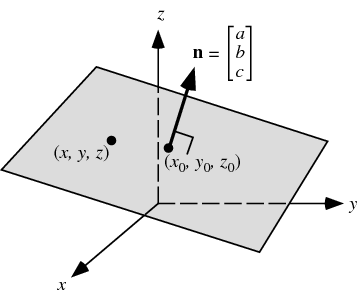
\includegraphics[width=.4\textwidth]{Figures_Part_6/plane_n.png}
                                        \end{figure}
                                        \end{ex}
                                        
                                        Now, if we are given a surface (defined as a level surface or as the graph of a function), we can compute an approximation at a point called the \emph{tangent plane}.
                                        
                                        \begin{ex}{Tangent Plane to Paraboloid}
                                        Consider the function 
                                        \[
                                        f(x,y)=-x^2-y^2.
                                        \]
                                        Then the graph of the function is given by plotting the points
                                        \[
                                        (x,y,f(x,y)).
                                        \]
                                        We compute the tangent plane by computing partial derivatives. We take
                                        \begin{align*}
                                        \frac{\partial f}{\partial x} &= -2x\\    
                                        \frac{\partial f}{\partial y} &= -2y.
                                        \end{align*}
                                        Then the equation for a tangent plane at the point $(x_0,y_0,f(x_0,y_0))$ is given by
                                        \[
                                        z-f(x_0,y_0)=\partialx (x-x_0)+\partialy (y-y_0).
                                        \]
                                        So in our case, we have
                                        \[
                                        z-(-x_0^2-y_0^2)=-2x_0(x-x_0)-2y_0(y-y_0).
                                        \]
                                        Pictorially, it looks as follows (letting $p=(x_0,y_0,f(x_0,y_0))$):
                                        \begin{figure}[H]
                                            \centering
                                            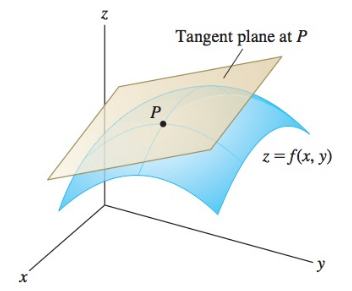
\includegraphics[width=.4\textwidth]{Figures_Part_6/tangent-planes-1.png}
                                        \end{figure}
                                                
                                        \end{ex}
                                        
                                        \begin{ex}{Tangent Vectors}{tangent_vectors}
                                        Another way to understand this is to compute the \emph{tangent vectors} at a point. Take the same function $f(x,y)=-x^2-y^2$ and compute
                                        \begin{align*}
                                            \frac{\partial}{\partial x}\begin{bmatrix} x \\ y \\ f(x,y)\end{bmatrix} &= \begin{bmatrix} 1\\ 0 \\ -2x\end{bmatrix}\\
                                            \frac{\partial}{\partial y}\begin{bmatrix} x \\ y \\ f(x,y)\end{bmatrix} &= \begin{bmatrix} 0\\ 1 \\ -2y\end{bmatrix}.
                                        \end{align*}
                                        Then take the cross product of these two vectors to get the normal vector to the tangent plane
                                        \[
                                        \begin{bmatrix} 1 \\ 0 \\-2x\end{bmatrix} \times \begin{bmatrix} 0 \\ 1 \\ -2y\end{bmatrix} = \begin{bmatrix} 2x \\ 2y \\ 1\end{bmatrix}.
                                        \]
                                        Pick a point $(x_0,y_0)$ and the normal to tangent plane is given by
                                        \[
                                        \mathbf{n}=\begin{bmatrix} 2x_0 \\ 2y_0 \\ 1 \end{bmatrix}.
                                        \]
                                        Which leads us to the following equation of a plane (but not exactly the tangent plane)
                                        \[
                                        2x_0 x + 2y_0y+z=0.
                                        \]
                                        This plane is parallel to the tangent plane and is often a nicer tool.
                                        \end{ex}
                                        
                                        \begin{exercise}
                                        Take the two equations for the planes above and simplify each to having a zero right hand side.  Then subtract each of these equations from each other and see what the difference is.
                                        \end{exercise}
                
%
%
%\part{Partial Differential Equations}
%
%\chapter{Modelling}
%   \chapter{Systems of ODE}
        Though ODE consist of a single variable, it's possible that many ODE interact with each other and form a system.  Another case of interest would be finding trajectories as curves in higher dimensions (usually 2 or 3 for physical problems).  In this case we say that we have an \emph{system of ODE}.  
        
        For example, a system of three first order ODEs takes the form
        \begin{align*}
            x' &= f(x,y,z,t),\\
            y' &= g(x,y,z,t),\\
            z' &= h(x,y,z,t).
        \end{align*}
        
        \begin{df}{System of ODE}{system_of_ode}
            A \textbf{system of ODE} is a collection of differential equations of various order.  We call the system \textbf{coupled} if one of the differential equations is dependent on another.
        \end{df}
        
        \begin{ex}{SIR Model in Ecology}{sir_model}
        A biological example of a system of first order equations comes from modeling the spread of disease in a colony.  We let $S(t)$ denote the number of susceptible animals, $I(t)$ denote the number of infected animals, and $R(t)$ denote the animals resistant to the disease.  The model is a system of ODE of the form
        \begin{align*}
            S' &= -\frac{\beta IS}{N},\\
            I' &= \frac{\beta I S}{N} - \gamma I,\\
            R' &= \gamma I.
        \end{align*}
        We let $N=S(t)+I(t)+R(t)$ denote the constant population, and $\beta$ and $\gamma$ are other measured parameters.
        
        This is a coupled system since, for example, the equation $S'$ contains the function $I$.  We also see that the equation for $I'$ contains the function $S$.  Lastly, the equation for $R'$ contains the function $I$.  
        \end{ex}
        
 
        
        \section{Qualitative Analysis}
        The great part about a system of first order ODEs is that we can analyze them pictorially. 
        
        \begin{ex}{Zoo of First Order Linear Systems}{first_order_zoo}
        Let's consider the following systems.
        
        \begin{enumerate}[(I)]
            \item 
            \begin{align*}
                x' = x+y,\\
                y' = x+y.
            \end{align*}
            What we can do is put $x'$ and $y'$ into a vector 
            \[
            \mathbf{v}' = \begin{bmatrix} x' \\ y' \end{bmatrix}.
            \]
            This is actually a vector field $\mathbf{v}'(x,y)$!  We can plot this vector field and analyze from there.
            \begin{figure}[H]
                \centering
                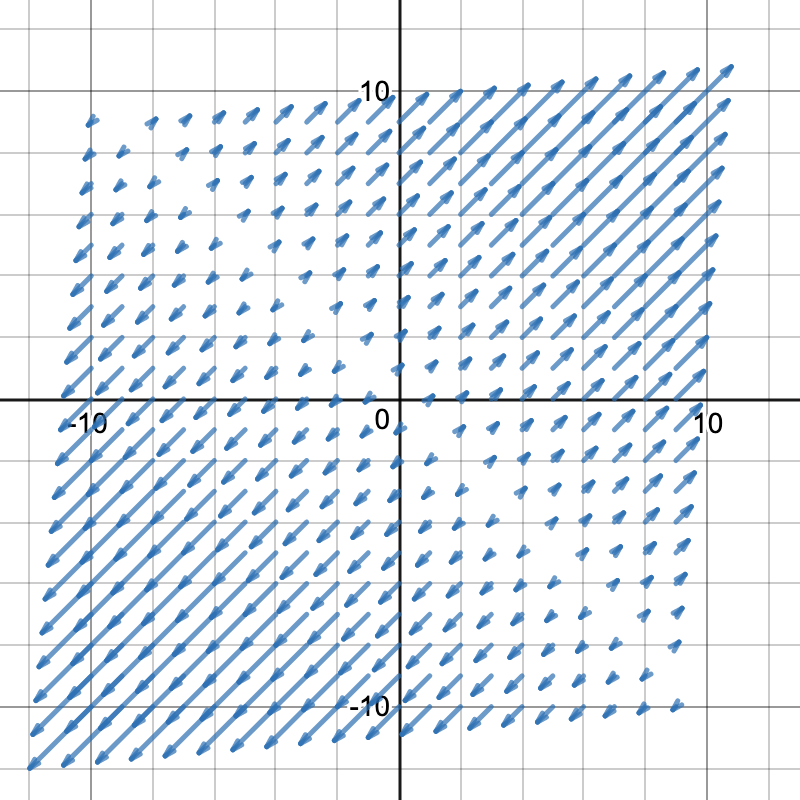
\includegraphics[width=.6\textwidth]{Figures/x+yx+y.png}
                \caption{A plot of the vector field $\mathbf{v}'(x,y)$.}
            \end{figure}
            Our goal is to then find a vector as a function of time given by
            \[
            \mathbf{v}(t) = \begin{bmatrix} x(t) \\ y(t) \end{bmatrix}
            \]
            as this will contain the solutions to our system of ODE.
            
            What we do next is pick an initial condition, $(x_0,y_0)$ and note that our vector field gives us the velocity vector $\mathbf{v}'(x_0,y_0)$ at that point. 
            
            The solution (curve/trajectory) to our system of ODE follows the vector field above since it describes the velocity of our curve at that point. We call this solution curve an \textbf{integral curve} as it is obtained (roughly) through integration of $\mathbf{v}'$.  However, you should know that it is not always possible to explicitly compute this integral.  We will learn techniques for solving certain systems, however.
            
            One should feel comfortable tracing an estimate for a solution curve for a given system as it gives a qualitative answer to the problem. In this case, if we pick a point along the line $y=-x$, the trajectory is stationary.  Otherwise, the solution follows a curve that is parallel to the $y=x$ line and the direction depends on which location it begins.
            \item We can repeat this process for another example
            \begin{align*}
                x' &= x+y,\\
                y' &= -x +y.
            \end{align*}
            This has a vector field plot:
            \begin{figure}[H]
                \centering
                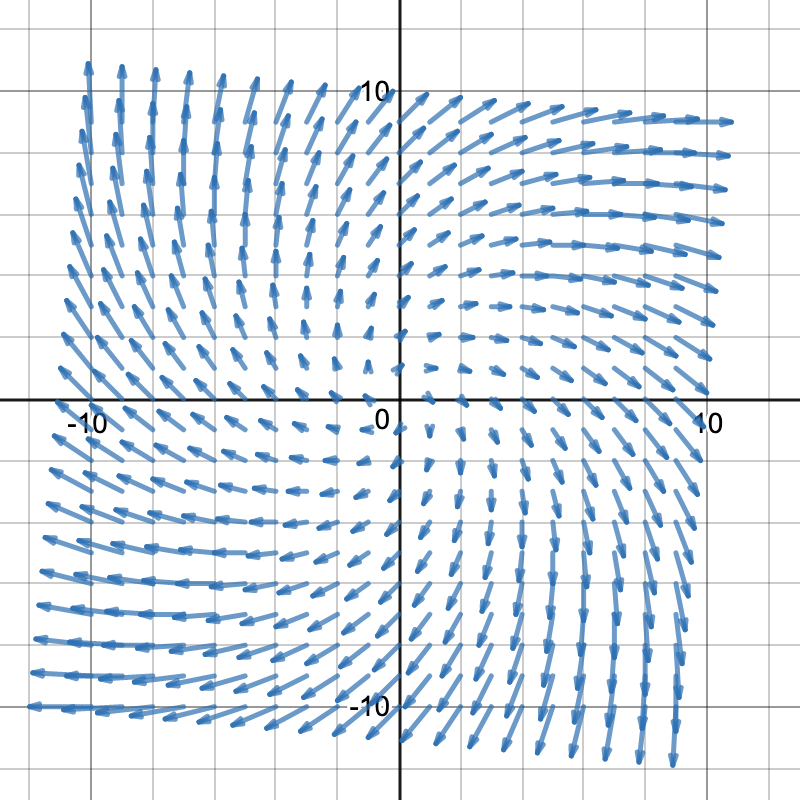
\includegraphics[width=.6\textwidth]{Figures/x+yx-y.png}
                \caption{The vector field $\mathbf{v}'(x,y)$ given by our system.}
            \end{figure}
            This solution has a stationary trajectory at the point $(0,0)$. Otherwise, the solution spirals outward in a clockwise direction. We say that this \emph{stationary point} $(0,0)$ is \emph{unstable}.
            \item Here is another example given by
            \begin{align*}
                x' &= -x +y,\\
                y' &= -x -y.
            \end{align*}
            Here is the plot of the vector field
            \begin{figure}[H]
                \centering
                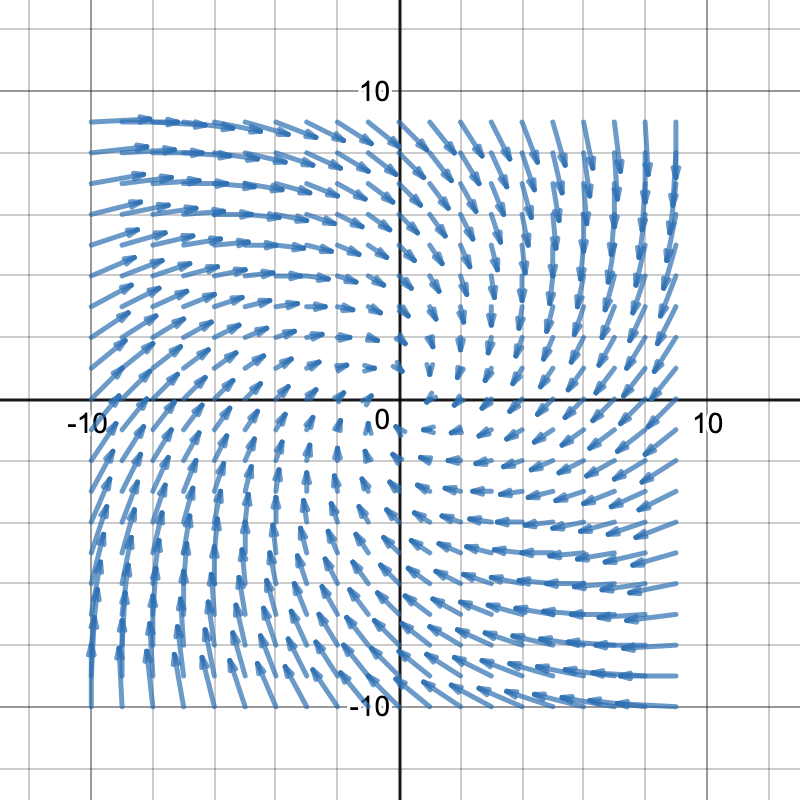
\includegraphics[width=.6\textwidth]{Figures/-x+y-x-y.png}
                \caption{The vector field $\mathbf{v}'(x,y)$ given by our system.}
            \end{figure}
            Here our solution again has a stationary trajectory at the point $(0,0)$.  Otherwise, the solution spirals inward in a clockwise direction.  Here we say that the stationary point $(0,0)$ is \emph{stable}.
            \item Let us take yet another example given by
            \begin{align*}
                x' &= y,\\
                y' &= -x.
            \end{align*}
            This has a vector field plot
            \begin{figure}[H]
                \centering
                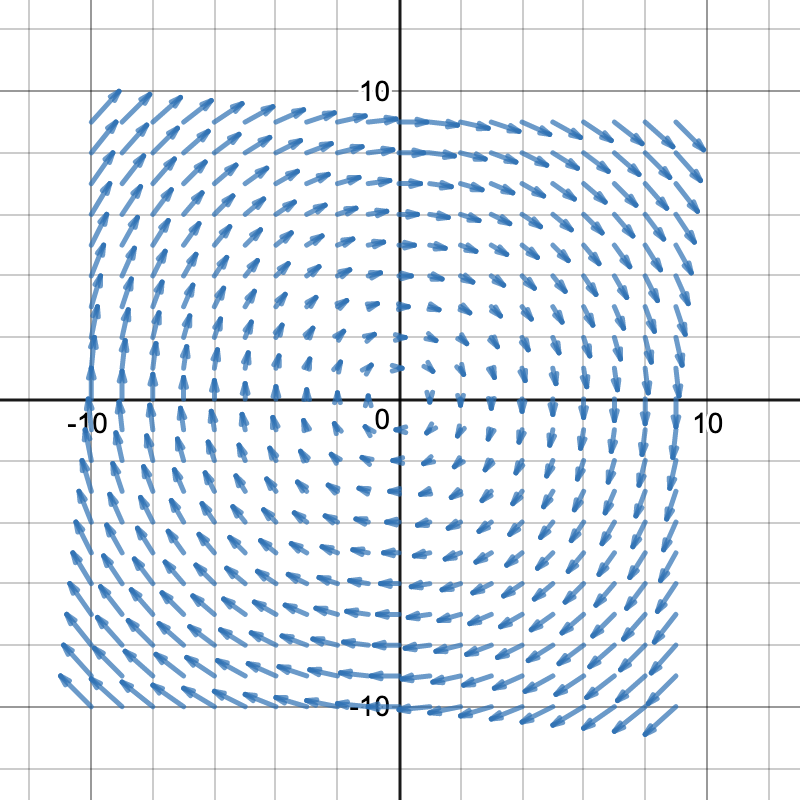
\includegraphics[width=.6\textwidth]{Figures/y-x.png}
                \caption{The vector field $\mathbf{v}'(x,y)$ given by our system.}
            \end{figure}
            Again, $(0,0)$ is a stationary point.  All the other trajectories form circles that rotate counter clockwise about the origin.
        \end{enumerate}
        \end{ex}
        
        These systems above show the four main dynamics we can see in the plane. All dynamics in the plane roughly look like one of these in close proximity to any point.
        
        \begin{ex}{General Solutions to the Zoo of Linear Systems}{gen_solns_zoo}
        We can look at the integral curves for these vector fields.  Without solving them explicitly, let's see what they would look like.
        \begin{enumerate}[(I)]
            \item The general solution for this system is
            \begin{align*}
                x(t)&= \frac{1}{2}c_1 \left( e^{2t}+1\right)+\frac{1}{2}c_2\left(e^{2t}-1\right),\\
                y(t)&=\frac{1}{2}c_1 \left( e^{2t}-1\right)+\frac{1}{2}c_2\left(e^{2t}+1\right).
            \end{align*}
            The initial data is dictated by the problem, and comes in the form of knowing $(x(0),y(0))$.  Here is a plot of a few integral curves (trajectories).
            \begin{figure}[H]
                \centering
                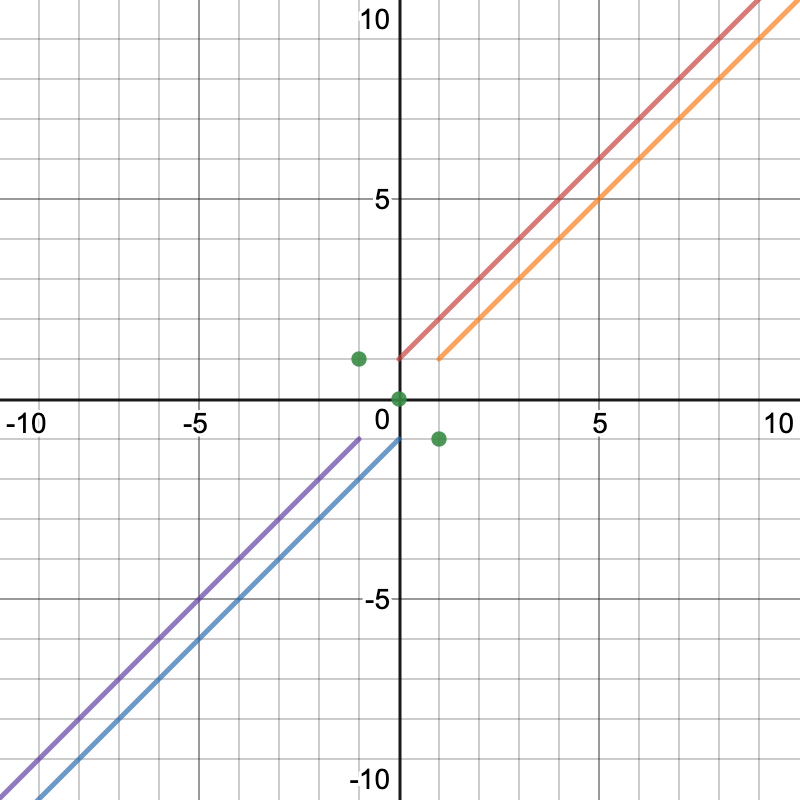
\includegraphics[width=.6\textwidth]{Figures/x+yx+yintegralcurves.png}
                \caption{Integral curves. Red: $(0,1)$; Orange: $(1,1)$; Purple: $(-1,-1)$; Blue: $(0,-1)$. Green are all stationary points.}
            \end{figure}
            \item The general solution for this system is
            \begin{align*}
                x(t)&= c_2 e^t \sin(t)+c_1e^t\cos(t),\\
                y(t)&= c_2 e^t \cos(t) - c_1e^1 \sin(t).
            \end{align*}
            Here are trajectories. Keep in mind these move radially \emph{outward} away from the stationary point!
                        \begin{figure}[H]
                \centering
                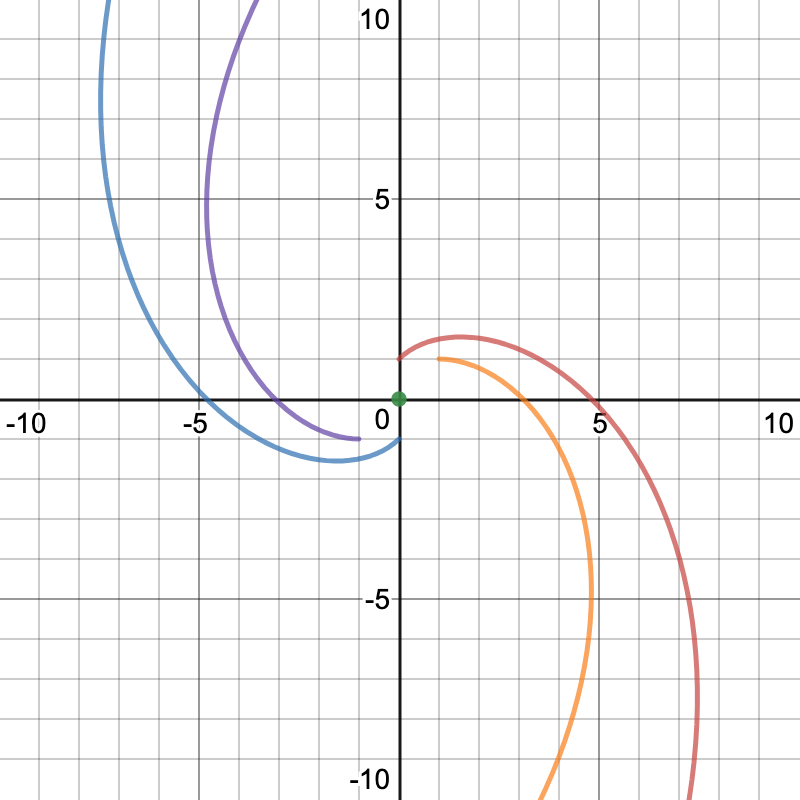
\includegraphics[width=.6\textwidth]{Figures/x+y-x+yintegralcurves.png}
                \caption{Integral curves. Red: $(0,1)$; Orange: $(1,1)$; Purple: $(-1,-1)$; Blue: $(0,-1)$. Green:$(0,0)$ is the stationary point.}
            \end{figure}
            \item The general solution for this system is
            \begin{align*}
                x(t)&=c_2 e^{-t}\sin(t)+c_1 e^{-t}\cos(t),\\
                y(t)&=c_2e^{-t}\cos(t)-c_1e^{-t}\sin(t).
            \end{align*}
            Here are trajectories. Keep in mind these are moving radially \emph{inward} towards the stationary point! Also note the difference in scale here.
            \begin{figure}[H]
                \centering
                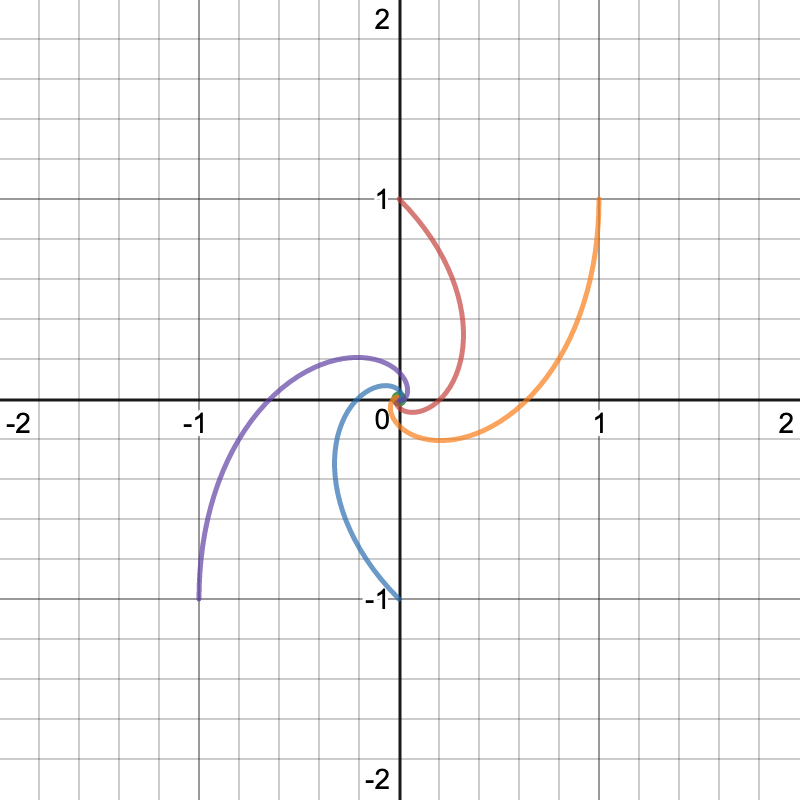
\includegraphics[width=.6\textwidth]{Figures/-x+y-x-yintegralcurves.png}
                \caption{Integral curves. Red: $(0,1)$; Orange: $(1,1)$; Purple: $(-1,-1)$; Blue: $(0,-1)$. Green: $(0,0)$ is the stationary point.}
            \end{figure}
            \item The general solution for this system is
            \begin{align*}
                x(t)&= c_2 \sin(t) + c_1 \cos(t),\\
                y(t)&= c_2 \cos(t) - c_1 \sin(t).
            \end{align*}
            Some of the trajectories here end up overlapping if we plot them over too much time.  Here's what I mean.
            \begin{figure}[H]
                \centering
                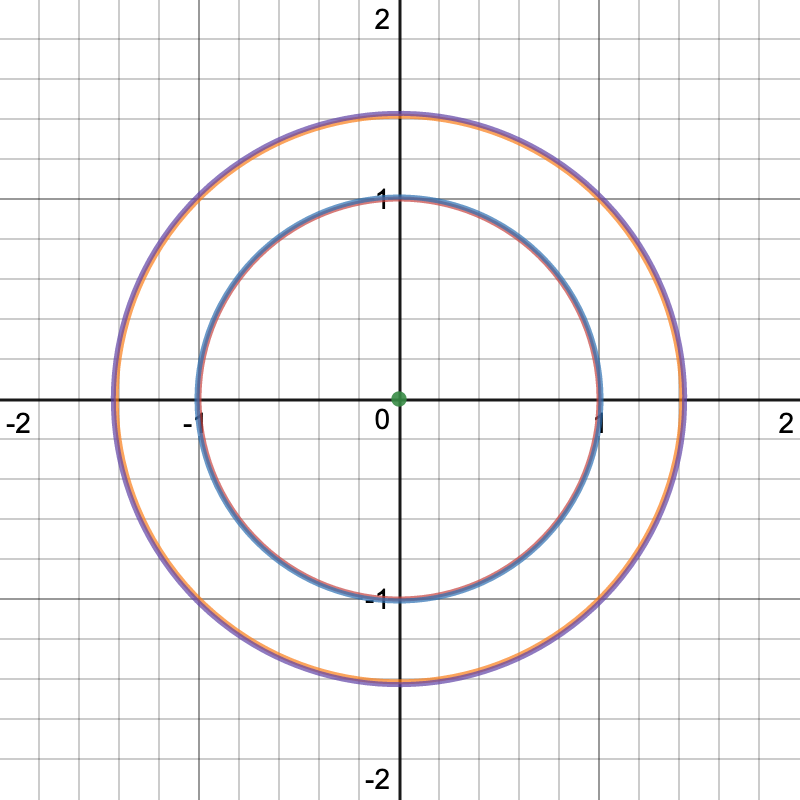
\includegraphics[width=.6\textwidth]{Figures/y-xintegralcurves.png}
                \caption{Integral curves. Red: $(0,1)$; Orange: $(1,1)$; Purple: $(-1,-1)$; Blue: $(0,-1)$. Green: $(0,0)$ is the stationary point.}
                \label{fig:my_label}
            \end{figure}
            However, here is what it looks like over a shorter period of time.
            \begin{figure}[H]
                \centering
                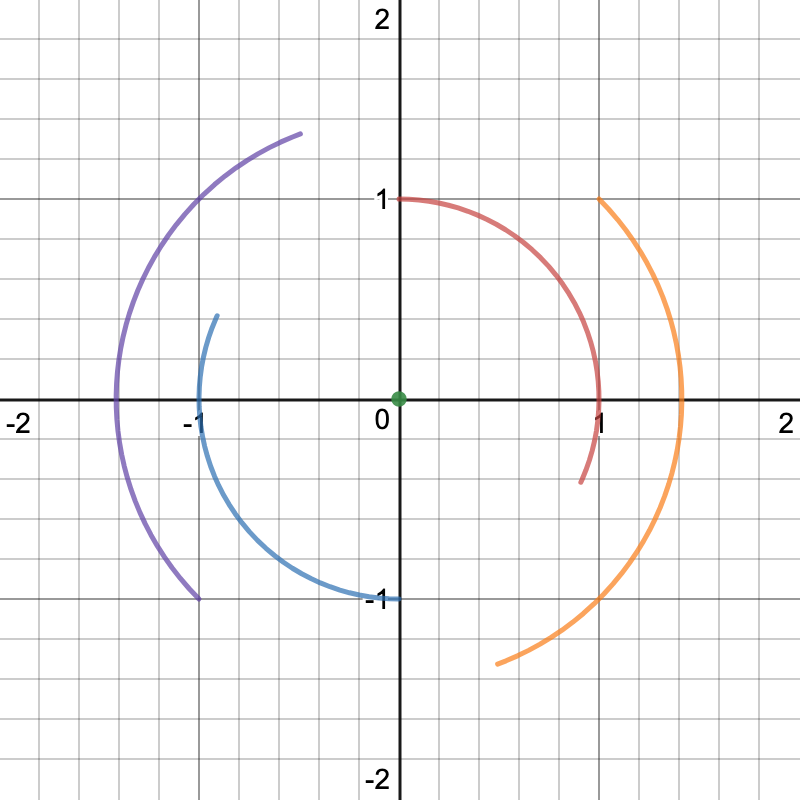
\includegraphics[width=.6\textwidth]{Figures/y-xintegralcurves2.png}
                \caption{Integral curves. Red: $(0,1)$; Orange: $(1,1)$; Purple: $(-1,-1)$; Blue: $(0,-1)$. Green: $(0,0)$ is the stationary point.}
                \label{fig:my_label}
            \end{figure}
            In a sense, each chosen initial conditions will chase one of the others forever in time.
        \end{enumerate}
        \end{ex}
        
        \section{Linearity}
        The above systems were all \emph{linear}.  These systems are in fact exactly solvable.  We'll get to the solutions shortly.  However, many systems in nature are \emph{nonlinear}.  Take for example, the SIR model. What does it mean for an ODE to be linear? 
        
        \begin{df}{Linear and Nonlinear ODE}{lin_ode}
        An $n$th order ODE is \textbf{linear} if it can take the following form
        \[
        x^{(n)}(t)+f_{n-1}(t)x^{(n-1)}(t)+\cdots + f_1(t)x'(t) +f_0(t)x(t)=g(t).
        \]
        This looks a bit complicated, so let's restate this for second order ODE.
        
        A second order $ODE$ is \textbf{linear} if it can take the following form
        \[
        x''+f(t)x'+g(t)x=h(t).
        \]
        And a first order ODE is linear if it can take the form
        \[
        x'+f(t)x=g(t).
        \]
        
        If an ODE does not satisfy the above definition, we say that it is \textbf{nonlinear}.
        \end{df}
        
        
        \section{Higher Order ODE}
        Higher order ODE show up in nature quite often.  For example, second order equations are abundant in physics due to Newton's laws.  Equations of order higher than two appear in material strain and stress (which tend to be fourth order).  
        
        The wonderful fact is that we do not need any new theory to understand higher order ODE.  This is due to the following theorem.
        
        \begin{thm}{Reduction of Order}{red_of_order}
        Any $n ^\textrm{th}$ order ODE is equivalent to a system of $n$ first order ODE.  
        \end{thm}
        
        The moral is that we need only know how to analyze first order systems in order to understand \emph{any} possible ODE.  Let's see an example of this.
        
        \begin{ex}{Order Reducing the Harmonic Oscillator}{order_red_harm_osc}
        Consider the harmonic oscillator equation
        \[
        x''=-x.
        \]
        We can define a new variable, $v$ so that $v=x'$.  Then note we have that $v'=x''$.  Substituting these gives us two first order equations
        \begin{align*}
            x'&=v,\\
            v'&=-x.
        \end{align*}
        It may seem like we have essentially done nothing.  But we've actually changed the problem for the better.  We'll see why soon.
        \end{ex}
        
        \begin{ex}{The Biharmonic Equation}{biharmonic_eq}
        Consider the \emph{biharmonic equation}
        \[
        x''''=x.
        \]
        We can define a set of new variables $y=x'$, $z=y'$, and $w=z'$.  Note that $w'=z''=y'''=x''''$. Then we arrive at the system
        \begin{align*}
            x'&=y,\\
            y'&=z,\\
            z'&=w,\\
            w'&=x.
        \end{align*}
        We have turned a fourth order ODE into a system of four first order ODE.
        \end{ex}
        
        \section{Linear Systems}
        Let's say we are given a nonlinear higher order ODE or system. We wish to be able to convert this to a linear problem of the form 
        \[
        \mathbf{v}'=A\mathbf{v}+\mathbf{F}
        \]
        where, for example, 
        \[
        \mathbf{v}=\begin{bmatrix} x(t) \\ y(t) \\ z(t) \end{bmatrix} \qquad \mathbf{v}'=\begin{bmatrix} x'(t) \\ y'(t) \\ z'(t) \end{bmatrix} \qquad \begin{bmatrix} f_1(t) \\ f_2(t) \\ f_3(t) \end{bmatrix}.
        \]
        We call this the \emph{inhomogeneous} system. 
        
        Roughly speaking, we can think of $\mathbf{F}$ as an external forcing term acting on the system.  We will concentrate more on solving the case where $\mathbf{F}=\mathbf{0}$ so that we have
        \[
        \mathbf{v}'=A\mathbf{v}.
        \]
        We call this the \emph{homogeneous} system. Here, $A$ is a $3\times 3$-matrix whose coefficients could possibly depend on time.  That is,
        \[
        A = \begin{bmatrix} A_{11}(t) & A_{12}(t) & A_{13}(t)\\
        A_{21}(t) & A_{22}(t) & A_{23}(t)\\
        A_{31}(t) & A_{32}(t) & A_{33}(t)\end{bmatrix}.
        \]
        We will ignore the case where the matrix depends on time and just work on the case where the coefficients are constant. This is called an \emph{autonomous} system.
        
        \begin{df}{Linear System of ODE}{linear_system}
            A system of first order differential equations is \textbf{linear} if it can be expressed as a matrix equation
            \[
            \mathbf{v}' = A(t)\mathbf{v}+\mathbf{F}(t).
            \]
            The linear system is said to have \textbf{constant coefficients} if the matrix $A(t)$ only contains constant.  That is, $A$ does not actually depend on $t$.
        \end{df}
        
        \begin{df}{Homogeneous and Inhomogeneous Linear Systems}{homogeneous_systems}
            A linear system of differential equations is 
            \textbf{inhomogeneous} if it can be expressed as
            \[
            \mathbf{v}' = A(t)\mathbf{v}+\mathbf{F}(t).
            \]
            If $\mathbf{F}(t)=0$ and we have
            \[
            \mathbf{v}' = A(t)\mathbf{v}
            \]
            then we say the system of differential equations is \textbf{homogeneous}.
        \end{df}
        
        \begin{df}{Autonomous}{autonomous}
        An \textbf{autonomous} first order system (in 3-dimensions) is given by the equations
        \begin{align*}
        x' &= f(x,y,z),\\
        y' &= g(x,y,z),\\
        z' &= h(x,y,z).
        \end{align*}
        This is autonomous due to the fact that $t$ does not appear as an argument for the functions $f,g,$ and $h$.
        \end{df}
        
        Autonomous systems are extremely common in reality which is why it is not a bad idea to emphasize them here.  These are the systems in which some quantity is being conserved over time, and hence the apparent $t$ dependence of the functions (shown above) is gone.  Of course, the functions still depend on $t$!  A few examples are
        \begin{itemize}
            \item mechanical systems (energy is conserved),
            \item closed thermodynamic systems (energy is conserved),
            \item short time ecologocial systems (animal number is conserved), 
            \item closed chemically reacting systems (total atomic count is constant).
        \end{itemize}
        
        For us, we are going to concentrate on dynamics for a system of two equations.  That is, equations that exist in the plane.  For one, these systems are easier to solve by hand than the higher dimensional systems.  They are also very common to see due again to Newton's laws.  Often, we will find we can decompose larger systems of equations into sets of systems of two equations. Lastly, these are likely the easiest to visualize and build intuition with.  
        
        \section{Linearization}
        If we are given a planar (autonomous) and possibly nonlinear system, 
        \begin{align*}
            x'&= f(x,y),\\
            y'&= g(x,y),
        \end{align*}
        we want to approximate this system with a homogeneous linear system with a matrix with constant coefficients.  That is
        \[
        \begin{bmatrix} x' \\ y' \end{bmatrix} \approx \begin{bmatrix} A_{11} & A_{12} \\ A_{21} & A_{22} \end{bmatrix} \begin{bmatrix} x \\ y \end{bmatrix}.
        \]
    
        Remember that what we have here is a 2-dimensional vector field given by our system
        \[
        \mathbf{v}(x,y) = \begin{bmatrix} f(x,y) \\ g(x,y) \end{bmatrix}.
        \]
        The best linear approximation to this vector field at a point $(x_0,y_0)$ is given by the Jacobian $J(x_0,y_0)$ for this vector field
        \[
        J(x_0,y_0) = \begin{bmatrix} \frac{\partial f}{\partial x}(x_0,y_0) & \frac{\partial f}{\partial y}(x_0,y_0) \\
        \frac{\partial g}{\partial x}(x_0,y_0) & \frac{\partial g}{\partial y}(x_0,y_0) \end{bmatrix}.
        \]
        We will then let the coefficient matrix be given by this Jacobian.  That is, we get
        \[
        \begin{bmatrix} x' \\ y' \end{bmatrix} = J(x_0,y_0)\begin{bmatrix} x \\ y \end{bmatrix}.
        \]
        Let's work an example.
        
        \begin{ex}{Lotka-Volterra Model Linearization}{lotka_volterra_linearization}
        Let us consider a predator and prey system given by the Lotka-Volterra model.  Here we let the number of prey be given by $R(t)$ and the number of predators be given by $S(t)$.  The system is
        \begin{align*}
            S' &= (-c+dR)S,\\
            R' &= (a-bS)R,
        \end{align*}
        where $a,b,c,d>0$. Here we can say that we have
        \begin{align*}
        f(S,R) &= (-c+dR)S,\\
        g(S,R) &= (a-bS)R.
        \end{align*}
        We compute each partial derivative
        \begin{align*}
            \frac{\partial f}{\partial S} &= -c+dR & \frac{\partial f}{\partial R} &=dS \\
            \frac{\partial g}{\partial S} &= -bR & \frac{\partial g}{\partial R} &= a-bS.
        \end{align*}
        Evaluating each at the point $(S_0,R_0)$ and placing into a matrix gives us the Jacobian
        \[
        J(S_0,R_0)=\begin{bmatrix} -c+dR_0 & dS_0 \\ -bR_0 & a-bS_0 \end{bmatrix}.
        \]
        
        Now, about this point, our system approximately takes the form
        \[
        \begin{bmatrix} S' \\ R' \end{bmatrix} = \begin{bmatrix} -c+dR_0 & dS_0 \\ -bR_0 & a-bS_0 \end{bmatrix} \begin{bmatrix} S \\ R \end{bmatrix}.
        \]
        \end{ex}
        
        Our goal now is to learn how we can explicitly solve these planar systems.  With that, we will be able to solve many problems.
        
        
        Now that we can take many common ODE, convert them to a system of first order ODE, and linearize the system, we can work to solve these specific equations.  The detail is captured by the following.
        
        \begin{prop}{Eigenfunction of the Derivative}{eigenfunction}
        The exponential function $e^{kx}$ is an \textbf{eigenfunction} for the derivative.  \\
        
        \noindent \emph{Proof.} We take 
        \[
        \frac{d}{dt} e^{kt} = ke^{kt}.
        \]
        So, the eigenvalue is $k$ for this eigenfunction. \qed
        \end{prop}
        
        
        Spending the time being more rigorous with this is an interesting endeavor, but we have done enough theoretical results for now.  Let us see an example.
        
        \begin{ex}{Harmonic Oscillator Eigenvalue}{harm_osc_eigen}
        If we take the Harmonic Oscillator equation
        \[
        x'' = -x
        \]
        we can realize this extremely similar to an eigen equation with
        \[
        x'=ix.
        \]
        So, this eigen equation has a solution
        \[
        x(t)=e^{it}.
        \]
        Note that this solves the Harmonic oscillator equation since
        \[
        \frac{d^2}{dt^2} x(t) = \frac{d}{dt}ie^{it} = -e^{it}=-x.
        \]
        Remember that
        \[
        e^{it}=\cos(t)+i\sin(t)
        \]
        which captures the oscillating behavior.
        \end{ex}
        
        In short, these exponential functions capture oscillations, growth, and decay.  With these functions, we can model all linear systems.
        
        \begin{prop}{General Solution to Planar Linear Systems}{gen_soln_lin_systems}
        Given a two dimensional linear system with constant coefficients $A,B,C$, and $D$,
        \begin{align*}
        x' &= Ax+By,\\
        y' &= Cx+Dy,
        \end{align*}
        we can write this as a matrix equation
        \[
        \begin{bmatrix} x' \\ y' \end{bmatrix} = \begin{bmatrix} A & B\\ C & D \end{bmatrix} \begin{bmatrix} x \\ y \end{bmatrix},
        \]
        with
        \[
        M=\begin{bmatrix} A & B \\ C & D \end{bmatrix}.
        \]
        Let $\lambda_1$ and $\lambda_2$ be the (complex) eigenvalues of $M$ and $\mathbf{v}_1$ and $\mathbf{v}_2$ be the corresponding eigenvectors.  Then, the solution to the system of equations is
        \[
        \begin{bmatrix} x(t) \\ y(t) \end{bmatrix} = c_1 \mathbf{v}_1 e^{\lambda_1t} + c_2 \mathbf{v}_2e^{\lambda_2 t}.
        \]
        \end{prop}
        
        Let us unravel this with an example problem.
        
        \begin{ex}{Damped Harmonic Motion}{damped_harm_motion}
        Consider the Damped Harmonic Oscillator equation
        \[
        x'' +\mu x' + kx = 0,
        \]
        with initial data $x(0)=1$ and $x'(0)=0$.\\ 
        
        Let us first think about this problem with our intuition.  This equation is modelling a spring mass system that is in a damping medium (i.e., underwater).  What happens as this system evolves?  One should expect oscillation, but will the system oscillate indefinitely? No.  One should expect that this system will also begin to oscillate with less intensity over time.  With this, one could hazard a guess that
        \[
        x(t) \approx e^{-t}\cos(t).
        \]
        
        We can reduce the order of this equation by letting $y=x'$.  This gives us the system
        \begin{align*}
        x' &= y,\\
        y' &= -kx -\mu y.
        \end{align*}
        So we can write this as a matrix equation
        \[
        \begin{bmatrix} x' \\ y' \end{bmatrix} = \begin{bmatrix} 0 & 1 \\ -k & -\mu \end{bmatrix}.
        \]
        For simplicity, let $k=\mu=1$, and we get the matrix
        \[
        M = \begin{bmatrix} 0 & 1 \\ - 1& - 1 \end{bmatrix}.
        \]
        Then the eigenvalues to this matrix are
        \[
        \lambda_1 = \frac{1}{2}(-1+i\sqrt{3})\quad \textrm{and} \quad \lambda_2 = \frac{1}{2}(-1-i\sqrt{3}).
        \]
        The eigenvectors are
        \[
        \mathbf{v}_1 = \begin{bmatrix} \frac{1}{2} (-1-i\sqrt{3}) \\ 1 \end{bmatrix} \quad \textrm{and} \quad \mathbf{v}_2 = \begin{bmatrix} \frac{1}{2} (-1+i\sqrt{3}) \\ 1 \end{bmatrix}.
        \]
        By the proposition, our solution is
        \[
        \begin{bmatrix} x(t) \\ y(t) \end{bmatrix} = c_1 \begin{bmatrix} \frac{1}{2} (-1-i\sqrt{3}) \\ 1 \end{bmatrix} e^{\frac{1}{2}(-1+i\sqrt{3})t}+c_2  \begin{bmatrix} \frac{1}{2} (-1+i\sqrt{3}) \\ 1 \end{bmatrix} e^{\frac{1}{2}(-1-i\sqrt{3})t}.
        \]
        However, in this case we are wishing to just find $x(t)$ that fits this data, and what we find is this system of equations reduces to
        \begin{align*}
        x(t) &= c_1 e^{\frac{1}{2}(-1+i\sqrt{3})t}+c_2 e^{\frac{1}{2}(-1-i\sqrt{3})t},
        \end{align*}
        by looking at just the first entry of each vector and realizing that since $c_1$ and $c_2$ are undetermined constants, we can remove the other constants that appear.
        
        Now, let's use Euler's formula, and we have
        \begin{align*}
            x(t) &= c_1 e^{\frac{1}{2}(-1+i\sqrt{3})t}+c_2 e^{\frac{1}{2}(-1-i\sqrt{3})t}\\
            &= c_1 e^{-t/2}\left(\cos\left(\frac{\sqrt{3}}{2}t\right)+i\sin\left(\frac{\sqrt{3}}{2}t\right)\right)+c_2 e^{-t/2}\left(\cos\left(-\frac{\sqrt{3}}{2}t\right)+i\sin\left(-\frac{\sqrt{3}}{2}t\right)\right).
        \end{align*}
        There are a few more simplifications that can be done, but in the end we find the general solution
        \[
        x(t) = c_1 e^{-t/2} \sin\left(\frac{\sqrt{3}}{2}t\right)+c_2e^{-t/2}\cos\left(\frac{\sqrt{3}}{2}t\right).
        \]
        We were given that $x(0)=1$ and we have that
        \[
        x(0)=1=c_2
        \]
        by plugging into our general solution.  We also have that
        \[
        x'(0)=0=\frac{-\sqrt{3}}{4}c_1
        \]
        which means $c_1=0$.  So our particular solution is
        \[
        x_p(t) = e^{-1/2t}\cos \left(\frac{\sqrt{3}}{2}t\right).
        \]
        
        This solution also seems fit our physical expectations of the damped spring-mass system.  Great!
        \end{ex}
        
        \begin{exercise}
        Verify that this $x_p$ above is indeed a solution to the original ODE with $k=\mu=1$.
        \end{exercise}

        \begin{remark}
        The apparent difficulty of solving ODEs becomes obvious here.  In this extremely nice case it still took a large amount of work.  The case for other systems is generally worse.
        \end{remark}
        
        \section{General Solutions to Second Order Linear Equations}
        
        We can now write the general solutions to all second order linear equations.  We have the following.
        
        \begin{prop}{General Solutions to Second Order Linear Equations}{gen_solns_second_order}
        Given a second order homogeneous linear ODE
        \[
        x'' + \mu x' + kx = 0
        \]
        we can write this as a system of first order linear equations given by
        \[
        \mathbf{v}' = M \mathbf{v},
        \]
        where
        \[
        \mathbf{v} = \begin{bmatrix} x \\ y \end{bmatrix}.
        \]
        the eigenvalues of $M$ are either purely real or complex.
        
        \begin{itemize}
            \item If the eigenvalues $\lambda_1$ and $\lambda_2$ are complex, then the solution is
        \[
        x(t)= c_1 e^{\RE(\lambda_1)t} \sin(\IM(\lambda_1)t) + c_2 e^{\RE(\lambda_1)t} \sin(\IM(\lambda_1)t).
        \]
        It does not actually matter if we choose $\lambda_1$ or $\lambda_2$!
        \item         If the eigenvalues $\lambda_1$ and $\lambda_2$ are real then the general solution is:
        \[
        x(t) = c_1 e^{\lambda_1 t} + c_2 e^{\lambda_2 t}.
        \]
        \end{itemize}
        \end{prop}

    \textcolor{red}{Add in Noether's theorem for ODEs and groups, a little bit of vector fields and stuff?}


        We now want to investigate a larger class of differential equations.  These are the \boldgreen{partial differential equations} or PDEs.  These equations become yet more complicated to solve, but are very prevalent in the study of the physical world.
        
        Fundamentally, these are time-varying differential equations of vector and scalar fields of many variables.  The goal for us is to be able to recognize a few specific example equations and understand their behavior.  We will also be able to solve a few equations with our tools from studying ODE. However, it is easy to pose a PDE that is virtually impossible to solve.  
        
        \begin{df}{Partial Differential Equation}{pde}
        A \boldgreen{partial differential equation of a scalar field} of three spatial variables $x,y,z$ and a time variable $t$ is an expression of a scalar function $u(x,y,z,t)$, the partial derivatives of $u(x,y,z,t)$, and other functions.
        \end{df}
        
        \begin{df}{Vector Partial Differential Equation}{vec_pde}
        A \boldgreen{partial differential equation of a vector field}
        \[
        \vecfieldV(x,y,z,t) = \begin{bmatrix} V_1(x,y,z,t) \\ V_2(x,y,z,t) \\ V_3(x,y,z,t) \end{bmatrix}
        \]
        is an equation containing $\vecfieldV$, the (component) derivatives of $\vecfieldV$, and other vector fields.
        \end{df}
        
        With the difficulty of these expressions as is, we will concentrate solely on the equations with scalar functions.
    % %%%%%%%%%%%%%%%%%%%%%%%%%%%%%%%%%%%%%%%%%%%%%%%%%%%%%%%%%%%%%%%%%%%%%%%%%%%%%%%%%%%%
    % Examples of PDE
    % %%%%%%%%%%%%%%%%%%%%%%%%%%%%%%%%%%%%%%%%%%%%%%%%%%%%%%%%%%%%%%%%%%%%%%%%%%%%%%%%%%%%
    
        \section{Examples of PDE}
        
        \begin{ex}{Heat Equation}{heat_eqn}
        The \boldgreen{linear heat equation} in three dimensional space is the equation
        \[
        \frac{\partial u}{\partial t}(x,y,z,t) -k\nabla \cdot (\nabla u(x,y,z,t)) = f(x,y,z,t).
        \]
        This equation models the diffusion of heat in a region of space, hence the name.  In this case, we think of $u(x,y,z,t)$ being the temperature at the point $(x,y,z)$ at the time $t$.
        \end{ex}
        
        \begin{ex}{Laplace (Poisson) Equation}{laplace}
        The \boldgreen{Laplace} (sometimes \boldgreen{Poisson}) \boldgreen{equation} in three dimensional space is the equation
        \[
        -\Delta=-\nabla \cdot (\nabla u(x,y,z))=f(x,y,z).
        \]
        \emph{Notice, there is no dependence on time!} This equation is the long term behavior of the heat equation.  If $u(x,y,z)$ describes temperature, then the solution to this equation tells you the equilibrium temperature. Since this is an equilibrium solution, the time component is gone.
        \end{ex}
        
        \begin{ex}{The Wave Equation}{wave}
        The \boldgreen{linear wave equation} in three dimensional space is the equation
        \[
        \frac{\partial^2 u}{\partial^2 t}(x,y,z,t) -c^2\Delta \cdot (\nabla u(x,y,z,t)) = f(x,y,z,t).
        \]
        The solutions here are wavelike.  Think of plucking a guitar string, or the ripples on the surface of a lake after a rock has been tossed in, or the vibrating cymbal or drum head.
        \end{ex}
        
        \begin{ex}{Maxwell's Equations}{maxwell}
        Maxwell's equations describe the electric $\vecfieldE$ and magnetic $\vecfieldB$ fields that permeate space due to charged particles.  These equations turn out to be coupled PDE.  They read
        \begin{align*}
            \grad \cdot \vecfieldE(x,y,z,t) &= \frac{\rho(x,y,z,t)}{\epsilon},\\
            \grad \cdot \vecfieldB(x,y,z,t) &= 0,\\
            \grad \times \vecfieldE(x,y,z,t) &= -\frac{\partial \vecfieldB}{\partial t}(x,y,z,t),\\
            \grad \times \vecfieldB(x,y,z,t) &= \mu \vecfieldJ + \mu \epsilon \frac{\partial \vecfieldE}{\partial t}(x,y,z,t).
        \end{align*}
        \end{ex}
        
        \section{The Problem Statement}
        
        In order to move forward, we need to also properly specify the problem we want to solve.
        
        The one-dimensional source-free heat equation is a great starting point to begin our process.  We are given the following data:
        \begin{itemize}
            \item A region $\Omega$ in space that we are concerned with.  For example, in one dimension, we can consider the interval $\Omega=(0,1)$.
            \item A PDE
            \[
            \frac{\partial u}{\partial t}(x,t) -k \frac{\partial^2 u}{\partial x}^2 = 0.
            \]
            \item Boundary conditions. These can come in a few forms, but we will concentrate on just one. We must specify $u(0,t)=a$ and $u(1,t)=b$.  These boundary conditions correspond to fixing the temperature at the ends of a rod constant.
            \item Initial conditions. We specify the initial temperature distribution
            \[
            u(x,0)=u_0(x).
            \]
        \end{itemize}
    
    % %%%%%%%%%%%%%%%%%%%%%%%%%%%%%%%%%%%%%%%%%%%%%%%%%%%%%%%%%%%%%%%%%%%%%%%%%%%%%%%%%%%%
    % The Heat Equation
    % %%%%%%%%%%%%%%%%%%%%%%%%%%%%%%%%%%%%%%%%%%%%%%%%%%%%%%%%%%%%%%%%%%%%%%%%%%%%%%%%%%%%
    
        \section{The Heat Equation}
        One of the most illuminating examples of PDEs is the heat equation.  Let us work through a specific example of the heat equation and keep in mind the physical intuition throughout.
        
        \begin{ex}{Solving the Heat Equation}{solving_heat_equation}
        Let us consider the simplified one-dimensional source free (i.e., the right hand side is zero) heat equation given by the following:
        \[
        \frac{\partial u}{\partial t}(x,t)-\frac{\partial^2 u}{\partial x^2} = 0.
        \]
        We can require boundary conditions and initial conditions later on.\\
        
        Let us assume that the solution function $u(x,t)$ can be written as
        \[
        u(x,t) = f(x)g(t).
        \]
        We call this approach the \boldgreen{separation of variables}. We then plug in this assumption to our PDE.
        \begin{align*}
            \frac{\partial}{\partial t} (f(x)g(t))-\frac{\partial^2}{\partial x^2} (f(x)g(t)) &= 0\\
            f(x)\frac{\partial g}{\partial t}-g(t)\frac{\partial^2 f}{\partial x^2}&=0\\
            fg'-f''g &=0.
        \end{align*}
        We can then do a bit more algebra.
        \begin{align*}
            fg'-f''g&=0\\
            fg'&= f''g\\
            \frac{g'(t)}{g(t)}&=\frac{f''(x)}{f(x)}.
        \end{align*}
        Now, notice that both sides depend on different variables.  We have successfully separated this equation into an equation for each variable.  This is to say, since each side of the equation depends on a different variable, each side must be equal to a constant $\lambda$! So we have two equations.
        \begin{align*}
            \frac{g'(t)}{g(t)}&=\lambda\\
            \frac{f''(x)}{f(x)}&=\lambda.
        \end{align*}
        We can then solve both of these as ODE. Note, it will be helpful to to instead choose $-\lambda$ as the constant.
        \end{ex}
        
        \begin{exercise}
        What are the general solutions to the above ODE?
        \end{exercise}
        
        \begin{exercise}
        Given those general solutions, what is the general solution to the heat equation?
        \end{exercise}
        
        \begin{answer}
        We get
        \[
        \boxed{u(x,t)=f(x)g(t) = Ae^{-\lambda t}\sin(\sqrt{\lambda}t)+Be^{-\lambda t}\cos(\sqrt{\lambda}t).}
        \]
        \end{answer}
        
        Previously we found the general solution to the heat equation 
        \[
        \frac{\partial u}{\partial t}(x,t) - \frac{\partial^2 u}{\partial x^2} (x,t) = 0
        \]
        is
        \[
        u(x,t)=Ae^{-\lambda t}\sin(\sqrt{\lambda}x)+Be^{-\lambda t}\cos(\sqrt{\lambda}x).
        \]
        However, this solution is very general.  We have the undetermined constants $\lambda$, $A$, and $B$. We need more information to get a particular solution.
        
        \begin{ex}{Particular Solution to the 1D Heat Equation}{particular_heat}
        We will stick with the one-dimensional case but we must pick the following.  
        \begin{itemize}
            \item Domain: Let $\Omega = (0,1)$.
            \item Initial Conditions: $u(x,0)=\sin(\pi x)$.
            \item Boundary Conditions: $u(1,t)=u(0,t)=0$.  
        \end{itemize}
        This list of requirements gives us enough information to solve the equation explicitly for a particular solution.\\
        
        First, let us take the boundary conditions. We impose these on our general solution:
        \[
        u(x,t)=Ae^{-\lambda t}\sin(\sqrt{\lambda}x)+Be^{-\lambda t}\cos(\sqrt{\lambda}x).
        \]
        Thus we require
        \[
        0=u(0,t)=Ae^{-\lambda t}\sin(0)+Be^{-\lambda t}\cos(0)
        \]
        which gives us that
        \[
        B=0.
        \]
        The other boundary condition is
        \[
        0=u(1,t)=Ae^{-\lambda t}\sin(\sqrt{\lambda}).
        \]
        Specifically, this means that $A=0$, which gives us a trivial solution or that we have
        \[
        \sqrt{\lambda}=n\pi
        \]
        for any integer $n$.  This is because $\sin(n\pi)=0$ when $n$ is an integer. Thus our solution now reads
        \[
        u(x,t)=Ae^{-n^2\pi^2}\sin(n\pi x).
        \]
        
        Lastly, we match our initial conditions.  So we have
        \[
        \sin(\pi x)=u(x,0)=A e^0 \sin(n\pi x)
        \]
        and so we find that $n=1$.  Thus, our solution is
        \[
        \boxed{u(x,t)=e^{-\pi^2 t} \sin(\pi x).}
        \] 
        
        We can plot this solution as follows.
        \begin{figure}[H]
        	\centering
        	\def\svgwidth{0.75\columnwidth}
        	\input{Figures_Part_7/heat_solution.pdf_tex}
        \end{figure}
        \end{ex}
        
        \begin{exercise}
        Can you interpret what this is physically describing as $t$ gets larger?
        \end{exercise}
        
    % %%%%%%%%%%%%%%%%%%%%%%%%%%%%%%%%%%%%%%%%%%%%%%%%%%%%%%%%%%%%%%%%%%%%%%%%%%%%%%%%%%%%
    % The Laplace Equation
    % %%%%%%%%%%%%%%%%%%%%%%%%%%%%%%%%%%%%%%%%%%%%%%%%%%%%%%%%%%%%%%%%%%%%%%%%%%%%%%%%%%%%
    
        \section{The Laplace Equation}
        In the long time limit ($t\to \infty$) or steady-state of the (source free) heat equation, one arrives at the so called Laplace equation
        \[
        -\Delta u = 0.
        \]
        In the one-dimensional case, this equation reads
        \[
        -\frac{d^2 u}{dx^2}(x) = 0.
        \]
        Note there is no dependence on time as this is the steady-state behavior for the heat equation.
        
        \begin{exercise}
        This is an ODE in the variable $x$.  You can solve this and find a general solution by integration.  
        \end{exercise} 
        
        \begin{answer}
        The general solution to the one-dimensional Laplace equation is the equation for a line
        \[
        u(x) = Ax+B.
        \]
        One can show that this is indeed a solution by taking two derivatives of $u(x)$ and finding that you get zero.
        \end{answer}
        
        \begin{ex}{Particular Solution to the 1D Laplace Equation}{particular_laplace}
        Through integration, we find
        \[
        u(x) = Ax+B
        \]
        where $A$ and $B$ are undetermined constants.  In order to specify these constants, we must provide the following.
        \begin{itemize}
            \item Domain: Let $\Omega = (0,1)$.
            \item Boundary Conditions: $u(0)=0$ and $u(1)=0$.  
        \end{itemize}
        Note that we do not need initial conditions since there is no time dependence in this PDE.\\
        
        Now, to find the particular solution, we apply the boundary conditions to our general solution.  So we have
        \[
        0=u(0)=A(0)+B,
        \]
        so $B=0$.  Then the other condition 
        \[
        0=u(1)=A,
        \]
        so $A=0$.  Thus, our solution is
        \[
        \boxed{u(x)=0}.
        \]
        Now, compare this to the solution to the heat equation previously
        \[
        u(x,t)=e^{-\pi^2 t}\sin(\pi x).
        \]
        We claimed the Laplace equation is the long-time solution of the heat equation and indeed if we look at $t\to\infty$, we have
        \[
        \lim_{t\to \infty} u(x,t)=0.
        \]
        \end{ex}
        
    % %%%%%%%%%%%%%%%%%%%%%%%%%%%%%%%%%%%%%%%%%%%%%%%%%%%%%%%%%%%%%%%%%%%%%%%%%%%%%%%%%%%%
    % The Wave Equation
    % %%%%%%%%%%%%%%%%%%%%%%%%%%%%%%%%%%%%%%%%%%%%%%%%%%%%%%%%%%%%%%%%%%%%%%%%%%%%%%%%%%%%

        \section{The Wave Equation}
        The wave equation is studied when one wants to find the oscillatory behavior of some medium.  For example, one can pluck a guitar string or hit a drum head.  These actions induce vibrations in the medium (the string or head) and it is the vibrations that one hears.  The equation that models these phenomenon is the wave equation
        \[
        \frac{\partial^2 u}{\partial t^2}(x,y,z,t)-c^2 \nabla \cdot \nabla u(x,y,z,t)=f(x,y,z,t).
        \]
        
        \begin{ex}{Solving the 1D Wave Equation}{1d_wave}
        In one-dimension, the simplified source free wave equation reads
        \[
        \frac{\partial^2 u}{\partial t^2}(x,t) -\frac{\partial^2 u}{\partial x^2}(x,t)=0.
        \]
        
        It turns out we can solve the 1D wave equation in the same way we did the heat equation. So, we assume a separation of variables approach in that 
        \[
        u(x,t) = f(x)g(t).
        \]
        We plug this into the PDE to find
        \begin{align*}
            \frac{\partial^2}{\partial t^2}(f(x)g(t))-\frac{\partial^2}{\partial x^2}(f(x)g(t))&=0\\
            f(x)\frac{\partial^2 g}{\partial t^2}-g(t)\frac{\partial^2 f}{\partial x^2}&=0\\
            f(x)g''(t)-f''(x)g(t)&=0.
        \end{align*}
        We then wish to make the left hand side and right hand side functions of different input variables
        \begin{align*}
            f(x)g''(t)-f''(x)g(t)&=0\\
            f(x)g''(t)&=f''(x)g(t)\\
            \frac{g''(t)}{g(t)}&= \frac{f''(x)}{f(x)}.
        \end{align*}
        Since each side depends on a different input variable, each side must be equal to a constant.  So this gives us
        \[
        \frac{g''(t)}{g(t)}= \frac{f''(x)}{f(x)}= -\lambda^2,
        \]
        where $-\lambda^2$ is an undetermined constant but was chosen to make the next steps easier. We then get two ODEs
        \begin{align*}
            f''(x)&=-\lambda^2 f(x),\\
            g''(t)&=-\lambda^2 g(t),
        \end{align*}
        which are both harmonic oscillator equations.  Thus, since we know the solutions to the harmonic oscillator equation, we have
        \begin{align*}
            f(x)&=C_1 \sin(\lambda x)+ C_2 \cos(\lambda x),\\
            g(t)&=C_3 \sin(\lambda t)+ C_3 \cos(\lambda t).
        \end{align*}
        It follows that our solution is thus
        \[
        \boxed{u(x,t)=f(x)g(t)= (C_1 \sin(\lambda x)+ C_2 \cos(\lambda x))(C_3 \sin(\lambda t)+ C_3 \cos(\lambda t)).}
        \]
        \end{ex}
        
        With a general solution to the wave equation written down.  We can work to solve a particular case of the wave equation.  Let's see this.
        
        \begin{ex}{Particular Solution to the 1D Wave Equation}{part_wave}
        We found that the general solution to the 1D wave equation is
        \[
        u(x,t)=(C_1 \sin(\lambda x)+ C_2 \cos(\lambda x))(C_3 \sin(\lambda t)+ C_3 \cos(\lambda t)).
        \]
        Let us multiply this out and re-collect the constants to get
        \[
        u(x,t) = C_1 \sin(\lambda x)\sin(\lambda t) + C_2 \sin(\lambda x)\cos(\lambda t) + C_3 \cos(\lambda x)\sin(\lambda t)+ C_4 \cos(\lambda x)\sin(\lambda t).
        \]
        In order to specify these constants, we provide the following:
        \begin{itemize}
            \item Domain: Let $\Omega=(0,1)$.
            \item Initial Conditions: We let $u(x,0)=\sin(\pi x)$ and $\frac{\partial u}{\partial t}(x,0)=0.$ 
            \item Boundary Conditions: Take $u(0)=u(1)=0$.
        \end{itemize}
        Note the need for both initial position $u(x,0)$ and initial velocity $\frac{\partial u}{\partial t}(x,0)$.\\
        
        Now, we find the particular solution by first applying our boundary conditions.  Specifically, we have
        \[
        0=u(0,t)= C_1 \sin(0)\sin(\lambda t) + C_2 \sin(0)\cos(\lambda t) + C_3 \cos(0)\sin(\lambda t)+ C_4 \cos(0)\sin(\lambda t) 
        \]
        which reduces to
        \[
        0= C_3 \sin(\lambda t)+ C_4 \cos(\lambda t).
        \]
        The only way this can be equal to zero for all $t$ is if $C_3=C_4=0$.  Thus, we now have
        \[
        u(x,t) = C_1 \sin(\lambda x)\sin(\lambda t) + C_2 \sin(\lambda x)\cos(\lambda t).
        \]
        Applying the next boundary condition
        \[
        0=u(1,t)= C_1 \sin(\lambda ) \sin(\lambda t) + C_2 \sin(\lambda)\cos(\lambda t)
        \]
        gives us that $\lambda = n\pi$ for any integer $n$ since in this case $\sin(n\pi)=0$. And so our solution is now
        \[
        u(x,t) = C_1 \sin(n \pi x) \sin(n \pi t) + C_2 \sin(n \pi x)\cos (n \pi t).
        \]
        
        We then apply the initial conditions. Specifically, we required that
        \[
        \sin(\pi x) = u(x,0) = C_1 \sin(n\pi x) \sin(0)+ C_2 \sin(n\pi x) \cos(0)
        \]
        which reduces to
        \[
        \sin(\pi x) = C_2 \sin(n\pi x).
        \]
        Thus we have that $n=1$ and $C_2=1$.  Our solution is now
        \[
        u(x,t)=C_1 \sin(\pi x)\sin(\pi t) +  \sin(\pi x)\cos(\pi t).
        \]
        Now, we also required that
        \[
        0=\frac{\partial u}{\partial t}(x,0) =C_1 \pi \sin(\pi x)\cos(0) - \pi \sin(\pi x) \sin(0)
        \]
        which reduces to
        \[
        0 = C_1 \pi \sin(\pi x)
        \]
        which means that
        \[
        C_1=0.
        \]
        Thus, we now have the particular solution
        \[
        \boxed{u(x,t)=\sin(\pi x)\cos(\pi t).}
        \]
        We can plot a graph of this solution with $z$ representing the height of the function, the $x$-axis giving our position in the domain $\Omega$ and the $t$-axis moving perpendicularly to $x$ and $z$. We get
\begin{figure}[H]
	\centering
	\def\svgwidth{0.75\columnwidth}
	\input{Figures_Part_7/wave_solution.pdf_tex}
\end{figure}
        % \begin{figure}[H]
        %     \centering
        %     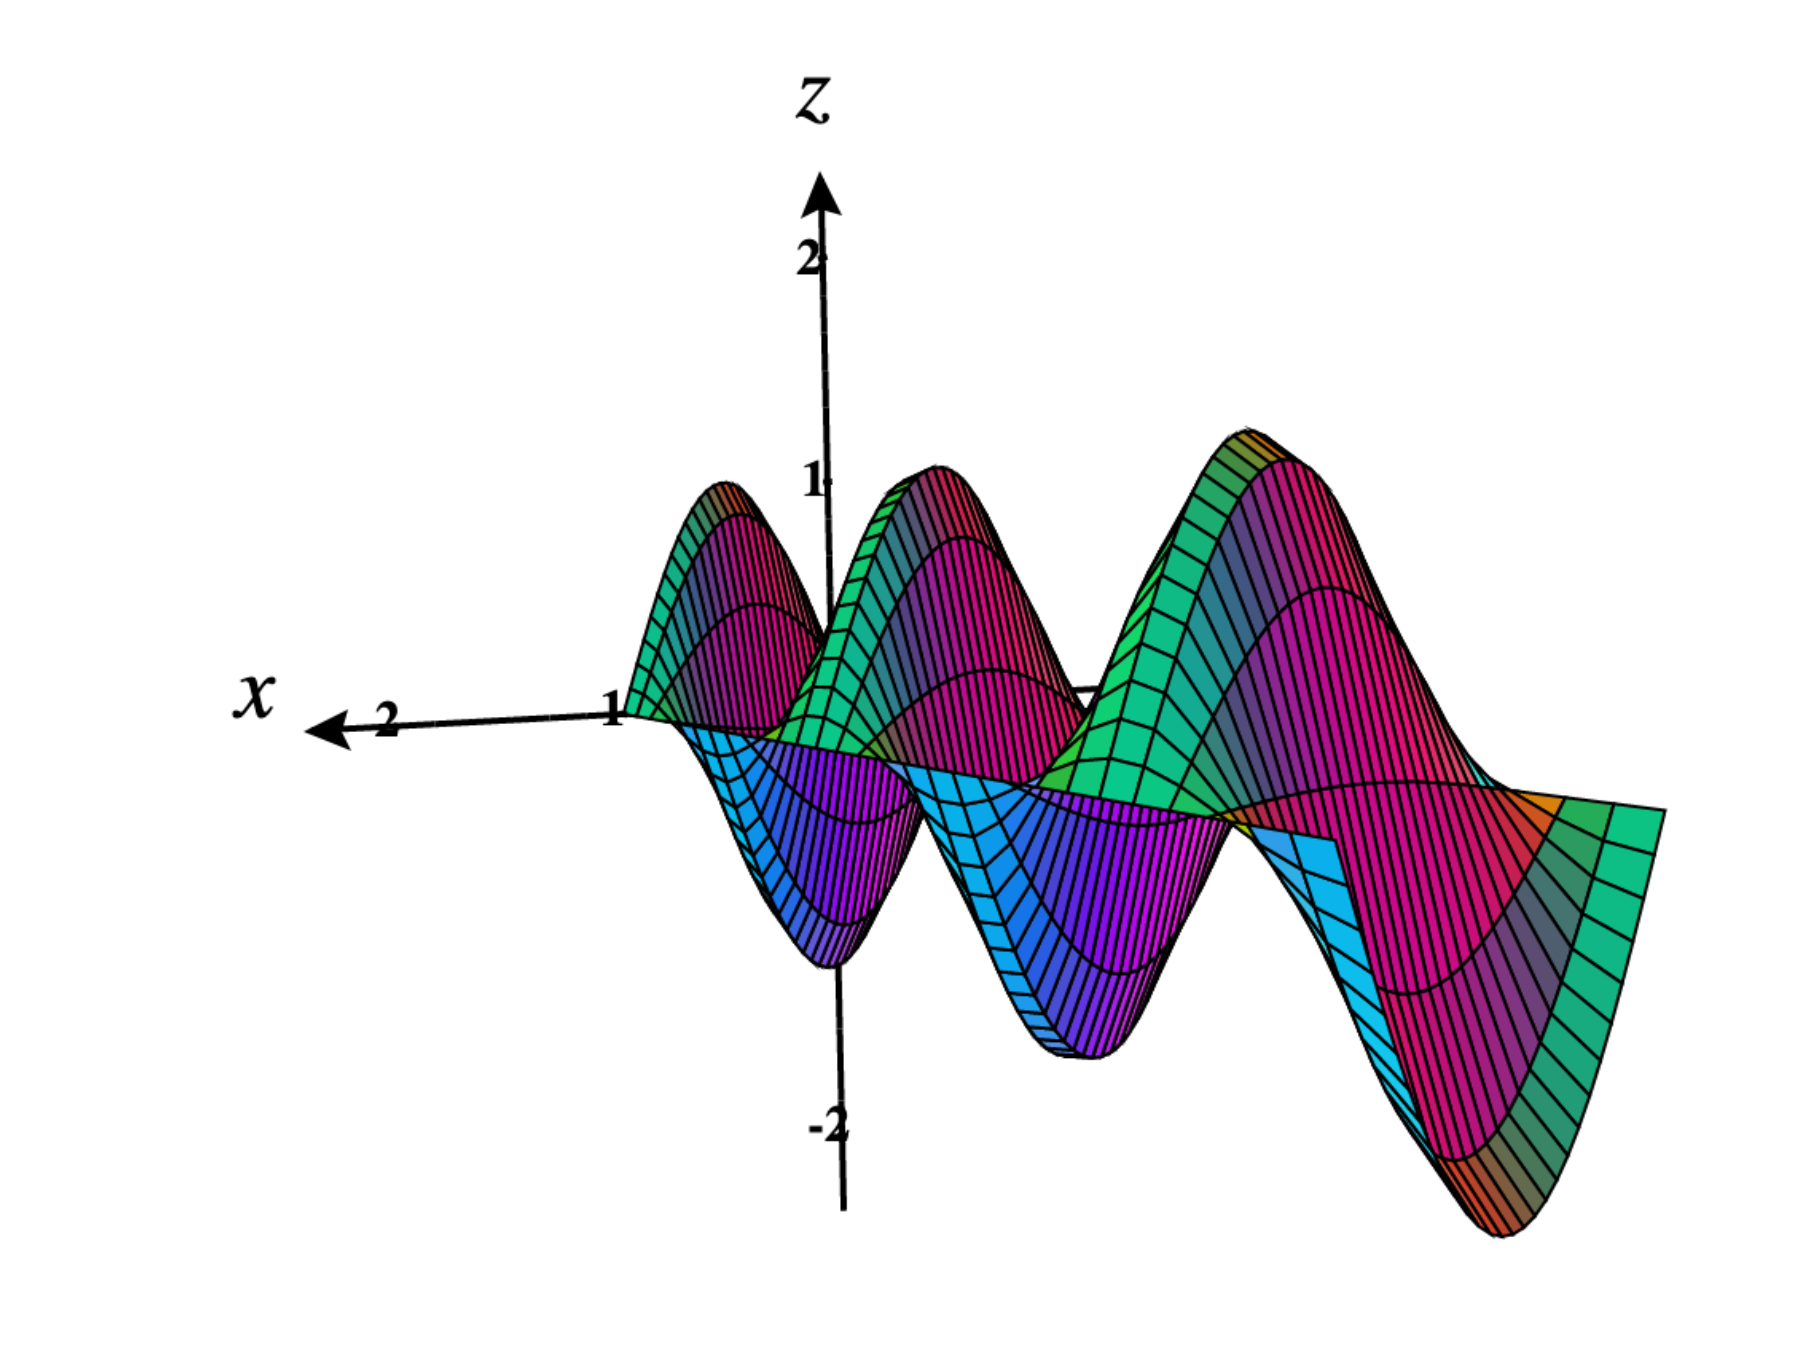
\includegraphics[width=.5\textwidth]{Figures/wave_solution.png}
        % \end{figure}
        \end{ex}

% \end{document}

%
%\chapter{Separation of Variables}
%\input{Chapters_Part_7/separation_of_variables.tex}
%
%\chapter{Fourier Transforms and Harmonics}
%\input{Chapters_Part_7/fourier_transforms_harmonics.tex}


%\chapter{Remarks for Math 271}
%So far, we have covered a broad spectrum of topics. Many of these topics are not typical for a calculus II student, while some were.  Instead of taking the typical path through calculus II, then calculus III, we are venturing in a way that allows us to tell a story and build a firm foundation in mathematics specifically used throughout chemistry (and especially physical chemistry).  Typically, students in the calculus sequence learn differentiation and integration in a first course.  In a second course, students learn about sequences, series, power series, and Taylor series.  The third course entails learning calculus in higher dimensions. Specifically, one concentrates on calculus in 3-dimensional space since this is (arguably) the most physically meaningful to us.  Following the calculus sequence comes a course in differential equations where students are granted a handbook of techniques for solving different types of equations.

We approached this in a completely different way.  We began by studying complex numbers as this field of numbers allows us to factor polynomials.  The complex numbers also formed a vector space, and we briefly investigated this structure.  However, the main goal was to use these complex numbers in order to be able to solve many different first and second order differential equations.  These differential equations arose by studying systems that change over time. For example, we saw the harmonic oscillator equation arise from a spring/mass system. We also saw that chemical reactions were nicely described by differential equations. Those equations were describing systems that evolved over time and were given with initial function values at time zero. Another way differential equations arose was via boundary value problems. In particular, we studied the free particle in a one-dimensional box and came across many new concepts that resurface later.

Quickly, one sees that the techniques we used to solve differential equations were not all powerful. Thus, we sought out a new technique to solve more equations.  Eventually, we arrived at power series which provided us with newfound abilities to compute.  For example, one needs a tool such as a power series to compute values to the function $\sin(x)$!  Power series then proved as indispensable tools for solving more differential equations than we were previously able to work with.  When we still had trouble with a specific equation, we could then use a Taylor series to find polynomial approximations of terms in a differential equation and from there we could solve this equation using power series.  This part of the class was closer to a typical calculus II course but came with the added bonus of solving differential equations as well.  Even in a first course on ordinary differential equations, one may not solve equations using a power series! 

Finally, the last portion of this class came as a preparation to deal with higher dimensional spaces.  Understanding vector spaces and how they transform is a necessary building block to studying calculus in higher dimensions.  However, linear algebra can be done in more generality than we have covered here.  In this generality, we can see how topics we have previously worked with fit in as well.  For example, we spoke of linear differential equations and one can show that the set of solutions to a linear differential equation forms a vector space! Either way, the lessons that linear algebra teaches us about geometry and using geometrical tools to solve problems is highly important.  This can lead one to considering abstracting algebra further and seeing if that can help solve problems as well.  

Next, we move onto the sequel of Math 271 which is Math 272 where we will spend time learning calculus in higher dimensions.  In order to model the physical world, this is completely necessary.   The topics covered in 271 will lead straight into the new mathematics awaiting us in 272.  Keep these previous chapters as a reference as they are now prerequisite material!


 
\newenvironment{changemargin}[1]{%
\begin{list}{}{%
\setlength{\topsep}{#1}
\setlength{\listparindent}{\parindent}%
\setlength{\itemindent}{\parindent}%
\setlength{\parsep}{\parskip}%
}%
\item[]}{\end{list}}

\begin{changemargin}{0cm}
\printindex 
\end{changemargin}

 
\end{document}